%! TEX TS-program = lualatex
\documentclass[12pt,a4paper,oneside]{article}

\usepackage[backend=biber, style=iso-numeric]{biblatex}
\addbibresource{src/biblio.bib}
% Definice vlastního formátu citace pro čísla v hranatých závorkách
\DeclareFieldFormat{labelnumberwidth}{\mkbibbrackets{#1}}
\DeclareFieldFormat{shorthandwidth}{\mkbibbrackets{#1}}

\input{/home/tom/Tools/TeX_tools/templates/protocol/src/_preamble.tex}
\geometry{left=30mm,right=30mm,top=35mm,bottom=40mm} % okraje pro elektronickou verzi PDF 
% \geometry{left=30mm,right=30mm,top=35mm,bottom=40mm} % okraje pro tištěnou a vázanou verzi PDF 

% \usepackage[left=30mm,right=30mm,top=35mm,bottom=40mm]{geometry} % nastavuje okraje stranky
\usepackage{float}
\usepackage{multirow}
\usepackage{longtable}
\usepackage{pdfpages}
\usetikzlibrary{decorations.pathreplacing, calligraphy}
\usepackage{hyperref}

\newcommand{\todo}[1]{
	{\color{red}\textsuperscript{\tiny \texttt{TODO}}\footnotemark\footnotetext{\scriptsize{}#1}}
}
\renewcommand\lstlistingname{Výpis}

\begin{document}
\def\projekt{TAČR SIGMA\_DC3 \enquote{\emph{Telemedicínské samovyšetření řeči a paměti pro rychlou detekci kognitivních poruch metodami strojového učení}}}

%! Author = tom
%! Date = 05.05.22

% Preamble
%\documentclass[12pt,a4paper,oneside]{article}
%\author{Tomáš Lebeda}

%\input{/home/tom/Tools/TeX_tools/src/myPreamble.tex}
%\mySetup
%\date{}
% Packages
%\renewcommand{\baselinestretch}{1.4} % nastavení řádkování 1,5
\thispagestyle{empty}
% Document
%\begin{document}
\begin{Large}
	\vspace*{-1cm}
	\begin{center}
		\textbf{Západočeská univerzita v~Plzni\\Fakulta aplikovaných věd\\Katedra kybernetiky}\\
		\vspace*{7cm}
		\begin{LARGE}
			\textbf{DIPLOMOVÁ PRÁCE}\\
		\end{LARGE}
	\end{center}
\end{Large}
\vspace*{8cm}
\begin{large}
	\hspace*{-5mm}\textbf{PLZEŇ, 2024}\hfill \textbf{Bc. Tomáš LEBEDA}\hspace*{-5mm}
\end{large}
%\end{document}

\clearpage
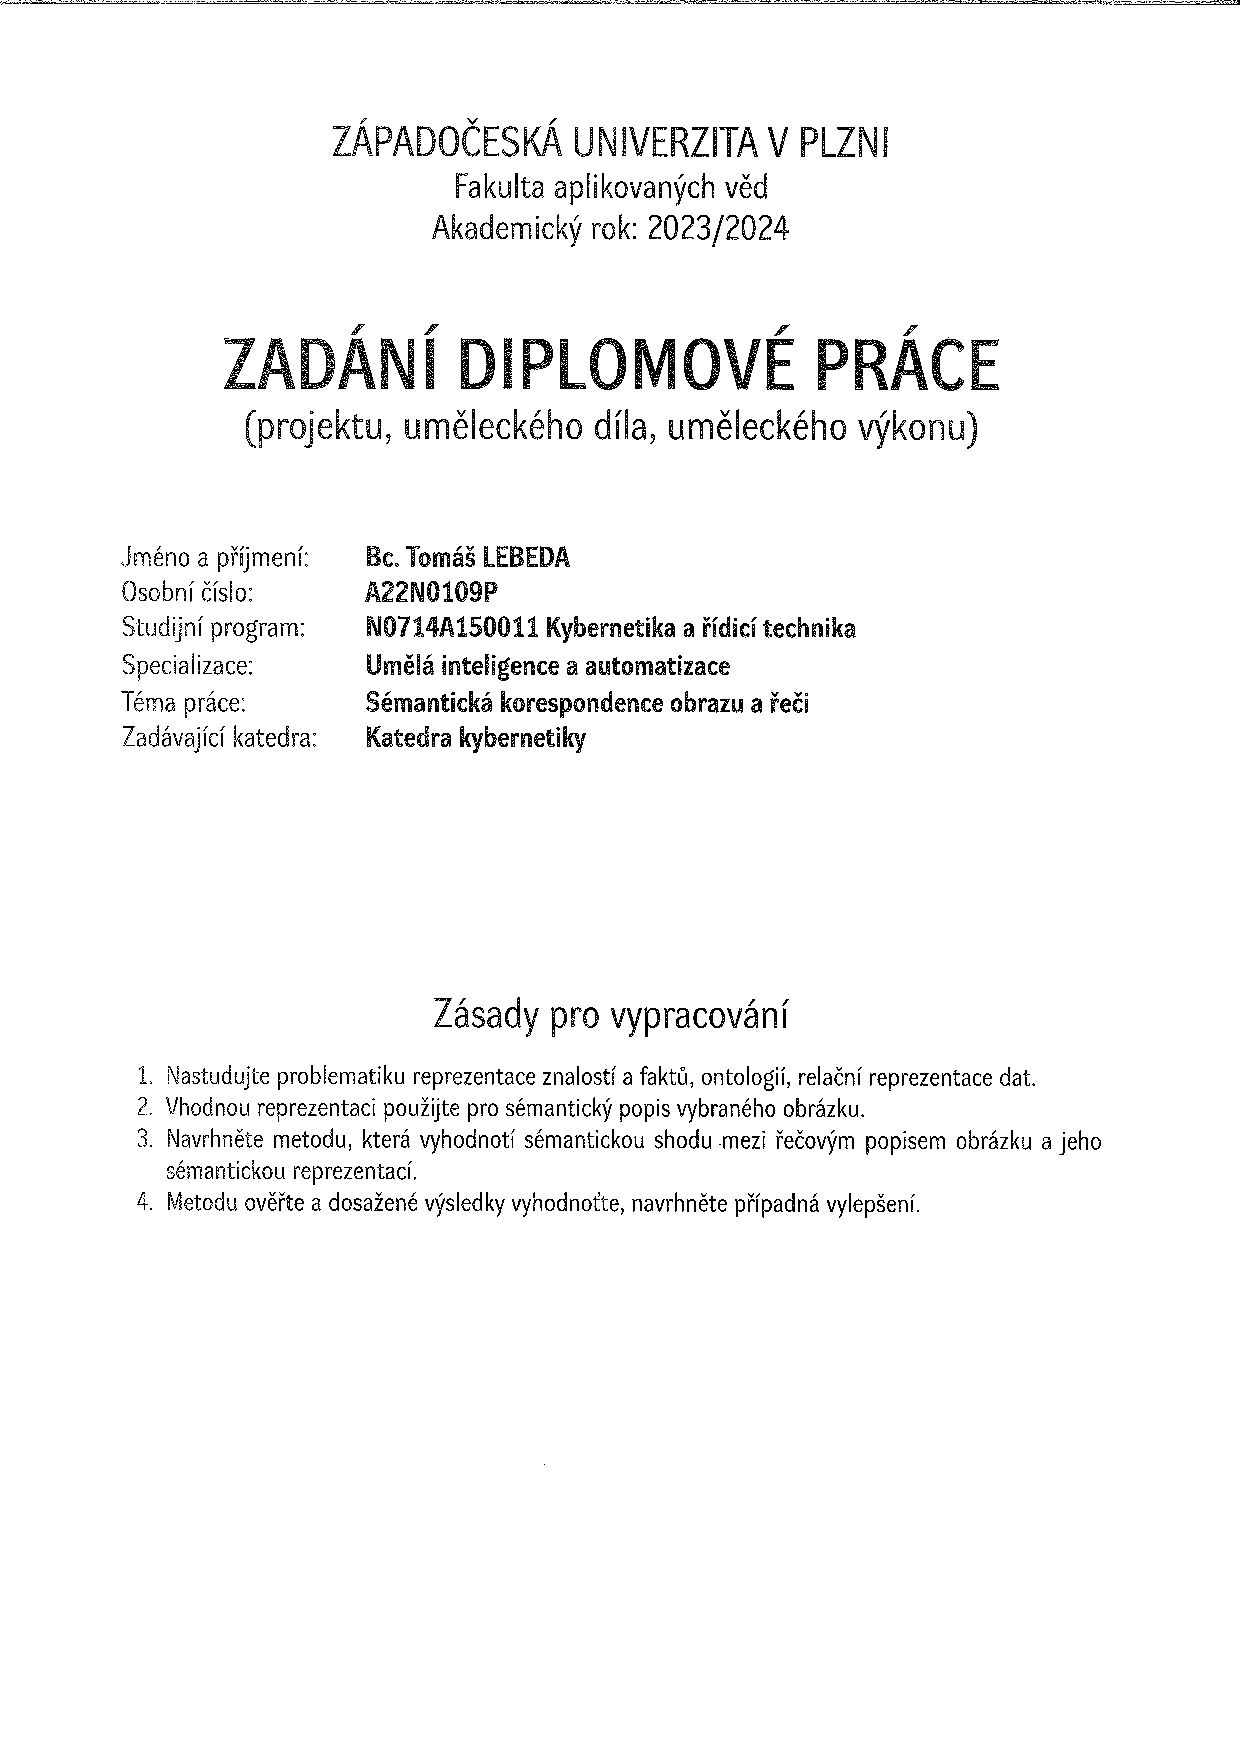
\includepdf[page=1,trim=0mm 0mm 0mm 0.0mm, angle=0.2]{src/imgs/zadani1.pdf}
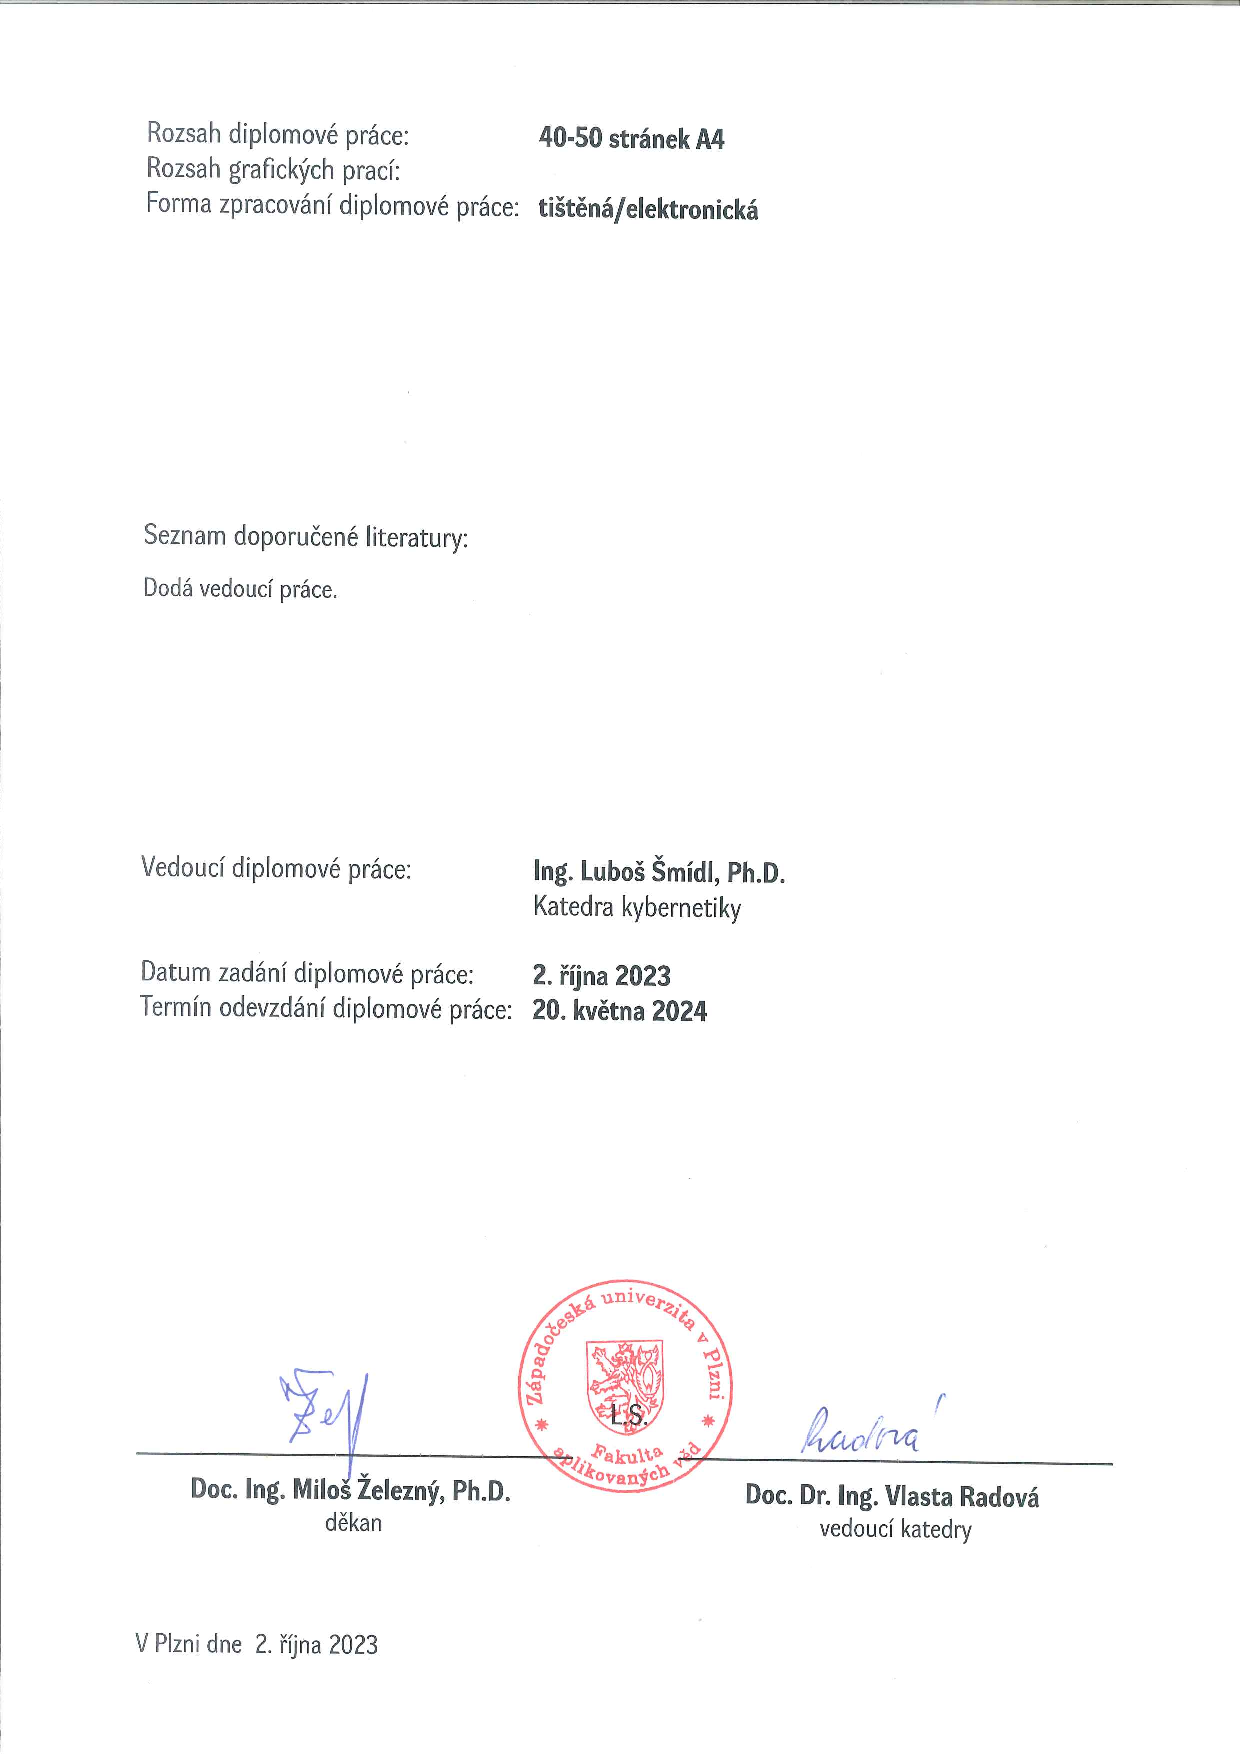
\includepdf[page=1,trim=0mm 0mm 0mm 0.0mm, angle=0.6]{src/imgs/zadani2.pdf}
\tableofcontents

\clearpage
\section{Úvod}
% NOTE: obecně oblast - co to je, k čemu se to používá
V současném výzkumu aplikované lingvistiky a počítačového zpracování přirozeného
jazyka zaujímá oblast zpracování textu, sémantická analýza a reprezentace znalostí význačnou pozici.
Tyto problematiky jsou nedílnou součástí mnoha běžně používaných systémů,
mezi které patří dnes již běžně dostupní hlasoví asistenti, automatické překlady a titulkování,
či systémy pro extrakci informací v různých průmyslových nasazeních.
% Ve všech těchto nasazeních jsou nějakou formou řešené také problémy sémantiky a reprezentace znalostí, 
% jakožto nedílné součásti těchto řešení.
% Kromě průmyslových a komerčních aplikacích se však zpracování přirozeného textu a sémantická analýza
% uplatňuje i v řadě dalších, více specializovaných oblastech, jako je například medicína,
% kde jsou tyto koncepty používané například pro automatické zpracování a extrakci informací.

% NOTE: co bude v této práci + motivace
Cílem této práce je navrhnout a implementovat systém pro určení míry korespondence obrázku a jeho popisu v přirozené řeči, a to na sémantické úrovni.
Motivací pro takovýto systém je možnost jeho využití pro vytvoření aplikace usnadňující vyšetření pro detekci kognitivních
poruch s využitím metod strojového učení.
Základní myšlenkou je využití předpokladu, že snížené kognitivní funkce se projeví mimo jiné
i na schopnosti člověka detailně popsat komplexní scénu zobrazenou na předloženém obrázku.

Hlavní koncept prezentovaný v této práci spočívá v extrahování sémantické informace obsažené v přirozeném popisu,
srovnání se vzorovým popisem a ohodnocení míry korespondence v podobě vektoru hodnot, který je možné
následně použít jako vstup pro další zpracování, například jako vektor příznaků pro klasifikaci.

% NOTE: Na co byl kladen důraz
Během návrhu celkového konceptu systému, jeho jednotlivých částí a i následné implementace, byl kladen důraz na to,
aby byly jednotlivé procesy \enquote{průhledné}, bylo možné detailně sledovat všechny kroky
a v případě potřeby dělat detailní změny či vylepšení, pro zdokonalení výsledků v konkrétním nasazení.
S tímto faktorem souvisí i volitelná granularita vstupních dat i výstupního hodnocení, což opět přispívá k možnosti precizně
nastavit každou část pro co nejlepší výsledky v reálném nasazení.

Dále bylo dbáno na modularitu systému, aby bylo možné v případě potřeby jednotlivé části nahradit za případné alternativy, nebo doplnit dodatečnými rozšířeními.
Je vhodné poznamenat, že ačkoli bylo primární motivací již zmíněná podpora diagnostiky kognitivních poruch,
byl systém navrhován obecně tak, aby jej bylo možné použít i pro případná další nasazení benefitující ze zde navržených metod.

% NOTE: co je v práci popsáno
V práci bude popsán návrh jednotlivých částí i celkové architektury, včetně zdůvodnění učiněných rozhodnutí.
Následně bude popsána samotná realizace, společně s problémy a jejich řešením, které se v průběhu vypracování vyskytly.


\section{Teorie}
\subsection{Sémantika}

\subsection{Reprezentace znalostí}
Pro řešení prakticky každého reálného problému je potřeba mít k dispozici nějaké znalosti minimálně z oblasti, ve které se problém nachází.
Při řešení problémů pomocí automatický počítačových metod a metod umělé inteligence je pak nutné ještě navíc
mít nějaký způsob, jak tyto znalosti zapsat a uchovat, jak s nimi manipulovat a provádět na nich operace a algoritmy.

Znalost je možné chápat jako nějakou informaci, která popisuje určitý fakt, nebo \enquote{pravdu o světě}.
Jejich vyjádření v nějakém konkrétní podobě, neboli \emph{formalismu}, je potom označováno jako \emph{reprezentace znalostí}.
Tato formální vyjádření by měla umožňovat provádět se znalostmi potřebné operace k vyřešení daného problému.~\cite{prepreze_znal}

Nové znalosti je možné získat v základu dvěma způsoby.
Prvním z nich je pozorování objektů a jevů, což je označováno jako přímé získávání znalostí.
Druhou metodou, která označována jako nepřímá, je odvození nových znalostí z těch, které jsou již známé.~\cite{prepreze_znal}

\subsubsection{Dělení reprezentace znalostí}
Podle učebního textu~\cite{prepreze_znal} je možné metody reprezentace znalostí rozdělit do několika kategorií.
Schématické znázornění tohoto dělení je na Obrázku~\ref{fig:schema_repreznalosti}.
\begin{figure}[ht!]
	\centering
	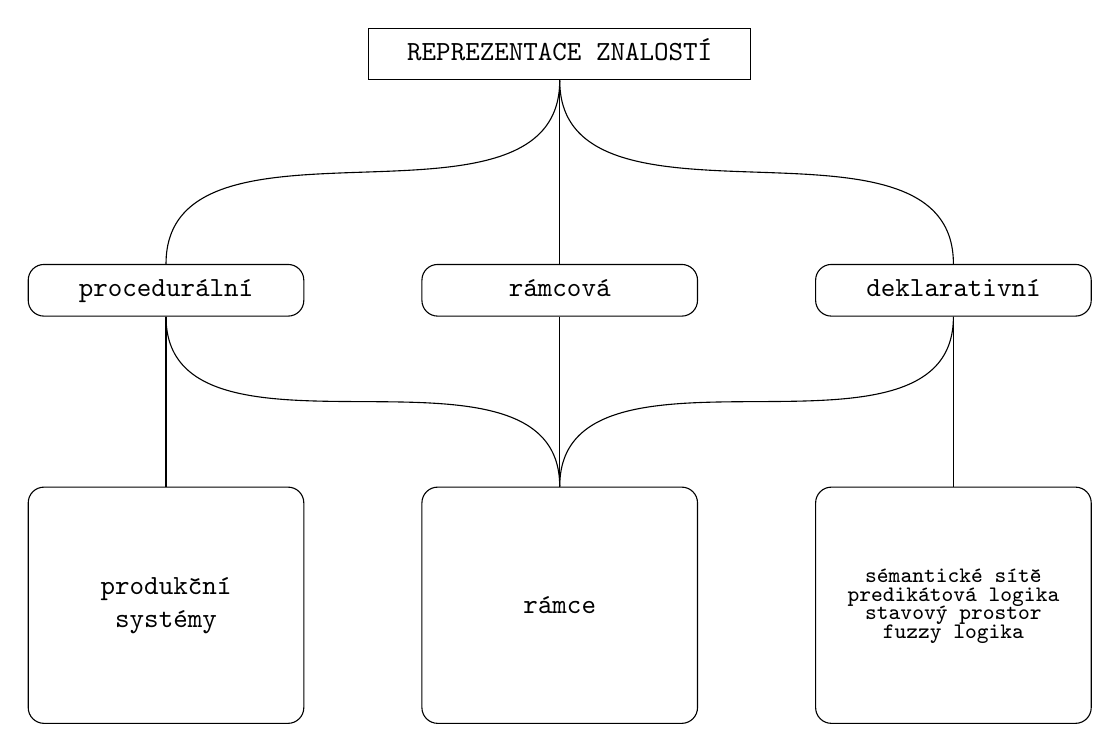
\begin{tikzpicture}
		\node[draw] (main) at (0, 0) {\strut\texttt{\phantom{ll}REPREZENTACE ZNALOSTÍ\phantom{ll}}};
		\node[draw,minimum width=3.5cm, rounded corners=2mm] (procedur) at (-5, -3) {\strut \texttt{procedurální}};
		\node[draw,minimum width=3.5cm, rounded corners=2mm] (dekl) at (5, -3) {\strut \texttt{deklarativní}};
		\node[draw,minimum width=3.5cm, rounded corners=2mm] (rámc) at (0, -3) {\strut \texttt{rámcová}};
		\node[draw,minimum width=3.5cm, minimum height=3cm, rounded corners=2mm] (prodsys) at (-5, -7) {\parbox{3cm}{\centering\texttt{produkční\\systémy}}};
		\node[draw,minimum width=3.5cm, minimum height=3cm, rounded corners=2mm] (mid) at (5, -7)
		{
			\footnotesize
			\begin{tabular}{c}
				\texttt{sémantické sítě}    \\[-1mm]
				\texttt{predikátová logika} \\[-1mm]
				\texttt{stavový prostor}    \\[-1mm]
				\texttt{fuzzy logika}
			\end{tabular}};
		\node[draw,minimum width=3.5cm, minimum height=3cm, rounded corners=2mm] (ramce) at (0, -7) {\texttt{rámce}};
		\draw[-] (main.south) to[out=-90, in=90] (procedur.north);
		\draw[-] (main.south) to[out=-90, in=90] (dekl.north);
		\draw[-] (main.south) to[out=-90, in=90] (rámc.north);
		\draw[-] (procedur.south) to[out=-90, in=90] (prodsys.north);
		\draw[-] (procedur.south) to[out=-90, in=90] (ramce.north);
		\draw[-] (rámc.south) to[out=-90, in=90] (ramce.north);
		\draw[-] (dekl.south) to[out=-90, in=90] (mid.north);
		\draw[-] (dekl.south) to[out=-90, in=90] (ramce.north);
	\end{tikzpicture}
	\caption{Schéma dělení metod reprezentace znalostí~\cite{prepreze_znal}}\label{fig:schema_repreznalosti}
\end{figure}

Deklarativní přístup je založený na vyjádření různých znalostí ve formě \emph{poznatků}, množinou konkrétních a navzájem nezávislých faktů.
S těmito fakty je pak možné manipulovat pomocí takzvaných \emph{procedur}, někdy označovaných jako tvrzení.
Mezi deklarativní metody se také řadí různé přístupy založené na matematice a logice, na algebře, relačních strukturách.
Mezi deklarativní metody se řadí \emph{sémantické sítě}, které znalosti reprezentují jako entity či objekty
relací, které mezi těmito objekty popisují jejich vztahy.
Dalším deklarativním typem reprezentace znalostí jsou \emph{stavové prostory},
které popisují řešený problém jako množinu možných stavů, ve kterých se daný problém může nacházet.
Mezi další formy reprezentace znalostí deklarativní povahy se řadí různé druhy logiky,
jako jsou \emph{predikátová logika} a \emph{fuzzy logika}.~\cite{prepreze_znal}

Procedurální metody reprezentace znalostí zahrnují produkční systémy.
To jsou systémy navržené tak, že pomocí předem dané množiny pravidel, které se označují jako produkční pravidla,
se snaží dosáhnout nějakého stanoveného cíle a vyřešení určitého problému.~\cite{prepreze_znal}

Poslední skupina, označená jako rámcová metoda reprezentace znalostí, představuje kombinaci obou předchozích přístupů.
Rámce jsou struktury, které popisují různé objekty podle předem dané formy a v průběhu řešení
problému se doplňují konkrétní hodnoty k daným vlastnostem.~\cite{prepreze_znal}

Schématická ukázka sémantické sítě využívající rámce je na Obrázku~\ref{fig:frames_net}
\begin{figure}[ht!]
	\centering
	\begin{tikzpicture}
		\node[inner sep=0pt] (n) at (0, 0) {
			\begin{tabular}{|l|l|}
				\hline
				\emph{Slot}           & \emph{Value}                   \\
				\hline
				\texttt{INSTANCE-OF}: & \texttt{(DOG, PET)}            \\
				Name:                 & \enquote{Fido}                 \\
				Color:                & \texttt{(BROWN)}               \\
				Father:               & \texttt{(BOWSER)}              \\
				Mother:               & \texttt{(WEENIE)}              \\
				Owner:                & \texttt{(MR.-SMITH)}           \\
				Cost:                 & \ \$12.95                      \\
				Has-as-ears:          & \texttt{(LEFT-EAR, RIGHT-EAR)} \\
				Number-of-ears:       & \texttt{(2)}                   \\
				\hline
			\end{tabular}
		};

		\node[draw=none] (n1) at (8, 0) {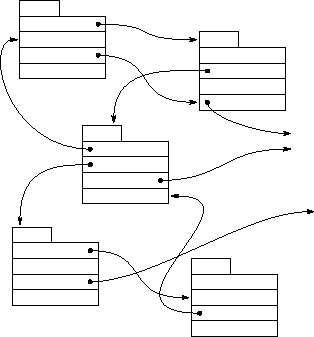
\includegraphics{./src/imgs/frames.pdf}};

		\node[draw, anchor=south west] at ($(n.north west) + (0, -0.5pt)$) {\texttt{(FIDO)}};
	\end{tikzpicture}
	\caption{Ukázka rámce pro individuálního psa (vlevo) a schématické znázornění propojení více rámců (vpravo), převzato z~\cite{semantic-nets-LEHMANN19921}}\label{fig:frames_net}
\end{figure}

\newpage
\subsubsection{Sémantické sítě}
Sémantické sítě reprezentují znalosti pomocí grafových struktur složených z uzlů a hran.
Uzly představují koncepty či objekty a hrany reprezentují relace mezi těmito jednotkami.
Ukázka jednoduché sémantické sítě je na Obrázku~\ref{fig:semantic_net_example}.

\begin{figure}[H]
	\centering
	\begin{tikzpicture}
		\node[draw, ellipse, minimum width=1.5cm, minimum height=1cm] (dog) at (0,0) {\texttt{pes}};
		\node[draw, ellipse, minimum width=2cm, minimum height=1cm] (sq) at (5,0) {\texttt{kočka}};
		\node[draw, ellipse, minimum width=2cm, minimum height=1cm] (tree) at (2,3) {\texttt{strom}};
		\node[draw, ellipse, minimum width=2cm, minimum height=1cm] (mush) at (5.5,3) {\texttt{kámen}};
		\node[draw, ellipse, minimum width=2cm, minimum height=1cm] (animal) at ($0.5*(dog) + 0.5*(sq) + (0, -2)$) {\texttt{zvíře}};
		\draw[-Stealth, bend left=25] (dog) to node[midway, above] {\footnotesize \texttt{běží za}} (sq);
		\draw[-Stealth] (dog) to node[midway, above] {\footnotesize \texttt{větší než}} (sq);
		\draw[-Stealth, bend left=25] (sq) to node[midway, above] {\footnotesize \texttt{utíká před}} (dog);
		\draw[-Stealth] (sq) -- node[midway, above, sloped] {\footnotesize \texttt{šplhá na}} (tree);
		\draw[-Stealth] (mush) -- node[midway, above, sloped] {\footnotesize \texttt{je pod}} (tree);
		\draw[-Stealth, bend left=30] (mush) -- node[midway, above, sloped] {\footnotesize \texttt{větší než}} (sq);
		\draw[-Stealth] (dog) to node[midway, above, sloped] {\footnotesize \texttt{je pod}} (tree);
		\draw[-Stealth, bend right=30] (dog) to node[midway, above, sloped] {\footnotesize \texttt{je}} (animal);
		\draw[-Stealth, bend left=30] (sq) to node[midway, above, sloped] {\footnotesize \texttt{je}} (animal);
	\end{tikzpicture}
	\caption{Ukázka jednoduché sémantické sítě}\label{fig:semantic_net_example}
\end{figure}

Sémantické sítě umožňují použít různé metody z teorie grafů, logiky a matematiky pro práce s uloženými znalostmi,
jejich analýzu a případně i odpovídání otázek či indukci nových znalostí.
Sémantické sítě se používají v oblastech umělé inteligence pro porozumění jazyku, deduktivní databáze, vyhledávání dokumentů
v databázi, expertní systémy a další.~\cite{semantic-nets-LEHMANN19921}

Sémantické sítě je možné realizovat také s využitím rámců (angl.~frames) pro jednotlivé uzly.
Rámec je chápán jako abstraktní popis nějakého objektu, která má pojmenované \emph{sloty}, které popisují nějaké explicitní vlastnosti.
Tyto rámce mohou být navzájem propojené a odkazovat se na sebe navzájem, čímž tvoří strukturu orientovaného grafu.
Některé implementace také poskytují možnost dynamického zjišťování hodnot pro jednotlivé sloty pomocí procedurálních metod,
což umožňuje zachytit komplexní chování a inferenci.~\cite{semantic-nets-LEHMANN19921}

Podle~\cite{semantic-nets-LEHMANN19921} je možné rozdělit vazby (hrany) v sémantických sítích do několika skupin.
V relačních grafech, kde hrany popisují relace mezi objekty, tak se označují jako \emph{deskriptivní} nebo \emph{asertivní}.
Oproti \emph{strukturálním}, \emph{definičním} nebo \emph{inferenčním} vazbám, které slouží k zachycení hierarchické struktury objektů,
popisují vyšší abstrakce, kategorie a dědičnost.~\cite{semantic-nets-LEHMANN19921}

Aby bylo možné pomocí sémantických sítí zachytit i principy logiky, jako jsou:
\begin{itemize}
	\item negace (např.~\enquote{kámen NENÍ zvíře}),
	\item disjunkce (např.~\enquote{osoba narozená v Británii NEBO potomek Brita}),
	\item existenční kvantifikátory (např.~\enquote{VŠECHNY cesty vedou do Říma}),
\end{itemize}
a další komplexnější vztahy, je možné sémantické sítě rozšířit o další typy vazeb (např.~IS-NOT-A) i celé strukturální koncepty,
jako je rozdělení sítě do \emph{prostorů}, které se mohou překrývat jako Vennovy diagramy, což umožňuje vyjádřit složitější logické operace.
Dalším typem rozšíření, který se vyskytuje v \emph{konceptuálních grafech}, je použití \emph{vnořených kontextů},
jejichž principem je využití metod logiky pro vyjádření složitějších operací skrze zapouzdření (angl.~encapsulation) primitivních operací.
~\cite{semantic-nets-LEHMANN19921}

\subsubsection{Ontologie}
Samotná forma reprezentace znalostí a způsob práce s nimi je pouze částí problematiky sémantických sítí,
druhou otázkou, kterou je potřeba řešit, je samotný obsah, neboli \enquote{co reprezentovat}.
Tímto problémem se zabývá \emph{ontologie}, která zahrnuje formální označení, strukturu a definice jednotlivých kategorií,
vlastností, relací a samotných dat, které je potřeba reprezentovat.
Existuje řada různých přístupů a realizací, příkladem může být projekt \emph{Cyc}~\cite{cyc}, jehož cílem je poskytnout ontologii pro reálný svět.
Jiným příkladem může být J. L. Jolleyův \emph{Holotheme}~\cite{jolley1971holotheme}, který se také snaží klasifikovat cokoli,
ovšem v rámci jednoho schématu založeného na strukturální komplexitě.
Dalším příkladem je \emph{Wordtree}~\cite{burger1984wordtree}, který představuje pokus o definici významů slov pomocí kombinování primitivních konceptů a významů.~\cite{semantic-nets-LEHMANN19921}

% \clearpage
\section{Korespondence obrazu a jeho slovního popisu}
Korespondence mezi obrazem a jeho popisem je problematika řešená v řadě reálných praktických aplikací.
Tato kapitola popisuje základní principy práce s obrazem a spojitost s jeho popisem, a některé vybrané příbuzné problémy.
Na závěr jsou v této kapitole zmíněné rozdíly v přístupu, který byl zvolen pro tuto práci.

\subsection{Práce s obrazovými daty}
Popis obrázku je v kontextu výpočetní technologie a umělé inteligence rozšířené téma, které nachází uplatnění v mnoha praktických aplikacích.
Jedná se o jednu z mnoha problematik, které se obecně v úlohách počítačového zpracování obrazových dat řeší.

Úlohy, které se týkající zpracování obrazu, lze podle učebního textu~\cite{conv-gruber} rozdělit do čtyř základních typů:
\begin{enumerate}
	\item \textbf{Klasifikace}\\
	      Jedná se o úlohu přiřazování obrázku k nějaké třídě.
	      Množina tříd, do kterých jsou obrázky přiřazované, jsou často známé předem a může jich být různá množství,
	      od několika jednotek pro úzce specializované úlohy, například v medicíně, nebo pro obecnější úlohy u tisíce.

	      V úlohách klasifikace není brán ohled na prostorové informace, celý obrázek je chápán jako jeden celek,
	      jemuž je přiřazena příslušnost do vybrané třídy.
	      Typickým příkladem může být rozdělení obrázku do kategorií \emph{kočka} nebo \emph{pes} podle toho,
	      jaké zvíře je na obrázku znázorněno.
	\item \textbf{Sémantická segmentace}\\
	      Sémantická segmentace obrázků spočívá v přiřazení nějaké ze tříd každému pixelu.
	      Tím dojde k rozdělení obrázku do disjunktních oblastí, které jsou (sémanticky) označené danou třídou.

	      V úlohách tohoto typu se již patrně zohledňuje prostorová informace jednotlivých částí,
	      avšak jednotlivé instance různých objektů pod společnou třídou rozlišené nejsou.
	      Příkladem typické segmentace může být určení toho, které pixely odpovídají obloze, které zemi, a které třeba člověku.

	      \newpage
	\item \textbf{Detekce objektů}\\
	      Principem detekce objektů je v obraze určit, zda se v něm nachází jeden nebo více hledaných objektů daného typu.
	      Vstupem bývá obrázek a požadavek na detekci nějakého typu objektu a výstupem může být obrázek s označením
	      objektů pomocí ohraničujících rámců (angl.~bounding-box) s přiřazeným označením třídy.

	      Tento typ úlohy může být vhodný například pro sledování (tracking) lidí či zvířat, pro následnou klasifikaci nebo jinou analýzu.

	\item \textbf{Segmentace instancí}\\
	      Tento typ úlohy představuje kombinaci předchozích typů úloh.
	      Princip spočívá v tom, že v obrázku jsou označené pixely odpovídající nějakému hledanému objektu stejně jako při
	      sémantické segmentaci, ovšem s tím rozdílem, že není nutné takto označit každý pixel v obrázku a naopak je
	      dbáno na rozlišení jednotlivých instancí daných objektů.

	      Výsledkem je tedy informace o tom, které pixely odpovídají jakému konkrétnímu objektu.
	      Například na obrázku, kde by bylo zobrazeno více psů a koček, by bylo cílem označit kde přesně se nachází
	      který pes a která kočka.
\end{enumerate}

Všechny výše zmíněné typy úloh, respektive jejich výstupy, lze považovat za popis obrázku v tom smyslu,
že výstupem je jistá forma informace o tom, co daný obraz zachycuje.
Nejedná se však přímo o hluboké či komplexní sémantické znalosti, spíše o \enquote{hrubé} zařazení do nějaké třídy nebo forma výpisu zobrazených objektů.

V současnosti jsou obrazová data zpracovávána převážně pomocí velkých neuronových sítí.
Díky pokrokům ve výpočetní síle a dostupnosti datových sad jsou tyto modely stále sofistikovanější a schopné řešit složitější úkoly.
Součástí tohoto pokroku je také schopnost modelů analyzovat obrazová data a v kombinaci se zpracováním přirozené řeči i
odpovídat na otázky týkající se komplexnější sémantiky.
{\footnotesize\color{red} [přidat zdroj, třeba na ten nový GPT-4o, kde je ukázka? Tady nemám přímo nic faktického, tak by to mohlo stačit? Tenhle odstavec je hlavně pro nějaké \enquote{napojení} popisu obrázků na sémantiku]}

\newpage
\subsection{Sémantický popis obrazu}
Jednou z oblastí, kde je využívána ontologie a sémantický popis obrázku, jsou systémy pro vyhledávání obrázků (angl.~image retrieval).

Například Sarwar et al.~\cite{SARWAR2013285} prezentuje metodu zabývající se zdokonalením přesnosti vyhledávání obrázků,
na základě vstupního dotazu v přirozeném jazyce.
Navrhuje metodu, která má tohoto cíle dosáhnout za využití doménové ontologie, lokální sémantické informace v podobě
obrazových deskriptorů a jejich kvalitativní prostorové relace.
% V rámci vyhledávání využívá pro práci s dotazy také dříve zmíněný RDF standard jako náhradu za běžně užívané postupy založené na klíčových slovech.
Navržená architektura v první fázi předzpracuje poskytnuté obrázky tak, že je rozdělí na jednotlivé sektory, kterým jsou
přiřazené značky reprezentující obecné, předem určené, koncepty, jako jsou například \enquote{tráva}, \enquote{nebe} nebo \enquote{písek}.
% Takto anotované obrázky je pak možné rozdělit do předem definovaných kategorií.
Další část architektury, kterou Sarwar et al.~\cite{SARWAR2013285} prezentuje, slouží k transformování uživatelského vstupu (dotazu)
do několika předem definovaných forem využívajících RDF triplety.
Poslední fází zpracování je pak využití doménové ontologie pro určení sémantické podobnosti dotazu a dostupných anotovaných obrázků,
ze kterého plyne výběr výstupního obrázku odpovídající vstupnímu dotazu.

Další příbuznou problematikou je automatická tvorba sémantických popisků k obrázkům, kterou
ve své práci prezentuje Meiyu et al.~\cite{img_semantic_descr_annotation}.
Využívá k tomu SIFT~\cite{sift} deskriptorů, kvůli jejich dobrému poměru mezi výpočetní náročností, informačním objemem a spolehlivostí.
Následně je v práci~\cite{img_semantic_descr_annotation} prezentováno, že díky internetu a z něj plynoucímu množství koexistujících
obrázků a jejich textových popisů, byl sestaven model, který je schopen mapovat extrahované příznakové vektory (angl.~feature vector)
ze SIFT deskriptorů na textové anotace, ze kterých jsou získané sémantické popisy.
Výsledky, které Meiyu et al.~\cite{img_semantic_descr_annotation} prezentuje, pak zobrazují obrázek,
k němuž jsou automaticky doplněné anotace objektů a konceptů, které se na něm vyskytují.

Doposud popisované problémy a jejich řešení využívají převážně neuronových sítí a statistických metod,
jejichž základním předpokladem je dostatečný počet a kvalita trénovacích dat.

Vzhledem k motivaci této práce, kterou je hodnocení kvality popisu daného obrázku na sémantické úrovni pro
usnadnění detekce kognitivních poruch, byl zvolen expertní přístup se zaměřením na
kvalitativní analýzu výsledků, průhlednost celého procesu s možností detailních úprav a reprodukovatelnost.


% Zde navržený a implementovaný systém se zaměřuje na hodnocení kvality popisu obrázku v přirozené řeči, 
% kde vstupní 
% předpokládá pečlivě vytvořená a anotovaná data, která lze využít opakovaně 

% 1. Popisy obrázků jsou nejčastější formou nějaký klasifikace nebo detekce, založený na deskriptorech (sifty, surfy, ...) nebo přes velký neuronovky

% 2. Sémantika se u obrázků řeší spíš formou vytváření popisků (generování textu) nebo opačně - generovat obrázek z textu

% 3. Přímo sémantika obrázku a srovnat se sémantikou textu jsou maximálně nějaký přiřazovačky (vyhledávače obrázků)



\section{Návrh a architektura systému}\label{sec:navrh_architektura}
\subsection{Obecná architektura systému}
Obecná architektura celého systému vychází z jeho požadované funkčnosti,
kterou je porovnání obrázku s jeho popisem v přirozené řeči, a to na sémantické úrovni.
Z toho pak plyne, že celý systém se ve své podstatě skládá ze tří základních částí:
\begin{enumerate}
	\item referenční (vzorový) popis daného obrázku
	\item sub-systém pro zpracování přirozené řeči a tvorbu testovaného popisu
	\item porovnání referenčního a testovaného popisu
\end{enumerate}

Jednotlivé části spolu vzájemně fungují následujícím způsobem:
Uživateli je prezentován obrázek a jeho úkolem je popsat, co na obrázku vidí.
Získaný popis v přirozené řeči je převeden na text pomocí systému pro rozpoznání řeči (angl.~automatic speech recognition, ASR).
Z tohoto přepisu je extrahována sémantická informace, ze které je vytvořen testovaný popis.
Testovaný popis je porovnaný s referenčním (vzorovým) popisem daného obrázku.
Výsledek tohoto porovnání lze pak považovat za finální výstup, ale také je možné jej použít jako vstup pro další zpracování
(např.~vektor příznaků pro klasifikátor).
Schématické znázornění je na Obrázku~\ref{fig:architecture_scheme}.

\begin{figure}[H]
	\centering
	\begin{tikzpicture}[minimum width=2.5cm, minimum height=1cm]
		\node[anchor=south, inner sep=4pt, minimum height=0cm] (img) at (0,0) {\texttt{obrázek}};
		\node[draw] (user) at (-3,-1.5) {\texttt{UŽIVATEL}};
		\node[draw] (exp) at (3,-3.5) {\texttt{EXPERT}};
		\node[draw] (asr) at (-3,-3.5) {\texttt{ASR + SLU}};
		\node[draw] (comp) at (0,-6) {\texttt{KOMPARÁTOR}};
		\draw[-Stealth,rounded corners=2mm] (0,0) -- (0,-0.4) -| (exp.north);
		\draw[-Stealth,rounded corners=2mm] (0,0) -- (0,-0.4) -| (user.north);
		\draw[-Stealth] (user) -- node[minimum width=0cm,anchor=west,midway] {\texttt{řeč}} (asr);
		\draw[-Stealth,rounded corners=2mm] (asr) |- node[minimum width=0cm,right, near start] {\parbox{2cm}{\texttt{testovaný}\\[-3mm] \texttt{popis}}} (comp.west);
		\draw[-Stealth,rounded corners=2mm] (exp) |- node[minimum width=0cm,right, near start] {\parbox{2cm}{\texttt{referenční}\\[-3mm] \texttt{popis}}} (comp.east);
		\draw[-Stealth] (comp.south) -- node[midway, right, minimum width=0cm]{\texttt{hodnocení}} ++(0, -1);
	\end{tikzpicture}
	\caption{Schéma obecné architektury systému}\label{fig:architecture_scheme}
\end{figure}

Tato práce řeší problematiku srovnání obrázku s jeho popisem v přirozeném jazyce na sémantické úrovni expertním přístupem.
Od toho se poté odvíjí konkrétní algoritmy, formáty a postupy navržené a implementované v této práci,
které jsou podrobněji popsány v pozdějších kapitolách.
Je ale vhodné zmínit, že během návrhu bylo dbáno na to, aby bylo možné pro reálná nasazení některé implementace v případě potřeby zaměnit nebo upravit,
aby lépe vyhovovaly specifickým požadavkům pro dané použití.

Jak je možné ze schématu na Obrázku~\ref{fig:architecture_scheme} vidět, lidský expert je potřebný pro vytvoření referenčního popisu obrázku
(a také pro další vstupní data pro komparátor, popsáno později).
Všechna tato data, která jsou závislá na lidském expertovi, je ovšem možné vytvořit pouze jednou v rámci přípravy
a poté je lze již bez nutnosti přítomnosti experta opakovaně používat.

\subsection{Reprezentace znalostí}\label{subsec:reprezentace_znalosti}
Pro porovnání obrázku s jeho popisem v přirozené řeči bylo nutné zvolit či navrhnout takovou formu reprezentace znalostí,
která by umožnila zachytit sémantiku z obou zdrojů.
Jak již bylo výše zmíněno, zvolen byl expertní přístup, a to v tomto případě znamená, že referenční popis obrázku je vytvořen lidským expertem,
což klade další omezení na formát reprezentace znalostí.

Expertní přístup umožňuje velmi přesnou kontrolu nad obsahem a kvalitou vstupních dat, na rozdíl od automaticky získaných dat pomocí statistických metod.
To je výhodné hlavně z toho důvodu, že kvalita referenčního popisu a dalších vstupních dat přímo ovlivňuje kvalitu výstupu.
Další výhodou je průhlednost celého procesu, na rozdíl například od neuronových sítí, jejichž funkce je často označována jako black-box.
To je také spojeno s možností dělat v případě potřeby drobné změny a opravy chyb v referenčním popise.

Při návrhu bylo tedy potřeba brát v úvahu následující požadavky a najít nějaký formát, který by představoval vhodný kompromis mezi nimi.
\begin{itemize}
	\item \textbf{Čitelnost člověkem}:\\
	      Aby byl lidský expert schopen vytvořit, číst a případně upravit referenční popisy,
	      je nutné, aby byl schopen porozumět formě a zápisu uložených dat.
	      Toto omezení tedy upřednostňuje textové formáty a prakticky vyřazuje binární data.

	      Výjimku by mohl tvořit nějaký binární formát s přidruženým editorem,
	      kde by člověk mohl v grafickém prostředí prohlížet a manipulovat data, ale takový případ je nad rámec této práce.
	\item \textbf{Kompaktnost a struktura dat}:\\
	      Dalším důležitým aspektem je struktura a kompaktnost dat.
	      Pomocí počítače je poměrně snadné v krátkém čase zpracovat velké množství jednoduchých datových záznamů,
	      nicméně člověk se bude lépe orientovat v nějakém kompaktnějším popisu, který ačkoli může být složitější ve své struktuře,
	      tak bude pro člověka lépe názorný a uchopitelný.
	\item \textbf{Univerzálnost formátu}:\\
	      Podstatnou vlastností pro hledanou reprezentaci znalostí je její schopnost zachytit popis různých obrázků.
	      Navržený formát tedy musí být dostatečně univerzální, aby pomocí něj šlo popsat co nejširší spektrum informací,
	      od jednoduchých obrázků zobrazujících například jeden statický objekt, přes složitější obrázky zobrazující více objektů,
	      až po dynamické komplexní scény zobrazující mnoho objektů, činnosti a vazby mezi nimi.
	\item \textbf{Počítačová zpracovatelnost}:\\
	      V neposlední řadě je také potřeba dbát na to, aby navržený formát bylo možné co nejsnadněji zpracovat programově, na počítači.
	      Dynamické formáty s volnou strukturou bývají složitější na strojové zpracování, než fixní formáty s přesně definovanou podobou.
\end{itemize}

S ohledem na tyto body byla navržena reprezentace znalostí založená na sémantických sítích,
která definuje 4 základní \emph{aspekty popisu}: objekty, jejich hierarchii, statické atributy a dynamické vazby.
Detailnější popis těchto jednotlivých aspektů je v následujících částech,
konkrétní technická implementace je pak popsána v sekci~\ref{sec:implementace}.

\newpage
\subsubsection{Objekty ve scéně}\label{subsubsec:objekty_ve_scene}
\newcommand{\objekt}{{\color{red!70!black}\texttt{objekt}}}
Cokoli, co lze v obrázku ohraničit rámečkem (angl.~bounding-box)
a při separaci od zbytku scény neztratí nebo nezmění svůj význam,
lze považovat za \emph{objekt}.

Jako objekt v obrázku lze tedy označit zobrazené fyzické předměty, postavy, zvířata, ale také nehmotné pojmy jako \enquote{nebe},
místa, lokace či místnosti (např.~\enquote{kuchyň} nebo \enquote{louka}) a části jiných objektů (např.~\enquote{obličej}
jsou součást hlavy nebo celého člověka).

Tato definice objektu byla záměrně navržena velmi obecně, aby byl definovaný formát univerzální a šel použít i pro
popis velmi odlišných obrázků s různými účely.
Potenciální nevýhodou, která plyne z univerzálnosti formátu, může být v některých situacích problém nejednoznačnosti.

V jednom obrázku lze definovat různé množiny objektů, podle toho, jak moc detailní popis expert vytvoří.
Například pokud by byl na obrázku člověk, lze jej popsat jedním objektem jako \enquote{člověk} nebo \enquote{osoba},
ale také by šlo definovat ještě mnoho dalších objektů, například pro jednotlivé části těla nebo oblečení.

Kromě různých úrovní detailů lze také na problematiku nejednoznačnosti narazit v situaci, kdy je pro nějaký (dostatečně komplexní) obrázek
možné sestavit různé množiny objektů podle toho, pro jaké potřeby je zrovna obrázek a referenční popis používán.
Pro aplikaci, kde je podstatné zachycení živých objektů, může být množina objektů v referenčním popise tvořena lidmi či zvířaty.
Pro jiné použití pak ale může být podstatné zachytit prostředí a neživé předměty,
takže množina objektů by byla tvořena částmi prostředí (např.~stromy, křoví, voda, skály), budovami nebo obecnými předměty.

Příkladem obrázku s několika vyznačenými objekty je ilustrace na Obrázku~\ref{fig:object_image}.
\begin{figure}[H]
	\centering
	\def\dist{1pt}
	\begin{tikzpicture}[inner sep=0pt]
		\node[draw, inner sep=3pt] at (0, 0) {
\includegraphics[scale=0.35]{imgs/dog_squirrel_tree_mushroom.pdf}};
		\node[draw=red, minimum width=19mm, minimum height=14mm] (dog) at (-1.25, -1.85) {};
		\node[draw=red, minimum width=7mm, minimum height=8mm] (squirrel) at (0.14, -0.82) {};
		\node[draw=red, minimum width=10mm, minimum height=10mm] (mushroom) at (2.05, -1.82) {};
		\node[draw=red, minimum width=43mm, minimum height=55mm] (tree) at (0.64, 0.32) {};
		\node[red, anchor=south west] at ($(dog.north west) + (0, \dist)$) {\tiny pes};
		\node[red, anchor=south west] at ($(squirrel.north west) + (0, \dist)$) {\tiny veverka};
		\node[red, anchor=north west] at ($(tree.north west) + (\dist, -\dist)$) {\tiny strom};
		\node[red, anchor=south west] at ($(mushroom.north west) + (0, \dist)$) {\tiny houba};
	\end{tikzpicture}
	\caption{Ilustrace s vyznačenými objekty}\label{fig:object_image}
\end{figure}

\subsubsection{Hierarchie objektů}
Kromě množiny samotných objektů lze v obrázku také definovat jejich hierarchii.
To přirozeně plyne z výše zmíněné definice \emph{objektu}, která umožňuje specifikovat část existujícího objektu jako další samostatné objekty.

Příkladem takového popisu může být například situace, kdy je na obrázku strom.
Strom je možné rozdělit na korunu a kmen, korunu pak je možné dále dělit na větve.
Schématicky lze tento popis znázornit jako stromovou strukturu, viz Obrázek~\ref{fig:schema_hierarchie_objektu}.
\begin{figure}[H]
	\centering
	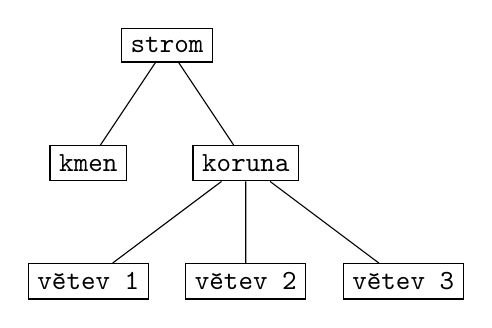
\begin{tikzpicture}[sibling distance=20mm]
		\node[draw, rectangle] {\texttt{strom}}
		child {node[draw, rectangle] {\texttt{kmen}}}
		child {node[draw, rectangle] {\texttt{koruna}}
				child {node[draw, rectangle] {\texttt{větev 1}}}
				child {node[draw, rectangle] {\texttt{větev 2}}}
				child {node[draw, rectangle] {\texttt{větev 3}}}
			}
		;
	\end{tikzpicture}
	\caption{Schématické znázornění hierarchie objektů}\label{fig:schema_hierarchie_objektu}
\end{figure}

Z pohledu daného objektu jsou \enquote{vyšší} (obecnější) objekty označované jako \emph{rodičovské objekty} (nebo jen \emph{rodiče}) a
\enquote{nižší} (konkrétnější) objekty pak jako \emph{potomci}.

Možnost definovat hierarchii objektů nabízí mimo jiné také způsob, jak vytvořit skupiny objektů, které k sobě nějakým způsobem patří.
Například strom může být součástí lesa, kráva může být součástí stáda nebo postava na hřišti může být součástí fotbalového týmu.
Tato příslušnost objektu nějaké skupině je dalším typem sémantické informace, kterou umožňuje navržený formát zachytit bez nutnosti definovat další specializované struktury.

Mohou však nastat situace, kdy je potřeba jeden objekt zařadit do několika různých skupin.
Z tohoto důvodu bylo rozhodnuto, že každý objekt může mít libovolné množství rodičů a libovolné množství potomků.

\subsubsection{Atributy objektů}
Vedle pouhého výčtu samotných objektů ve scéně je dále přirozeným požadavkem, aby byla reprezentace znalostí schopna zachytit i jejich vlastnosti.
K tomu slouží třetí aspekt popisu - \emph{atribut}.

Atributem je možné popsat jakoukoli informaci o objektu, která není závislá na jiném objektu.
Jinými slovy, pokud bychom objekt izolovali od zbytku scény (obrázku), tak všechny vlastnosti, které se tím nezmění nebo nezaniknou, lze popsat pomocí atributů.
Typickým příkladem je barva nebo tvar objektu či jeho části.
% Příkladem vlastnosti, která formulované definici atributu neodpovídá, je například velikost.
% To je z toho důvodu, že pokud bychom objekt izolovali od zbytku obrázku, ztrácíme informace o relativní velikosti oproti zbytku scény a nemůžeme již určit,
% zda je objekt \enquote{velký} či \enquote{malý}.

Atribut se skládá ze zvoleného \emph{názvu} a přiřazené \emph{hodnoty}, kdy konkrétní názvy a hodnoty jsou volbou experta, který tvoří referenční popis.
Název atributu označuje jakou vlastnost daný atribut popisuje a přiřazená hodnota pak udává, jaké konkrétní hodnoty nabývá.
Každý objekt může mít libovolné množství těchto atributů.

Názvy atributů pod jedním objektem nemusí být unikátní, lze specifikovat víc stejnojmenných atributů s různými hodnotami.
Typickým příkladem může být vícebarevný objekt, kde atribut s názvem \enquote{barva} bude vícekrát, pro různé konkrétní barvy.
Příklad jednoho takového popisu je na Obrázku~\ref{fig:example_tshirt}, kde název objektu je \enquote{tričko}
a definované jsou tři atributy: dvě barvy a vzor.

\begin{figure}[H]
	\centering
	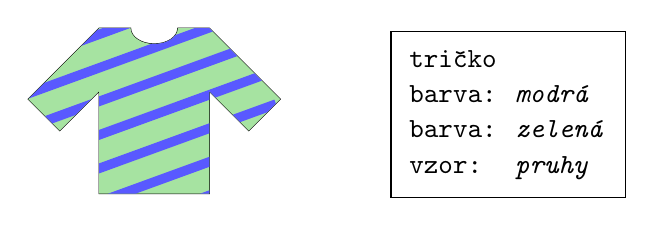
\begin{tikzpicture}
		\definecolor{green1}{HTML}{A6E3A1}
		\begin{scope}
			\draw[clip] (0,-1) -- ++(0.7,0) -- ++(0,1.3) -- ++(0.5,-0.5) -- ++(0.4,0.4) -- ++(-0.9,0.9) -- ++(-0.4,0)
			arc[start angle=0,end angle=-180,x radius=0.3, y radius=0.2]
			-- ++(-0.4,0) -- ++(-0.9,-0.9) -- ++(0.4,-0.4) -- ++(0.5,0.5) -- ++(0,-1.3) -- cycle;
			\begin{scope}[rotate=20]
				\draw[fill=green1,draw=none] (0,0) circle (2);
				\foreach \n in {0, 1, ..., 10}{
						\node[transform shape,scale=0.3,fill=blue!65,draw=none,minimum width=10cm, minimum height=4mm] at (0,-2+\n*0.4) {};
					}
			\end{scope}
		\end{scope}
		\matrix[draw, anchor=west] at (3, 0) {
			\node  {\texttt{\textbf{tričko}}};  \\
			\node {\texttt{barva:}}; &
			\node {\texttt{\textit{modrá}}};   \\
			\node {\texttt{barva:}}; &
			\node {\texttt{\textit{zelená}}};   \\
			\node {\texttt{vzor:}}; &
			\node {\texttt{\textit{pruhy}}};   \\
		};
	\end{tikzpicture}
	\caption{Příklad použití atributů pro popis objektu}\label{fig:example_tshirt}
\end{figure}

Pro složitější objekty se opět naskýtá problém toho, jaké vlastnosti vybrat a zapsat do referenčního popisu, a které je možné naopak zanedbat.
Tato otázka je podobná problematice nejednoznačnosti, zmíněné v části~\ref{subsubsec:objekty_ve_scene} definující objekty.
A i zde platí to, že popis byl záměrně vytvořen tak, aby byl univerzální a volba atributů do referenčního popisu
závisí na expertovi a konkrétní aplikaci.


\subsubsection{Vazby mezi objekty}
Dalším typem informace, kterou by měl být referenční popis obrázku schopen zachytit, jsou vazby a vztahy mezi různými objekty.
Může se jednat například o činnosti, které se týkají dvou objektů, nebo popis relativních vlastností, jako je velikost či pozice.

Každý takový záznam je označen jako \emph{triplet} a skládá se ze \emph{zdrojového objektu},
\emph{cílového objektu} a \emph{predikátu}, který popisuje danou vazbu nebo vztah.
Tato struktura je inspirována běžným zápisem sémantických sítí a RDF standardem~\cite{rdf}.
Obecné schéma jednoho tripletu je na Obrázku~\ref{fig:schema_tripletu}.

\begin{figure}[H]
	\centering
	\begin{tikzpicture}
		\node[draw, ellipse] (n1) at (0,0) {\texttt{zdrojový objekt}};
		\node[draw, ellipse] (n2) at (7,0) {\texttt{cílový objekt}};
		\draw[-Stealth] (n1) to node[midway, above] {\texttt{predikát}} (n2);
	\end{tikzpicture}
	\caption{Obecné schéma tripletu}\label{fig:schema_tripletu}
\end{figure}

Každý objekt může být součástí libovolného počtu tripletů a to jak v pozici zdrojového, tak cílového objektu.
Objekt také nemusí být součástí žádných vazeb a dokonce v celém popisu nemusí být žádné vazby definované.
Například pokud bychom chtěli pouze testovat paměť uživatele, mohli bychom mu ukázat obrázek, pak jej skrýt a sledovat, jaké objekty si vybaví.
V takové úloze nás vazby mezi objekty vůbec nemusejí zajímat a je tedy zbytečné, aby byly součástí referenčního popisu.

Při vytváření referenčního popisu obrázku se opět naskýtá otázka, jaké vazby a vztahy mezi objekty do popisu zavést, a které lze ignorovat.
Například relativní velikost nebo pozice objektů může být pro některé úlohy klíčová, ale pro jiné zcela nepodstatná.
Tato problematika byla opět ponechána na expertovi, který vytváří referenční popis pro danou konkrétní aplikaci,
aby rozhodl, které informace je potřeba v referenčním popise zachytit.

Konkrétní příklad několika tripletů je znázorněn na Obrázku~\ref{fig:triplety_priklad}.
\begin{figure}[H]
	\centering
	\begin{tikzpicture}
		\node[draw] at (-5, 1) {
\includegraphics[scale=0.35]{imgs/dog_squirrel_tree_mushroom.pdf}};
		\node[draw, ellipse, minimum width=1.5cm, minimum height=1cm] (dog) at (0,0) {\texttt{pes}};
		\node[draw, ellipse, minimum width=2cm, minimum height=1cm] (sq) at (5,0) {\texttt{veverka}};
		\node[draw, ellipse, minimum width=2cm, minimum height=1cm] (tree) at (2,3) {\texttt{strom}};
		\node[draw, ellipse, minimum width=2cm, minimum height=1cm] (mush) at (5.5,3) {\texttt{houba}};
		\draw[-Stealth, bend left=25] (dog) to node[midway, above] {\footnotesize \texttt{běží za}} (sq);
		\draw[-Stealth] (dog) to node[midway, above] {\footnotesize \texttt{větší než}} (sq);
		\draw[-Stealth, bend left=25] (sq) to node[midway, below] {\footnotesize \texttt{utíká před}} (dog);
		\draw[-Stealth] (sq) -- node[midway, above, sloped] {\footnotesize \texttt{šplhá na}} (tree);
		\draw[-Stealth] (mush) -- node[midway, above, sloped] {\footnotesize \texttt{je pod}} (tree);
		\draw[-Stealth, bend left=30] (mush) -- node[midway, above, sloped] {\footnotesize \texttt{větší než}} (sq);
		\draw[-Stealth] (dog) to node[midway, above, sloped] {\footnotesize \texttt{je pod}} (tree);
	\end{tikzpicture}
	\caption{Příklad použití tripletů pro popis vztahů mezi objekty}\label{fig:triplety_priklad}
\end{figure}

\subsubsection{Další typy informací}
Kromě výše zmíněných objektů, jejich vlastností a vazeb, je také možné pro některé aplikace požadovat,
aby byly zachyceny i další jiné informace.

Jednou takovou dodatečnou informací může být například přesah zobrazené scény do reálného života, nebo extrapolace dějů a objektů.
Tím jsou myšlené různé další objekty, děje, činnosti nebo vlastnosti, které nejsou
přímo zobrazené na daném obrázku, ale z kontextu by bylo možné je nějakým způsobem předvídat.
Příkladem takové situace může být ilustrace zobrazující například dítě, které si hraje blízko břehu řeky - v takovém případě je možné
požadovat zachycení informace ve stylu \enquote{dítě může spadnout do vody}.

Druhým typem dodatečné informace může být meta-popis samotné scény.
Pod tímto pojmem jsou myšlené obecné informace o obrázku, například celkový popis toho, co je na scéně vyobrazeno.
Například pro Obrázek~\ref{fig:summer} by mohl být takovýmto meta-popisem například \enquote{scéna na břehu rybníka}.

Pro oba tyto typy informací nebyly navrženy žádné speciální datové struktury.
Bylo rozhodnuto, že v případě potřeby je možné tyto informace zachytit dostatečně dobře pomocí již definovaných
objektů, atributů a vazeb mezi objekty.

Případné rozšíření formy referenčního popisu o nějaké další specializované typy popisů bylo ponecháno jako předmět dalšího budoucího možného rozšíření.

\newpage
\subsection{Extrakce sémantické informace}\label{subsec:extrakce_semanticke_informace}
Dalším klíčovým bodem bylo najít způsob, jak porovnat uživatelský popis obrázku s jeho referenčním popisem.
To je úlohou subsystému pro získání sémantické informace z textu.
Cílem je z přirozené řeči extrahovat informace v takové podobě, aby je bylo možné porovnat se strukturovaným referenčním popisem.

% Dalším klíčovým bodem při návrhu systému pro hodnocení popisu obrázku bylo najít způsob, jak z získat požadovanou sémantickou informaci.
% Cílem je z přirozené lidské řeči extrahovat informace v takové podobě, aby je bylo možné porovnat s naším referenčním popisem obrázku a
% následně vyhodnotit jejich podobnost.

Extrakce sémantiky z přirozené řeči se běžně dělá z textového přepisu dané promluvy.
\todo{ozdrojovat!}
I v této práci tedy extrakce sémantických informací probíhá z textu.
To znamená, že pokud uživatel popíše obrázek mluvenou řečí, tak je potřeba promluvu převést do textu pomocí nějakého systému pro rozpoznání řeči.
Problematika rozpoznání řeči a převodu audia do textu je nad rámec této práce a bude v praxi řešena nějakou již existující implementací.
Ve zbytku práce bude tedy pro zjednodušení rovnou uvažovaným vstupem text.

Otázka extrakce sémantické informace z popisu přirozenou řečí se tedy zužuje na extrakci sémantiky z textu.
Jako způsob řešení byl zvolen přístup založený na sémantickém parsování pomocí bezkontextových gramatik.

Tento přístup funguje tak, že na základě referenčního popisu obrázku bude expertem sestavena gramatika,
podle které budou v textu detekované jednotlivé části sémantické informace.
Gramatika je v tomto kontextu sada pravidel, která definují, jaké promluvy jsou v textu očekávané a jak mohou tyto promluvy vypadat.
Program pak tato pravidla načte a prochází podle nich vstupní text a hledá, zda nějaké části textu \enquote{pasují} na dané pravidlo.
Samotný nalezený kus textu, který \enquote{pasuje} na nějaké pravidlo, ale ještě nemá žádný užitečný význam.
Proto pravidla obsahují zároveň i informaci o tom, jaká je struktura nalezené části textu a jaký význam mají jednotlivé části této struktury.
V českém jazyce by se jednalo o obdobu větného rozboru, kdy se například určuje, která část věty je podmět a která přísudek.

Strukturovaná a označkovaná část textu s doplněnou sémantickou informací je pak označována jako \emph{sémantická entita}.
Konkrétní syntaxe, použití a funkčnost těchto gramatik bude popsán později spolu s implementací v části~\ref{subsec:moje_gramatiky}.
Množina všech těchto sémantických entit, které byly ze vstupního textu extrahované, jsou pak použité pro vytvoření testovaného popisu.

\subsubsection{Podoba sémantických entit}
První otázkou, kterou bylo potřeba vyřešit pro získání sémantické informace z přirozeného popisu, byla její podoba.
Jinými slovy, jak by měla extrahovaná sémantika vypadat, aby ji bylo možné porovnat s referenčním popisem obrázku.

Vzhledem k tomu, že výše definovaný referenční popis (viz sekce~\ref{subsec:reprezentace_znalosti}) se skládá z objektů, jejich hierarchie, atributů a vazeb,
tak se nabízí přímo použít tyto typy informací.
Bylo tedy rozhodnuto, že z přepisu přirozené řeči budou extrahované objekty, jejich atributy a vazby mezi nimi.

\subsubsection{Extrakce sémantiky - objekty}
Základním typem informace, kterou musí být systém schopen z přepisu řeči získat, jsou samotné objekty, které expert definoval v referenčním popisu obrázku.

Například ze vstupní promluvy
\begin{center}
	\enquote{\emph{Na obrázku vidím psa s veverkou, strom a nějakou houbu.}}
\end{center}
by měl systém vrátit množinu detekovaných objektů $\mathcal{O}$:
\[
	\mathcal O = \bigl\{\, \texttt{pes}, \texttt{veverka}, \texttt{strom}, \texttt{houba}\, \bigr\}
\]
Ve své nejjednodušší podobě by se mohlo jednat pouze o detekci nějakých klíčových slov, které odpovídají názvům objektů.
Skutečná realizace je poněkud složitější, bere v potaz různá synonyma, tvary slov a alternativní vyjádření.
% Stejně jako zbytek SLU subsystému je založená na pravidlech bezkontextové gramatiky.
% Pomocí těchto pravidel lze specifikovat, jaké jsou očekávané vyjádření jednotlivých objektů ve scéně.
Detailněji bude popsána později spolu s konkrétní implementací v kapitole~\ref{sec:implementace}.

% Složitost detekce objektů plyne především z toho, že český jazyk je velmi bohatý na synonyma a různé tvary slov.
% To znamená, že jeden objekt může být popsaný různými lidmi zcela odlišnými slovy a nebo i jeden člověk může stejnou věc vyjádřit pokaždé jinak.
% Také záleží na kontextu daného slova, který může ovlivnit jeho konkrétní tvar.

Detekce samotných objektů by mohla být pro některé aplikace dokonce postačující sama o sobě.
Mohlo by se jednat o úlohy, kde je hlavním předmětem pouze zjistit, kolik objektů na obrázku člověk popíše, případně které to jsou.
Typickými příklady by mohli být nějaké testy paměti, pozornosti nebo jednoduché klasifikace.

\newpage
\subsubsection{Extrakce sémantiky - atributy}
Druhým typem sémantické informace, kterou je potřeba, aby byl systém schopen najít a extrahovat z textu, jsou atributy popisující vlastnosti objektů.

Ve srovnání s detekcí samotných objektů se jedná o značně složitější problém, protože pro extrakci atributu je potřeba mít informace o objektu,
na který se atribut váže, o názvu daného atributu a také o jeho přiřazené hodnotě.

Například ve větě
\begin{center}
	\enquote{\emph{Na obrázku vidím kluka v modrém tričku.}}
\end{center}
by měl systém detekovat, že objekt \enquote{\texttt{tričko}} má atribut \enquote{\texttt{barva}} s hodnotou \enquote{\texttt{modrá}}.

Kromě toho, že se tato informace skládá z více nezávislých částí, tak je možné si všimnout, že se ve zdrojové větě nikde nevyskytuje slovo \enquote{\emph{barva}}.
Toto je tedy informace, kterou musí být systém schopen nějakým způsobem indukovat z okolních dat a referenčního popisu.

Dále by jiný uživatel mohl popsat stejný obrázek třeba větou
\begin{center}
	\enquote{\emph{Vidím nějakého kluka v tričku, které je modré}}.
\end{center}
Tato promluva obsahuje stejný objekt, atribut i hodnotu, ale vyjádřenou ve zcela jiné podobě.
Jak je tedy zřejmé, zde již není možné použít pouze nějakou formu detekce klíčových slov, ale bude potřeba komplikovanějšího přístupu.

Právě dříve zmíněná pravidla, která udávají různé formy hledané informace, umožňují zachytit i takovéto složitější struktury v různých formách.
Konkrétní realizace bude opět popsána později, viz sekce~\ref{sec:implementace}.

\newpage
\subsubsection{Extrakce sémantiky - vazby mezi objekty}
Posledním typem informace, kterou je potřeba získat z textu, jsou vazby mezi objekty.

Například pro větu
\begin{center}
	\enquote{\emph{Na obrázku hnědého vidím psa, co běží za oranžovou veverkou.}}
\end{center}
je třeba, aby systém dokázal detekovat vazbu mezi objektem psa a veverky:
\begin{center}
	\begin{tikzpicture}
		\node[draw, rounded corners=3mm, minimum height=7mm, minimum width=1cm] (n1) at (0, 0) {\texttt{pes\vphantom{k}}};
		\node[draw, rounded corners=3mm, minimum height=7mm, minimum width=1.8cm] (n2) at (4, 0) {\texttt{veverka\vphantom{p}}};
		\draw[-Stealth] (n1) -- node[midway, above] {\texttt{běží za}} (n2);
	\end{tikzpicture}
\end{center}

Jak je zřejmé, pro sestavení vazby je - stejně jako pro atributy - potřeba tří částí informace: zdrojový objekt, cílový objekt a název vazby.
Na rozdíl od detekce atributů ale představuje detekce vazeb unikátní problém, protože zdrojový a cílový objekt jsou stejného typu - oba jsou to objekty.
To znamená, že v při konstrukci tripletů musí být použit nějaký mechanismus, který rozpozná, který z objektů má být cílový a který zdrojový.
Tento problém je řešen také v rámci definice pravidel v bezkontextové gramatice pomocí tagů, detailní popis v sekci~\ref{subsec:moje_gramatiky}.

Je vhodné zmínit, že ačkoli byly v kapitole~\ref{subsec:reprezentace_znalosti} definované čtyři aspekty popisu,
nyní jsou řešené pouze tři různé typy sémantických entit.
To je proto, že hierarchie mezi objekty byla při návrhu považována za speciální případ vazby mezi objekty a nebyla pro ni vytvořena samostatná kategorie.

\newpage
\subsection{Hodnotící algoritmus}\label{subsec:hodnoceni}
Za předpokladu, že je k dispozici referenční popis vytvořený expertem a testovaný popis získaný automaticky z přirozené řeči,
je potřeba tyto dva popisy nějakým způsobem porovnat a určit, do jaké míry odpovídá testovaný popis referenčnímu.

Právě to je předmětem této kapitoly: navrhnout algoritmus, který by zajišťoval porovnání testovaného popisu s referenčním a jehož výstupem by bylo nějaké hodnocení.

Základ hodnotícího algoritmu vychází ze struktury referenčního a testovaného popisu.
Oba typy se skládají z množiny objektů $\mathcal O$, množiny atributů $\mathcal A$ a množiny vazeb $\mathcal V$.
Dolním indexem je značeno, zda se jedná o množinu z referenčního popisu ($R$), nebo testovaného popisu ($T$).
Oba popisy obrázku lze tedy vyjádřit jako trojice:
\begin{align*}
	\text{\emph{referenční popis obrázku}} & = \bigl( \mathcal{O}_{R}, \mathcal{A}_{R}, \mathcal{V}_{R} \bigr), \\
	\text{\emph{testovaný popis obrázku}}  & = \bigl( \mathcal{O}_{T}, \mathcal{A}_{T}, \mathcal{V}_{T} \bigr).
\end{align*}
Porovnání a hodnocení podobnosti popisů by tak mohlo být převedeno na otázku porovnání podobnosti množin.
Otázky teorie množin jsou ale nad rámec zadání a pro tuto práci byl definován hodnotící algoritmus,
který je inspirován ztrátovými funkcemi.

Na obecné úrovni by se dalo říci, že hodnotící algoritmus počítá celkové ztráty pro chybějící objekty,
chybějící atributy, atributy s chybnou hodnotou, chybějící vazby mezi objekty.

Vstupem hodnotícího algoritmu jsou tedy oba popisy (referenční a testovaný) a k tomu ještě ztrátová tabulka,
která určuje, jaký typ chyby způsobí jak velkou ztrátu.
Tuto ztrátovou tabulku také sestavuje expert, společně s referenčním popisem.

Výstupem hodnotícího algoritmu je pak množina označených číselných hodnot, které reprezentují celkové ztráty pro různé druhy chyb.

\subsubsection{Chybějící objekty}
Pokud byl v~referenčním popisu expertem označený nějaký objekt,
který chybí v~testovaném popise, předpokládá se, že expert považoval daný objekt za důležitý a uživatel jej nezmínil.

Uživatel si třeba nemusel objektu všimnout, nebo jej nepovažoval za dostatečně důležitý.
V obou případech se však jedná o nějaký rozpor se vzorovým popisem, který je třeba penalizovat.

Například pro situaci:
\begin{align*}
	\mathcal{O}_{R} & = \bigl\{\, \texttt{pes}, \texttt{veverka}, \texttt{houba}, \texttt{strom}\, \bigr\} \\
	\mathcal{O}_{T} & = \bigl\{\, \texttt{pes}, \texttt{veverka}\, \bigr\}
\end{align*}
je zřejmé, že v testovaném popisu chybí dva objekty: \texttt{houba} a \texttt{strom}.

Lze očekávat, že různé objekty budou ve scéně různě důležité a bylo by vhodné, aby byl tento fakt zohledněn při výpočtu ztráty.
Proto lze přiřadit objektům \emph{tagy}.
Jako \emph{tag} je v tomto kontextu chápána nějaká značka, která říká, že objekt patří do dané skupiny.
Například objekt \enquote{\texttt{tričko}} může mít přiřazen tag \enquote{\emph{oblečení}} a objekt \enquote{\texttt{pes}}
může mít přiřazen tag \enquote{\emph{zvíře}}.

Pro větší variabilitu systému bylo dále rozhodnuto, že každý objekt může mít přiřazený libovolný počet tagů.
Název tagů a jejich přiřazení objektům je volbou experta a je součástí tvorby referenčního popisu.
Ve ztrátové tabulce pak může expert definovat ztrátové hodnoty pro jednotlivé tagy a tím tak přepsat hodnotu ztráty na daném objektu.

Pokud má objekt přiřazeno více tagů, na jejich pořadí záleží.
Při určování ztrátové hodnoty pro daný objekt algoritmus postupně prochází jeden tag po druhém a kontroluje, zda je tento tag uvedený ve ztrátové tabulce.
Pokud ano, je ztráta na daném jednom chybějícím objektu rovna této hodnotě a další tagy na tomto objektu již nejsou kontrolované.
Pokud žádný z tagů není nalezen ve ztrátové tabulce, je použita výchozí hodnota ztráty pro jakýkoli chybějící objekt.

Pro názornost je schéma jednoho ukázkového případu na Obrázku~\ref{fig:example_missing_objects}.

\def\objone{míč}
\def\objtwo{chleba}
\def\objthree{pes}
\def\objfour{strom}
\def\objfive{kuře}
\def\objsix{mrkev}
\def\objseven{jahoda}
\def\objeight{kapr}
\def\tagone{jídlo}
\def\tagtwo{zvíře}
\def\tagthree{rostlina}

\begin{figure}[H]
	\centering
	\begin{tikzpicture}
		\node[draw, minimum width=4cm, minimum height=2cm] (comp) at (0, 0) {\parbox{3cm}{\small \centering výpočet ztráty pro chybějící objekty}};
		\node[anchor=west, inner sep=0mm] (out) at ($(comp.east) + (2.5, 0)$) {
			\small
			\centering
			\begin{tabular}{|c|c|}
				\hline
				\textbf{Objekt} & \textbf{Ztráta} \\
				\hline
				{\objone}       & 1.0             \\
				{\objtwo}       & 0.5             \\
				{\objthree}     & 1.0             \\
				{\objfour}      & 0.0             \\
				{\objfive}      & 0.5             \\
				{\objsix}       & 0.5             \\
				{\objseven}     & 3.0             \\
				{\objeight}     & 0.0             \\
				\hline
			\end{tabular}
		};
		\node[anchor=south, inner sep=0mm] (ztr) at ($(comp.north) + (0, 1)$) {
			\small
			\centering
			\begin{tabular}{|c|c|}
				\hline
				\textbf{Typ}   & \textbf{Ztráta} \\
				\hline
				\emph{výchozí} & 1.0             \\
				{\tagone}      & 0.5             \\
				{\tagthree}    & 3.0             \\
				\hline
			\end{tabular}
		};
		\node[anchor=south east, inner sep=0mm] (ref) at ($(comp.west) + (-1, 1)$) {
			\small
			\centering
			\begin{tabular}{|c|c|}
				\hline
				\textbf{Objekt} & \textbf{Tagy}          \\
				\hline
				{\objone}       & --                     \\
				{\objtwo}       & {\tagone}              \\
				{\objthree}     & {\tagtwo}              \\
				{\objfour}      & {\tagthree}            \\
				{\objfive}      & {\tagone}, {\tagtwo}   \\
				{\objsix}       & {\tagone}, {\tagthree} \\
				{\objseven}     & {\tagthree}, {\tagone} \\
				{\objeight}     & {\tagtwo}, {\tagone}   \\
				\hline
			\end{tabular}
		};
		\draw[-Stealth, rounded corners=2mm] (ref.south) |- node[near end, above] {\scriptsize referenční popis} ($(comp.west) + (0, 0.2)$);
		\draw[-Stealth] (ztr.south) -- node[midway, right] {\scriptsize ztrátová tabulka} (comp.north);
		\draw[-Stealth] (comp) -- node[midway, above] {\scriptsize vypočtené ztráty} (out);
		\node[draw] (in2) at ($(ref.south) + (0, -2.5)$) {$\mathcal{O}_{T} = \bigl\{ \, \objfour, \objeight \, \bigr\}$};
		\draw[-Stealth, rounded corners=2mm] (in2.north) |- node[near end, below] {\scriptsize testovaný popis} ($(comp.west) + (0, -0.2)$);
	\end{tikzpicture}
	\caption{Jednoduchá ukázka ztráty na chybějících objektech}\label{fig:example_missing_objects}
\end{figure}

Na příkladu zobrazeném na Obrázku~\ref{fig:example_missing_objects} je možné vidět, že objekt \emph{\objfour},
který byl nalezený v testovaném popisu, nezpůsobil žádnou ztrátu.
Ostatní objekty, které v testovaném popise chybí, způsobily ztrátu odpovídající hodnotě ze ztrátové tabulky.
Dále je možné si všimnout, že objekty \emph{\objsix} a \emph{\objseven} mají stejné tagy, ale v jiném pořadí, proto jsou jimi způsobené ztráty rozdílné.

Pro větší kompaktnost výstupu nejsou vypočtené ztráty prezentované pro každý objekt samostatně, ale jsou sečtené do finálního výsledku.
Tento proces sčítání ztrátových hodnot je přes všechny objekty, ale také jsou počítané hodnoty přes jednotlivé tagy.
Pokud bychom vzali tabulku vypočtených ztrát pro jednotlivé objekty z příkladu na Obrázku~\ref{fig:example_missing_objects},
šel by tento finální krok znázornit Obrázkem~\ref{fig:example_missing_objects_final_sum}.

\begin{figure}[ht!]
	\centering
	\begin{tikzpicture}
		\node[anchor=west, inner sep=0mm] (in) at (0, 0) {
			\small
			\centering
			\begin{tabular}{|c|c|c|}
				\hline
				\textbf{Objekt} & \textbf{Tagy}          & \textbf{Ztráta} \\
				\hline
				{\objone}       & ---                    & 1.0             \\
				{\objtwo}       & {\tagone}              & 0.5             \\
				{\objthree}     & {\tagtwo}              & 1.0             \\
				{\objfour}      & {\tagthree}            & 0.0             \\
				{\objfive}      & {\tagone}, {\tagtwo}   & 0.5             \\
				{\objsix}       & {\tagone}, {\tagthree} & 0.5             \\
				{\objseven}     & {\tagthree}, {\tagone} & 3.0             \\
				{\objeight}     & {\tagtwo}, {\tagone}   & 0.0             \\
				\hline
			\end{tabular}
		};
		\node[anchor=west, inner sep=0mm] (out) at (7, 0) {
			\small
			\centering
			\begin{tabular}{|l|c|}
				\hline
				\textbf{Chybějící objekty}    & \textbf{Ztráta} \\
				\hline
				všechny                       & 6.5             \\
				objekty s \enquote{\tagone}   & 4.5             \\
				objekty s \enquote{\tagtwo}   & 1.5             \\
				objekty s \enquote{\tagthree} & 3.5             \\
				\hline
			\end{tabular}
		};
		\draw[-Stealth] ($(in.east) + (0.3, 0)$) -- node[midway, above] {\scriptsize sečtení} ($(out.west) + (-0.3, 0)$);
	\end{tikzpicture}
	\caption{Finálního krok při počítání ztrát na chybějících objektech}\label{fig:example_missing_objects_final_sum}
\end{figure}

Zde je vhodné zmínit, že popsaný algoritmus výpočtu ztráty je pouze jednou z možností.
Pro konkrétní nasazení by mohla být vhodnější jiná forma počítání ztrátových hodnot,
například vypočítat průměr, sumu nebo maximum či minimum.
Tento způsob počítání ztráty byl zvolen proto, že poskytuje expertovi další stupeň volnosti,
jak vyjádřit důležitost objektů.

\newpage
\subsubsection{Chybějící atributy}
Pokud expert popsal na daném objektu nějakou vlastnost a odpovídající atribut chybí v~testovaném popise,
je zde stejný předpoklad jako u~chybějících objektů, a~také se jedná o chybu, která způsobí navýšení ztrátové hodnoty.

Způsob hodnocení je obdobný jako pro chybějící objekty, pouze s tím rozdílem, že atributům nejsou přiřazovány žádné tagy.
Tagy u objektů sloužily k detailnějšímu určení důležitosti objektu a později ke sčítání ztrátových hodnot,
v případě atributů tuto funkci zastává samotný název atributu.

Například pokud by byl libovolný chybějící atributu penalizován ztrátou $1.0$, pak by bylo možné
specifikovat, že vynechání atributu \emph{\enquote{barva}} je méně závažné než všechny ostatní a penalizovat pouze ztrátou $0.5$.
Naopak vynechání atributu \emph{\enquote{výraz v obličeji}} (např.~úsměv nebo zamračení) by mohl být považován za důležitý a expert by
mohl ve~ztrátové tabulce definovat, že jeho vynechání bude penalizováno ztrátou $2.0$.

Jednoduchý příklad je znázorněn na Obrázku~\ref{fig:example_missing_attrs}.

\begin{figure}[H]
	\centering
	\begin{tikzpicture}
		\node[draw, minimum width=4cm, minimum height=2cm] (comp) at (0, 0) {\parbox{3cm}{\small \centering výpočet ztráty pro chybějící atributy}};
		\node[anchor=west, inner sep=0mm] (out) at ($(comp.east) + (0, -3.5)$) {
			\small
			\centering
			\begin{tabular}{|l|c|}
				\hline
				\textbf{Atribut}        & \textbf{Ztráta} \\
				\hline
				míč: barva = modrá      & 0.0             \\
				míč: tvar = kulatý      & 2.0             \\
				míč: typ = fotbalový    & 1.0             \\
				krabice: barva = bílá   & 0.5             \\
				krabice: tvar = hranatý & 0.0             \\
				\hline
			\end{tabular}
		};
		\node[anchor=south, inner sep=0mm] (ztr) at ($(comp.north) + (0, 1)$) {
			\small
			\centering
			\begin{tabular}{|c|c|}
				\hline
				\textbf{Typ atributu} & \textbf{Ztráta} \\
				\hline
				\emph{výchozí}        & 1.0             \\
				{barva}               & 0.5             \\
				{tvar}                & 2.0             \\
				\hline
			\end{tabular}
		};
		\node[anchor=south east, inner sep=0mm] (ref) at ($(comp.west) + (-1, 1)$) {
			\small
			\centering
			\begin{tabular}{|l|}
				\hline
				\textbf{Atributy}       \\
				\hline
				míč: barva = modrá      \\
				míč: tvar = kulatý      \\
				míč: typ = fotbalový    \\
				krabice: barva = bílá   \\
				krabice: tvar = hranatý \\
				\hline
			\end{tabular}
		};
		\draw[-Stealth, rounded corners=2mm] (ref.south) |- node[near end, above] {\scriptsize referenční popis} ($(comp.west) + (0, 0.2)$);
		\draw[-Stealth] (ztr.south) -- node[midway, right] {\scriptsize ztrátová tabulka} (comp.north);
		\draw[-Stealth] (comp) -| node[near start, above] {\scriptsize vypočtené ztráty} (out.north);
		\node[inner sep=0pt] (in2) at ($(ref.south) + (0, -2.5)$) {
			\small
			\centering
			\begin{tabular}{|l|}
				\hline
				míč: barva = modrá      \\
				krabice: tvar = hranatý \\
				\hline
			\end{tabular}
		};
		\draw[-Stealth, rounded corners=2mm] (in2.north) |- node[near end, below] {\scriptsize testovaný popis} ($(comp.west) + (0, -0.2)$);
	\end{tikzpicture}
	\caption{Ukázka výpočtu ztrát pro chybějící atributy}\label{fig:example_missing_attrs}
\end{figure}

\subsubsection{Chybějící vazby mezi objekty}
Posledním typem entity, která může chybět při porovnávání referenčního a testovaného popisu, jsou vazby mezi objekty popsané \emph{triplety}.

Zde je hodnotící algoritmus velmi podobný jako při počítání ztráty pro chybějící objekty.
Rozdíl zde spočívá v tom, že místo tagů jsou zde použité samotné názvy vazeb, podobně jako u chybějících atributů jsou použité názvy atributů.

Expert ve ztrátové tabulce opět specifikuje, jaká je výchozí hodnota ztráty, pokud v testovaném popise bude chybět libovolná vazba mezi objekty.
Následně může také specifikovat, že některé konkrétní typy vazeb (podle jejich názvu) mají větší či menší důležitost a tak jimi způsobená ztráta může být větší nebo menší.
Algoritmus pak při výpočtu použije přednostně takovou hodnotu, která je více specifická.

Konkrétní příklad je znázorněn na Obrázku~\ref{fig:example_missing_triplets}.

\begin{figure}[H]
	\centering
	\begin{tikzpicture}
		\node[draw, minimum width=4cm, minimum height=2cm] (comp) at (0, 0) {\parbox{3cm}{\small \centering výpočet ztráty pro chybějící vazby}};
		\node[anchor=west, inner sep=0mm] (out) at ($(comp.east) + (-2, -4)$) {
			\small
			\centering
			\begin{tabular}{|l|c|}
				\hline
				\textbf{Vazba mezi objekty}      & \textbf{Ztráta} \\
				\hline
				pes \to\ běží za \to\ veverka    & 0.0             \\
				veverka \to\ utíká před \to\ pes & 1.0             \\
				pes \to\ je pod \to\ strom       & 1.0             \\
				pes \to\ větší než \to\ veverka  & 0.5             \\
				veverka \to\ šplhá na \to\ strom & 0.0             \\
				\hline
			\end{tabular}
		};
		\node[anchor=south, inner sep=0mm] (ztr) at ($(comp.north) + (0, 1)$) {
			\small
			\centering
			\begin{tabular}{|c|c|}
				\hline
				\textbf{Název vazby} & \textbf{Ztráta} \\
				\hline
				\emph{výchozí}       & 1.0             \\
				{větší než}          & 0.5             \\
				{běží za}            & 2.0             \\
				\hline
			\end{tabular}
		};
		\node[anchor=south east, inner sep=0mm] (ref) at ($(comp.west) + (-1, 1)$) {
			\small
			\centering
			\begin{tabular}{|l|}
				\hline
				\textbf{Vazby mezi objekty}      \\
				\hline
				pes \to\ běží za \to\ veverka    \\
				veverka \to\ utíká před \to\ pes \\
				pes \to\ je pod \to\ strom       \\
				pes \to\ větší než \to\ veverka  \\
				veverka \to\ šplhá na \to\ strom \\
				\hline
			\end{tabular}
		};
		\draw[-Stealth, rounded corners=2mm] (ref.south) |- node[near end, above] {\scriptsize referenční popis} ($(comp.west) + (0, 0.2)$);
		\draw[-Stealth] (ztr.south) -- node[midway, right] {\scriptsize ztrátová tabulka} (comp.north);
		\draw[-Stealth] (comp) -| node[at start, above, anchor=south west] {\scriptsize vypočtené ztráty} (out.north);
		\node[inner sep=0pt] (in2) at ($(ref.south) + (0, -2.5)$) {
			\small
			\centering
			\begin{tabular}{|l|}
				\hline
				pes \to\ běží za \to\ veverka    \\
				veverka \to\ šplhá na \to\ strom \\
				\hline
			\end{tabular}
		};
		\draw[-Stealth, rounded corners=2mm] (in2.north) |- node[near end, below] {\scriptsize testovaný popis} ($(comp.west) + (0, -0.2)$);
	\end{tikzpicture}
	\caption{Ukázka výpočtu ztrát pro chybějící vazby mezi objekty}\label{fig:example_missing_triplets}
\end{figure}

\subsubsection{Atributy s chybnou hodnotou}
Pokud byl v testovém popise nalezen atribut, který odpovídá objektem a názvem nějakému atributu z referenčního popisu,
ale neodpovídá svou hodnotou žádnému referenčnímu atributu, pak se předpokládá, že uživatel udělal chybu při popisu a řekl špatnou hodnotu.

Příkladem takové neshody by mohlo být:
\begin{align*}
	\mathcal{A}_{R} & = \bigl\{ \, \texttt{tričko: barva = modrá } \, \bigr\}, \\
	\mathcal{A}_{T} & = \bigl\{ \, \texttt{tričko: barva = zelená} \, \bigr\},
\end{align*}
pak je možné předpokládat, že uživatel udělal při popisu chybu a řekl špatnou barvu.

Způsob počítání ztrátové hodnoty z těchto chybných hodnot je v principu stejný jako u chybějících objektů a atributů.
Expert ve ztrátové tabulce definuje výchozí hodnotu a~k~tomu případně specifické případy, kdy je tato ztrátová hodnota jiná.

% Expert ve ztrátové tabulce definuje, jaká je výchozí ztráta pro chybně určenou hodnotu atributu a případně jaké konkrétní situace tuto hodnotu přepisují na jinou.
Rozdíl oproti předchozím výpočtům ovšem spočívá v tom, že různé hodnoty si mohou být různě blízko.
Například pokud uživatel zamění hnědou a oranžovou barvu veverky, tak se pravděpodobně ve většině případů bude jednat o menší chybu,
než kdyby oranžovou zaměnil třeba za zelenou.

Z toho důvodu je ztrátová tabulka navržena tak, aby expert mohl definovat výchozí ztrátu pro všechny chybné atributy,
výchozí ztrátu pro konkrétní atribut bez ohledu na hodnoty, ztrátu pro konkrétní atribut a zároveň množinu konkrétních hodnot, jejichž záměna tuto ztrátu způsobí.

Pro lepší názornost následuje příklad, který předpokládá, že expert definoval ztrátovou tabulku shodnou s Tabulkou~\ref{tab:example_wrong_attrs_values}.
Tu je možné číst následujícím způsobem:
\begin{enumerate}
	\item Libovolný chybný atribut způsobí ztrátu 1.0, pokud není ve zbytku tabulky definována více specifická alternativa.
	\item Pokud je chybná hodnota v atributu \enquote{\texttt{barva}}, pak je způsobená ztráta rovna 0.5, pokud se nejedná o záměnu některých konkrétních hodnot:
	      \begin{itemize}
		      \item Pokud je zaměněna barva \enquote{\texttt{žlutá}} a \enquote{\texttt{oranžová}}, pak je ztráta 0.3.
		      \item Pokud je zaměněna barva \enquote{\texttt{červená}}, \enquote{\texttt{modrá}} nebo \enquote{\texttt{zelená}} (libovolná dvojice), pak je ztráta rovna 0.8.
	      \end{itemize}
	\item Pokud je chybná hodnota v atributu \enquote{\texttt{tvar}}, pak je ztráta 1.5.
\end{enumerate}
Ukázka některých konkrétních atributů s chybnými hodnotami a k nim vypočtených ztrát je zobrazena v Tabulce~\ref{tab:example_wrong_attrs_table}.

\begin{figure}[H]
	\centering
	\begin{tikzpicture}[remember picture]
		\node[] (base) at (0, 0) {
			\begin{tabular}{|c|c|}
				\hline
				\textbf{Atribut} & \textbf{Ztráta} \\
				\hline
				\emph{výchozí}   & 1.0             \\
				\hline
				\texttt{barva}   &                 \\
				\hline
				\texttt{tvar}    &                 \\
				\hline
			\end{tabular}
		};
		\node[circle, fill=black, scale=0.4] (n1) at ($(base.south east) + (-0.95, 0.47)$) {};
		\node[circle, fill=black, scale=0.4] (n2) at ($(base.south east) + (-0.95, 1.15)$) {};
		\node[anchor=north west] (t1) at ($(base.north east) + (1.5, 0)$) {
			\begin{tabular}{|l|l|}
				\hline
				\textbf{Hodnoty}                                  & \textbf{Ztráta} \\
				\hline
				\emph{výchozí}                                    & 0.5             \\
				\texttt{žlutá}, \texttt{oranžová}                 & 0.3             \\
				\texttt{červená}, \texttt{modrá}, \texttt{zelená} & 0.8             \\
				\hline
			\end{tabular}
		};
		\node[anchor=north west] (t2) at ($(t1.south west) + (0, -0.5)$) {
			\begin{tabular}{|l|l|}
				\hline
				\textbf{Hodnoty} & \textbf{Ztráta} \\
				\hline
				\emph{výchozí}   & 1.5             \\
				\hline
			\end{tabular}
		};
		\draw[-Stealth] (n2) to (t1.west|-n2);
		\draw[-Stealth] (n1) |- (t2.west);
	\end{tikzpicture}
	\caption{Část ukázkové ztrátové tabulky}\label{tab:example_wrong_attrs_table}
\end{figure}

\begin{table}[H]
	\centering
	\begin{tabular}{|l|l|c|}
		\hline
		\textbf{Referenční atribut}      & \textbf{Testovaný atribut}      & \textbf{Ztráta} \\
		\hline
		\texttt{pes: barva = hnědá}      & \texttt{pes: barva = hnědá}     & 0.0             \\
		\texttt{oheň: barva = žlutá}     & \texttt{oheň: barva = oranžová} & 0.3             \\
		\texttt{jablko: barva = červená} & \texttt{jablko: barva = modrá}  & 0.8             \\
		\texttt{tričko: barva = modrá}   & \texttt{tričko: barva = zelená} & 0.8             \\
		\texttt{čepice: barva = modrá}   & \texttt{čepice: barva = žlutá}  & 0.5             \\
		\texttt{penál: tvar = válec}     & \texttt{penál: tvar = kvádr }   & 1.5             \\
		\texttt{pes: činnost = leží}     & \texttt{pes: činnost = leží }   & 1.0             \\
		\hline
	\end{tabular}
	\caption{Výpočtu ukázkových ztrát chybných hodnot atributů podle Tabulky~\ref{tab:example_wrong_attrs_table}}\label{tab:example_wrong_attrs_values}
\end{table}

Přirozeně se naskýtá otázka toho, jak počítat ztrátu při konfliktu objektů se stejnými atributy a nebo objekty s více atributy.
Pro řešení těchto konfliktů bylo rozhodnuto, že hodnotící algoritmus bude optimistický a bude uvažovat nejmenší možnou chybu,
pokud je podle ztrátové tabulky k dispozici více možných interpretací.

\subsubsection{Výstup hodnotícího algoritmu}
Výstup hodnotícího algoritmu, jak byl popsán v předchozích částech, obsahuje vždy celkovou ztrátu pro daný typ chyby
a poté ještě akumulované ztrátové hodnoty stejného typu, ale rozdělené podle jednotlivých kategorií.

Konkrétně bude výstupní struktura obsahovat:
\begin{itemize}
	\item celkovou ztrátu způsobenou všemi chybějícími objekty,
	\item celkovou ztrátu způsobenou všemi chybějícími atributy,
	\item celkovou ztrátu způsobenou všemi chybějícími vazbami mezi objekty,
	\item celkovou ztrátu způsobenou všemi atributy s chybnými hodnotami,
	\item ztráty způsobené chybějícími objekty s konkrétním tagem,
	\item ztráty způsobené chybějícími atributy s konkrétním názvem/typem atributu,
	\item ztráty způsobené chybějícími vazbami s konkrétním názvem/typem vazby,
	\item ztráty způsobené atributy s chybnými hodnotami, rozdělené podle názvu/typu atributu.
\end{itemize}

Je vhodné zmínit, že při návrhu hodnotícího algoritmu bylo předpokládáno, že pro různá konkrétní nasazení mohou být rozdílné požadavky na formu výstupu.
V rámci implementace popsané později existuje proto \enquote{skrytý} mezi-krok,
ve kterém jsou k dispozici všechny jednotlivé ztráty pro konkrétní objekty, atributy a vazby,
ze kterých je poté počítána právě popsaná výsledná struktura.
Tento mezi-výsledek by bylo možné výhodně využít pro implementaci alternativních způsobů hodnocení, nebo případně rovnou použít jako výstup,
pokud by daná aplikace benefitovala z podrobnější analýzy výsledků.



\clearpage
\section{Implementace a testování}\label{sec:implementace}
V této kapitole je rozebrána konkrétní technická implementace navržených a výše popsaných konceptů a algoritmů.
Jako první bude popsána implementace referenčního popisu obrázku a odpovídající reprezentace znalostí,
následuje popis sémantické analýzy pomocí bezkontextových gramatik a následná tvorba testovaného popisu.
Poté je popsána implementace hodnotícího algoritmu včetně ukázek a na závěr jsou ukázané ilustrační příklady funkčnosti celého systému.

Systém byl vytvořen jako program s ovládáním z příkazové řádky (angl.~command line interface, CLI).
Sestává z jednotlivých příkazů, které jednotlivě vykonávají příslušné fáze celého systému, od načtení, validace a manipulace s referenčním popisem,
přes sémantickou analýzu textu až po finální vyhodnocení.

Současná implementace slouží především k testování a vývoji navržených algoritmů,
nicméně během implementace bylo dbáno na to, aby byly jednotlivé fáze a příkazy modulární a bylo možné je snadno
použít pro zakomponování do konkrétních aplikací.

Celý systém byl programován v jazyce Rust, kompletní zdrojový kód, včetně použitých dat, je k dispozici
online na adrese \href{https://github.com/TomLebeda/diplomka}{\texttt{https://github.com/TomLebeda/diplomka}}.

\subsection{Referenční popis obrázku}\label{subsec:referencni_popis}
Jako první byl implementován systém pro práci s referenčním popisem obrázku.
Aby bylo možné vytvořenou implementaci rovnou testovat, bylo nutné zvolit nějaký konkrétní obrázek,
na kterém by bylo možné jednotlivé části zkoušet.
Pro tento účel byla zvolena kresba na Obrázku~\ref{fig:summer}, která pochází
z projektu TAČR SIGMA\_DC3 \enquote{Telemedicínské samovyšetření řeči a paměti pro rychlou detekci kognitivních poruch metodami strojového učení}.

\begin{figure}[ht!]
	\centering
	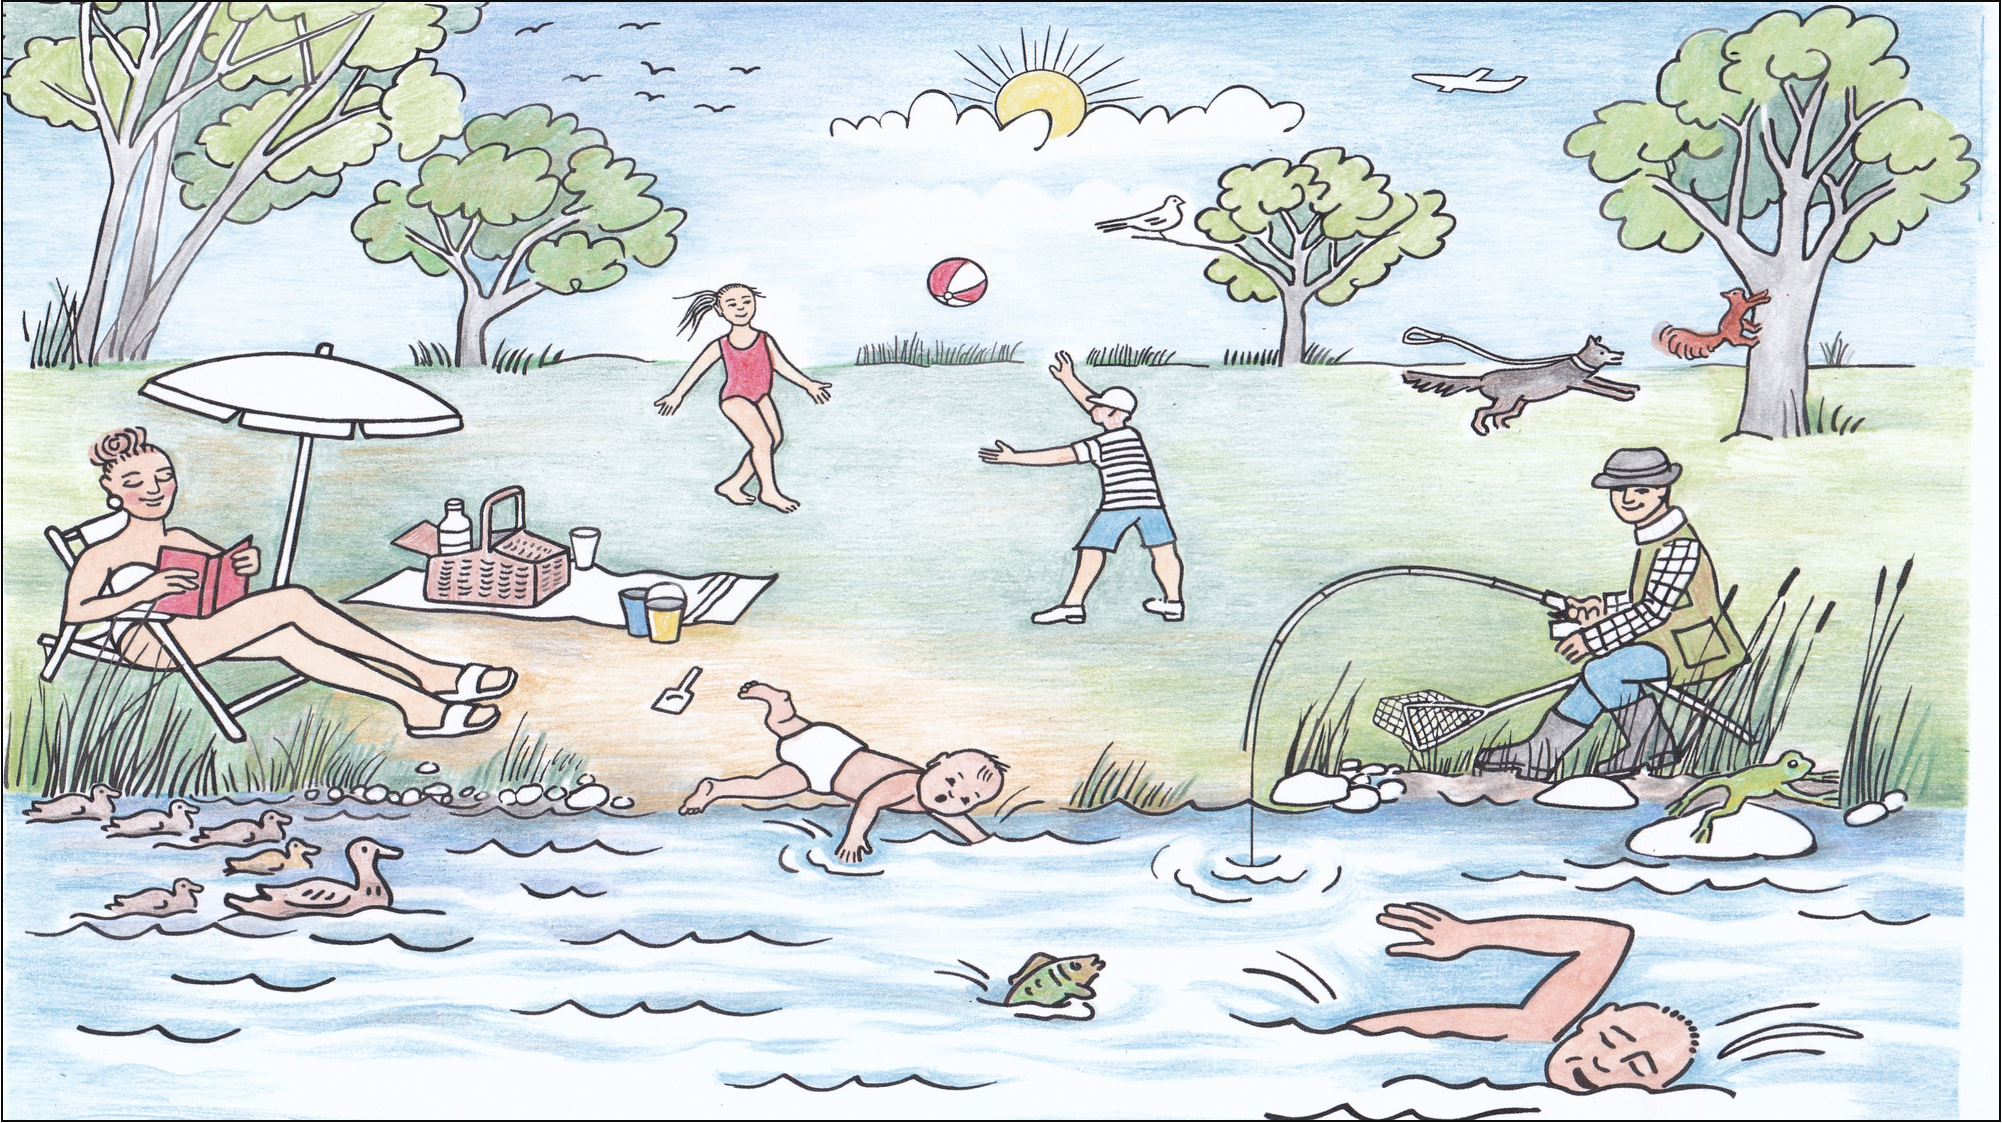
\includegraphics[width=\textwidth]{./src/imgs/summer.png}
	\caption{Kresba použitá pro testování}\label{fig:summer}
\end{figure}

Jak bylo definováno v kapitole~\ref{subsec:reprezentace_znalosti}, referenční popis obrázku se skládá z
množiny objektů, jejich atributů a vazeb mezi nimi.
Nyní bylo potřeba stanovit nějaký datový formát, který by umožnil tuto strukturu dobře zachytit.

\newpage
Základním prvkem referenčního popisu je struktura \enquote{\texttt{Scene}}, která obsahuje informace o obrázku, objekty s atributy a vazby mezi nimi.

Objekty byly definované strukturou \enquote{\texttt{SceneObject}}, která popisuje objekt ve scéně a jeho atributy.
Každý \texttt{SceneObject} obsahuje informaci o svém názvu, umístění, velikosti a hierarchii vůči ostatním objektům.
Dále si každý \texttt{SceneObject} udržuje list atributů a tagů, které mu byly expertem přiděleny.

Další strukturou, která byla definována jako součást referenčního popisu, je \enquote{\texttt{Triplet}}.
Tato struktura slouží k popisu vazeb mezi objekty, obsahuje názvy dvou objektů a k nim název vazby.

Schéma implementovaných struktur a jejich provázání je na Obrázku~\ref{fig:schema_impl_ref_popis}.
Zkratka pro datový typ \texttt{u32} znamená \enquote{unsigned 32-bit int} a je to nezáporné celé číslo na 32 bitech,
druhý typ \texttt{Vec<T>} pak značí vektor (list) objektů typu \texttt{T}.

\begin{figure}[ht!]
	\centering
	\begin{tikzpicture}
		\node[inner sep=0] (ref) at (0, 0) {
			\begin{tabular}{|l|l|l|}
				\hline
				\multicolumn{2}{|c|}{\large \texttt{Scene}}                    \\
				\hline
				\textbf{\textit{Pole}} & \textbf{\textit{Datový typ}}          \\
				\hline
				{width}                & \texttt{u32}                          \\
				{height}               & \texttt{u32}                          \\
				{image\_path}          & \texttt{String}                       \\
				{objects}              & \texttt{Vec<\phantom{ SceneObject }>} \\
				{triplets}             & \texttt{Vec<\phantom{ Triplet }>}     \\
				\hline
			\end{tabular}
		};
		\node[anchor=north, inner sep=1pt] (trip) at ($(ref.south) + (0, -1)$) {
			\begin{tabular}{|l|l|l|}
				\hline
				\multicolumn{2}{|c|}{\large \texttt{Triplet}}         \\
				\hline
				\textbf{\textit{Pole}} & \textbf{\textit{Datový typ}} \\
				\hline
				{from}                 & \texttt{String}              \\
				{predicate}            & \texttt{String}              \\
				{to}                   & \texttt{String}              \\
				\hline
			\end{tabular}
		};
		\node[anchor=north west, inner sep=1pt] (so) at ($(trip.north east) + (1, 0)$) {
			\begin{tabular}{|l|l|l|}
				\hline
				\multicolumn{2}{|c|}{\large \texttt{SceneObject}}       \\
				\hline
				\textbf{\textit{Pole}} & \textbf{\textit{Datový typ}}   \\
				\hline
				{name}                 & \texttt{String}                \\
				{tags}                 & \texttt{Vec<String>}           \\
				{top\_left\_corner}    & \texttt{(u32, u32)}            \\
				{size}                 & \texttt{(u32, u32)}            \\
				{parents}              & \texttt{Vec<String>}           \\
				{children}             & \texttt{Vec<String>}           \\
				{attributes}           & \texttt{Vec<(String, String)>} \\
				\hline
			\end{tabular}
		};
		\node[anchor=south east] (somark) at ($(ref.south east) + (-14.5pt, \baselineskip)$) {\texttt{SceneObject}};
		\node[anchor=south east] (trmark) at ($(ref.south east) + (-39.5pt, 0)$) {\texttt{Triplet}};
		\node[draw=blue, thick,rounded corners=2mm, inner sep=3pt] (trborder) at ($(trmark) + (0, 0.5pt)$) {{\phantom{\texttt{Triplet}}}};
		\node[draw=blue,thick, rounded corners=2mm, inner sep=3pt] (soborder) at ($(somark) + (0, 0.5pt)$) {{\phantom{\texttt{SceneObject}}}};
		\draw[blue,thick, -Stealth] (trborder.south) to (trmark|-trip.north);
		\draw[blue,thick, rounded corners=2mm, -Stealth] (soborder.north) -- ++(0, 0.5) -| (so.north);
		% \draw[blue, rounded corners=3mm, -Stealth] (soborder.north) |- ($(0, 0.2) + (so.west)$);
	\end{tikzpicture}
	\caption{Schéma implementace referenčního popisu}\label{fig:schema_impl_ref_popis}
\end{figure}

Ve struktuře \texttt{Scene} je význam jednotlivých polí poměrně jednoduchý.
Pole \texttt{width} a \texttt{height} vyjadřují výšku a šířku obrázku v pixelech, \texttt{image\_path} udává cestu k souboru, který obsahuje samotný obrázek.
Pole \texttt{objects} a \texttt{triplets} pak obsahují list objektů a tripletů.

Struktura \texttt{Triplet} je velmi jednoduchá.
Její pole \texttt{from} a \texttt{to} jsou názvy zdrojového, respektive cílového, objektu.
Pole \texttt{predicate} je název samotné vazby mezi těmito objekty.

Poslední struktura \texttt{SceneObject}, která popisuje samotné objekty, je nejsložitější.
Pole \texttt{name} udává název daného objektu, který slouží zároveň jako identifikátor a musí být tudíž unikátní.
Může nastat situace, že v obrázku bude více objektů, které by přirozeně byly označené stejně, například dva stromy.
Pro tento případ byla implementována možnost objekty číslovat a tím tak jednoznačně rozlišit i objekty stejného typu.
Číslování objektů je součástí jejich názvu a má formát \enquote{\texttt{\#n}} kde $n$ je přirozené číslo označující index objektu.
Například \enquote{\texttt{strom \#1}} a \enquote{\texttt{strom \#2}}.

Dvojice polí \texttt{top\_left\_corner} a \texttt{size} udávají velikost a pozici objektu zdrojovém obrázku.
Jedná se o souřadnice levého horního rohu ohraničujícího rámce (bounding-boxu) a velikost tohoto rámce v pixelech.
Obě pole mají jako uvedený datový typ \texttt{(u32, u32)}, který reprezentuje souřadnice $(i, j)$ kde $i,j \in \mathbb{N}^{0}$.
V obrázku je jako počátek souřadnic uvažován levý horní roh.

Pole \texttt{tags} reprezentuje list tagů, které expert obrázku přiřadil.
Jejich účel byl popsán v kapitole~\ref{subsec:hodnoceni}.
Další dvojice polí \texttt{parents} a \texttt{children} pak reprezentuje list objektů, které jsou rodiče, respektive potomci, daného objektu.

Po formální definice formátů a datový typů bylo potřeba určit, jakým způsobem bude expert referenční popis tvořit.
Pro tuto práci bylo rozhodnuto, že tvorba referenčního popisu bude spočívat v napsání strukturovaného textového souboru.
Zvolen byl textový formát \texttt{JSON}, který představuje dobrý kompromis mezi čitelností člověkem a strojovou zpracovatelností.

Ukázka části referenčního popisu je na Výpisu~\ref{lst:ref_popis_real_example}.
\clearpage
% \def\lstlabel{label=}
\begin{lstlisting}[
	% there are many more options of styling, see the official documentation, these are just the defaults I like
	frame=single, % make single-line frame around the verbatim
	framesep=2mm, % put some more spacing between the frame and text
	aboveskip=5mm, % put some more space above the box
	basicstyle={\linespread{0.83}\footnotesize\ttfamily}, % use typewriter (monospace) font
	caption={Příklad jednoduchého referenčního popisu}, % set the caption text
	captionpos=b, % put the caption at the bottom (b) or top (t) or both (bt)
	label={lst:ref_popis_real_example}, % label to be referenced via \ref{}
	numbers=left, % line numbers on the left
	numberstyle={\scriptsize\ttfamily\color{black!60}}, % the style for line numbers
	escapeinside={<@}{@>} % between those sequences are command evaluated
]
<@\textcolor[HTML]{FF1010}{\texttt{\{}}@>
<@\textcolor[HTML]{000000}{\texttt{\ \ }}@><@\textcolor[HTML]{255CFF}{\texttt{"width"}}@><@\textcolor[HTML]{1041FF}{\texttt{:}}@><@\textcolor[HTML]{000000}{\texttt{\ }}@><@\textcolor[HTML]{DE6F10}{\texttt{2002}}@><@\textcolor[HTML]{1041FF}{\texttt{,}}@>
<@\textcolor[HTML]{000000}{\texttt{\ \ }}@><@\textcolor[HTML]{255CFF}{\texttt{"height"}}@><@\textcolor[HTML]{1041FF}{\texttt{:}}@><@\textcolor[HTML]{000000}{\texttt{\ }}@><@\textcolor[HTML]{DE6F10}{\texttt{1123}}@><@\textcolor[HTML]{1041FF}{\texttt{,}}@>
<@\textcolor[HTML]{000000}{\texttt{\ \ }}@><@\textcolor[HTML]{255CFF}{\texttt{"image\_path"}}@><@\textcolor[HTML]{1041FF}{\texttt{:}}@><@\textcolor[HTML]{000000}{\texttt{\ }}@><@\textcolor[HTML]{418310}{\texttt{"./data/imgs/summer.png"}}@><@\textcolor[HTML]{1041FF}{\texttt{,}}@>
<@\textcolor[HTML]{000000}{\texttt{\ \ }}@><@\textcolor[HTML]{255CFF}{\texttt{"objects"}}@><@\textcolor[HTML]{1041FF}{\texttt{:}}@><@\textcolor[HTML]{000000}{\texttt{\ }}@><@\textcolor[HTML]{FF1010}{\texttt{[}}@>
<@\textcolor[HTML]{000000}{\texttt{\ \ \ \ }}@><@\textcolor[HTML]{FF1010}{\texttt{\{}}@>
<@\textcolor[HTML]{000000}{\texttt{\ \ \ \ \ \ }}@><@\textcolor[HTML]{255CFF}{\texttt{"name"}}@><@\textcolor[HTML]{1041FF}{\texttt{:}}@><@\textcolor[HTML]{000000}{\texttt{\ }}@><@\textcolor[HTML]{418310}{\texttt{"tree\ \#1"}}@><@\textcolor[HTML]{1041FF}{\texttt{,}}@>
<@\textcolor[HTML]{000000}{\texttt{\ \ \ \ \ \ }}@><@\textcolor[HTML]{255CFF}{\texttt{"tags"}}@><@\textcolor[HTML]{1041FF}{\texttt{:}}@><@\textcolor[HTML]{000000}{\texttt{\ }}@><@\textcolor[HTML]{FF1010}{\texttt{[}}@><@\textcolor[HTML]{418310}{\texttt{"environment"}}@><@\textcolor[HTML]{FF1010}{\texttt{]}}@><@\textcolor[HTML]{1041FF}{\texttt{,}}@>
<@\textcolor[HTML]{000000}{\texttt{\ \ \ \ \ \ }}@><@\textcolor[HTML]{255CFF}{\texttt{"top\_left\_corner"}}@><@\textcolor[HTML]{1041FF}{\texttt{:}}@><@\textcolor[HTML]{000000}{\texttt{\ }}@><@\textcolor[HTML]{FF1010}{\texttt{[}}@><@\textcolor[HTML]{DE6F10}{\texttt{1194}}@><@\textcolor[HTML]{1041FF}{\texttt{,}}@><@\textcolor[HTML]{000000}{\texttt{\ }}@><@\textcolor[HTML]{DE6F10}{\texttt{146}}@><@\textcolor[HTML]{FF1010}{\texttt{]}}@><@\textcolor[HTML]{1041FF}{\texttt{,}}@>
<@\textcolor[HTML]{000000}{\texttt{\ \ \ \ \ \ }}@><@\textcolor[HTML]{255CFF}{\texttt{"size"}}@><@\textcolor[HTML]{1041FF}{\texttt{:}}@><@\textcolor[HTML]{000000}{\texttt{\ }}@><@\textcolor[HTML]{FF1010}{\texttt{[}}@><@\textcolor[HTML]{DE6F10}{\texttt{264}}@><@\textcolor[HTML]{1041FF}{\texttt{,}}@><@\textcolor[HTML]{000000}{\texttt{\ }}@><@\textcolor[HTML]{DE6F10}{\texttt{220}}@><@\textcolor[HTML]{FF1010}{\texttt{]}}@><@\textcolor[HTML]{1041FF}{\texttt{,}}@>
<@\textcolor[HTML]{000000}{\texttt{\ \ \ \ \ \ }}@><@\textcolor[HTML]{255CFF}{\texttt{"parents"}}@><@\textcolor[HTML]{1041FF}{\texttt{:}}@><@\textcolor[HTML]{000000}{\texttt{\ }}@><@\textcolor[HTML]{FF1010}{\texttt{[}}@><@\textcolor[HTML]{FF1010}{\texttt{]}}@><@\textcolor[HTML]{1041FF}{\texttt{,}}@>
<@\textcolor[HTML]{000000}{\texttt{\ \ \ \ \ \ }}@><@\textcolor[HTML]{255CFF}{\texttt{"children"}}@><@\textcolor[HTML]{1041FF}{\texttt{:}}@><@\textcolor[HTML]{000000}{\texttt{\ }}@><@\textcolor[HTML]{FF1010}{\texttt{[}}@><@\textcolor[HTML]{418310}{\texttt{"branch"}}@><@\textcolor[HTML]{FF1010}{\texttt{]}}@><@\textcolor[HTML]{1041FF}{\texttt{,}}@>
<@\textcolor[HTML]{000000}{\texttt{\ \ \ \ \ \ }}@><@\textcolor[HTML]{255CFF}{\texttt{"attributes"}}@><@\textcolor[HTML]{1041FF}{\texttt{:}}@><@\textcolor[HTML]{000000}{\texttt{\ }}@><@\textcolor[HTML]{FF1010}{\texttt{[}}@>
<@\textcolor[HTML]{000000}{\texttt{\ \ \ \ \ \ \ \ }}@><@\textcolor[HTML]{FF1010}{\texttt{[}}@><@\textcolor[HTML]{418310}{\texttt{"color"}}@><@\textcolor[HTML]{1041FF}{\texttt{,}}@><@\textcolor[HTML]{000000}{\texttt{\ }}@><@\textcolor[HTML]{418310}{\texttt{"green"}}@><@\textcolor[HTML]{FF1010}{\texttt{]}}@><@\textcolor[HTML]{1041FF}{\texttt{,}}@>
<@\textcolor[HTML]{000000}{\texttt{\ \ \ \ \ \ \ \ }}@><@\textcolor[HTML]{FF1010}{\texttt{[}}@><@\textcolor[HTML]{418310}{\texttt{"color"}}@><@\textcolor[HTML]{1041FF}{\texttt{,}}@><@\textcolor[HTML]{000000}{\texttt{\ }}@><@\textcolor[HTML]{418310}{\texttt{"brown"}}@><@\textcolor[HTML]{FF1010}{\texttt{]}}@>
<@\textcolor[HTML]{000000}{\texttt{\ \ \ \ \ \ }}@><@\textcolor[HTML]{FF1010}{\texttt{]}}@>
<@\textcolor[HTML]{000000}{\texttt{\ \ \ \ }}@><@\textcolor[HTML]{FF1010}{\texttt{\}}}@><@\textcolor[HTML]{1041FF}{\texttt{,}}@> <@\textcolor[HTML]{FF1010}{\texttt{\{}}@>
<@\textcolor[HTML]{000000}{\texttt{\ \ \ \ \ \ }}@><@\textcolor[HTML]{255CFF}{\texttt{"name"}}@><@\textcolor[HTML]{1041FF}{\texttt{:}}@><@\textcolor[HTML]{000000}{\texttt{\ }}@><@\textcolor[HTML]{418310}{\texttt{"bird"}}@><@\textcolor[HTML]{1041FF}{\texttt{,}}@>
<@\textcolor[HTML]{000000}{\texttt{\ \ \ \ \ \ }}@><@\textcolor[HTML]{255CFF}{\texttt{"tags"}}@><@\textcolor[HTML]{1041FF}{\texttt{:}}@><@\textcolor[HTML]{000000}{\texttt{\ }}@><@\textcolor[HTML]{FF1010}{\texttt{[}}@><@\textcolor[HTML]{418310}{\texttt{"animal"}}@><@\textcolor[HTML]{FF1010}{\texttt{]}}@><@\textcolor[HTML]{1041FF}{\texttt{,}}@>
<@\textcolor[HTML]{000000}{\texttt{\ \ \ \ \ \ }}@><@\textcolor[HTML]{255CFF}{\texttt{"top\_left\_corner"}}@><@\textcolor[HTML]{1041FF}{\texttt{:}}@><@\textcolor[HTML]{000000}{\texttt{\ }}@><@\textcolor[HTML]{FF1010}{\texttt{[}}@><@\textcolor[HTML]{DE6F10}{\texttt{1095}}@><@\textcolor[HTML]{1041FF}{\texttt{,}}@><@\textcolor[HTML]{000000}{\texttt{\ }}@><@\textcolor[HTML]{DE6F10}{\texttt{193}}@><@\textcolor[HTML]{FF1010}{\texttt{]}}@><@\textcolor[HTML]{1041FF}{\texttt{,}}@>
<@\textcolor[HTML]{000000}{\texttt{\ \ \ \ \ \ }}@><@\textcolor[HTML]{255CFF}{\texttt{"size"}}@><@\textcolor[HTML]{1041FF}{\texttt{:}}@><@\textcolor[HTML]{000000}{\texttt{\ }}@><@\textcolor[HTML]{FF1010}{\texttt{[}}@><@\textcolor[HTML]{DE6F10}{\texttt{93}}@><@\textcolor[HTML]{1041FF}{\texttt{,}}@><@\textcolor[HTML]{000000}{\texttt{\ }}@><@\textcolor[HTML]{DE6F10}{\texttt{47}}@><@\textcolor[HTML]{FF1010}{\texttt{]}}@><@\textcolor[HTML]{1041FF}{\texttt{,}}@>
<@\textcolor[HTML]{000000}{\texttt{\ \ \ \ \ \ }}@><@\textcolor[HTML]{255CFF}{\texttt{"parents"}}@><@\textcolor[HTML]{1041FF}{\texttt{:}}@><@\textcolor[HTML]{000000}{\texttt{\ }}@><@\textcolor[HTML]{FF1010}{\texttt{[}}@><@\textcolor[HTML]{FF1010}{\texttt{]}}@><@\textcolor[HTML]{1041FF}{\texttt{,}}@>
<@\textcolor[HTML]{000000}{\texttt{\ \ \ \ \ \ }}@><@\textcolor[HTML]{255CFF}{\texttt{"children"}}@><@\textcolor[HTML]{1041FF}{\texttt{:}}@><@\textcolor[HTML]{000000}{\texttt{\ }}@><@\textcolor[HTML]{FF1010}{\texttt{[}}@><@\textcolor[HTML]{FF1010}{\texttt{]}}@><@\textcolor[HTML]{1041FF}{\texttt{,}}@>
<@\textcolor[HTML]{000000}{\texttt{\ \ \ \ \ \ }}@><@\textcolor[HTML]{255CFF}{\texttt{"attributes"}}@><@\textcolor[HTML]{1041FF}{\texttt{:}}@><@\textcolor[HTML]{000000}{\texttt{\ }}@><@\textcolor[HTML]{FF1010}{\texttt{[}}@><@\textcolor[HTML]{FF1010}{\texttt{[}}@><@\textcolor[HTML]{418310}{\texttt{"color"}}@><@\textcolor[HTML]{1041FF}{\texttt{,}}@><@\textcolor[HTML]{000000}{\texttt{\ }}@><@\textcolor[HTML]{418310}{\texttt{"white"}}@><@\textcolor[HTML]{FF1010}{\texttt{]}}@><@\textcolor[HTML]{FF1010}{\texttt{]}}@>
<@\textcolor[HTML]{000000}{\texttt{\ \ \ \ }}@><@\textcolor[HTML]{FF1010}{\texttt{\}}}@><@\textcolor[HTML]{1041FF}{\texttt{,}}@> <@\textcolor[HTML]{FF1010}{\texttt{\{}}@>
<@\textcolor[HTML]{000000}{\texttt{\ \ \ \ \ \ }}@><@\textcolor[HTML]{255CFF}{\texttt{"name"}}@><@\textcolor[HTML]{1041FF}{\texttt{:}}@><@\textcolor[HTML]{000000}{\texttt{\ }}@><@\textcolor[HTML]{418310}{\texttt{"squirrel"}}@><@\textcolor[HTML]{1041FF}{\texttt{,}}@>
<@\textcolor[HTML]{000000}{\texttt{\ \ \ \ \ \ }}@><@\textcolor[HTML]{255CFF}{\texttt{"tags"}}@><@\textcolor[HTML]{1041FF}{\texttt{:}}@><@\textcolor[HTML]{000000}{\texttt{\ }}@><@\textcolor[HTML]{FF1010}{\texttt{[}}@><@\textcolor[HTML]{418310}{\texttt{"animal"}}@><@\textcolor[HTML]{FF1010}{\texttt{]}}@><@\textcolor[HTML]{1041FF}{\texttt{,}}@>
<@\textcolor[HTML]{000000}{\texttt{\ \ \ \ \ \ }}@><@\textcolor[HTML]{255CFF}{\texttt{"top\_left\_corner"}}@><@\textcolor[HTML]{1041FF}{\texttt{:}}@><@\textcolor[HTML]{000000}{\texttt{\ }}@><@\textcolor[HTML]{FF1010}{\texttt{[}}@><@\textcolor[HTML]{DE6F10}{\texttt{1655}}@><@\textcolor[HTML]{1041FF}{\texttt{,}}@><@\textcolor[HTML]{000000}{\texttt{\ }}@><@\textcolor[HTML]{DE6F10}{\texttt{286}}@><@\textcolor[HTML]{FF1010}{\texttt{]}}@><@\textcolor[HTML]{1041FF}{\texttt{,}}@>
<@\textcolor[HTML]{000000}{\texttt{\ \ \ \ \ \ }}@><@\textcolor[HTML]{255CFF}{\texttt{"size"}}@><@\textcolor[HTML]{1041FF}{\texttt{:}}@><@\textcolor[HTML]{000000}{\texttt{\ }}@><@\textcolor[HTML]{FF1010}{\texttt{[}}@><@\textcolor[HTML]{DE6F10}{\texttt{116}}@><@\textcolor[HTML]{1041FF}{\texttt{,}}@><@\textcolor[HTML]{000000}{\texttt{\ }}@><@\textcolor[HTML]{DE6F10}{\texttt{76}}@><@\textcolor[HTML]{FF1010}{\texttt{]}}@><@\textcolor[HTML]{1041FF}{\texttt{,}}@>
<@\textcolor[HTML]{000000}{\texttt{\ \ \ \ \ \ }}@><@\textcolor[HTML]{255CFF}{\texttt{"parents"}}@><@\textcolor[HTML]{1041FF}{\texttt{:}}@><@\textcolor[HTML]{000000}{\texttt{\ }}@><@\textcolor[HTML]{FF1010}{\texttt{[}}@><@\textcolor[HTML]{FF1010}{\texttt{]}}@><@\textcolor[HTML]{1041FF}{\texttt{,}}@>
<@\textcolor[HTML]{000000}{\texttt{\ \ \ \ \ \ }}@><@\textcolor[HTML]{255CFF}{\texttt{"children"}}@><@\textcolor[HTML]{1041FF}{\texttt{:}}@><@\textcolor[HTML]{000000}{\texttt{\ }}@><@\textcolor[HTML]{FF1010}{\texttt{[}}@><@\textcolor[HTML]{FF1010}{\texttt{]}}@><@\textcolor[HTML]{1041FF}{\texttt{,}}@>
<@\textcolor[HTML]{000000}{\texttt{\ \ \ \ \ \ }}@><@\textcolor[HTML]{255CFF}{\texttt{"attributes"}}@><@\textcolor[HTML]{1041FF}{\texttt{:}}@><@\textcolor[HTML]{000000}{\texttt{\ }}@><@\textcolor[HTML]{FF1010}{\texttt{[}}@>
<@\textcolor[HTML]{000000}{\texttt{\ \ \ \ \ \ \ \ }}@><@\textcolor[HTML]{FF1010}{\texttt{[}}@><@\textcolor[HTML]{418310}{\texttt{"color"}}@><@\textcolor[HTML]{1041FF}{\texttt{,}}@><@\textcolor[HTML]{000000}{\texttt{\ }}@><@\textcolor[HTML]{418310}{\texttt{"orange"}}@><@\textcolor[HTML]{FF1010}{\texttt{]}}@><@\textcolor[HTML]{1041FF}{\texttt{,}}@>
<@\textcolor[HTML]{000000}{\texttt{\ \ \ \ \ \ \ \ }}@><@\textcolor[HTML]{FF1010}{\texttt{[}}@><@\textcolor[HTML]{418310}{\texttt{"color"}}@><@\textcolor[HTML]{1041FF}{\texttt{,}}@><@\textcolor[HTML]{000000}{\texttt{\ }}@><@\textcolor[HTML]{418310}{\texttt{"brown"}}@><@\textcolor[HTML]{FF1010}{\texttt{]}}@>
<@\textcolor[HTML]{000000}{\texttt{\ \ \ \ \ \ }}@><@\textcolor[HTML]{FF1010}{\texttt{]}}@>
<@\textcolor[HTML]{000000}{\texttt{\ \ \ \ }}@><@\textcolor[HTML]{FF1010}{\texttt{\}}}@><@\textcolor[HTML]{1041FF}{\texttt{,}}@> <@\textcolor[HTML]{FF1010}{\texttt{\{}}@>
<@\textcolor[HTML]{000000}{\texttt{\ \ \ \ \ \ }}@><@\textcolor[HTML]{255CFF}{\texttt{"name"}}@><@\textcolor[HTML]{1041FF}{\texttt{:}}@><@\textcolor[HTML]{000000}{\texttt{\ }}@><@\textcolor[HTML]{418310}{\texttt{"bird"}}@><@\textcolor[HTML]{1041FF}{\texttt{,}}@>
<@\textcolor[HTML]{000000}{\texttt{\ \ \ \ \ \ }}@><@\textcolor[HTML]{255CFF}{\texttt{"tags"}}@><@\textcolor[HTML]{1041FF}{\texttt{:}}@><@\textcolor[HTML]{000000}{\texttt{\ }}@><@\textcolor[HTML]{FF1010}{\texttt{[}}@><@\textcolor[HTML]{418310}{\texttt{"animal"}}@><@\textcolor[HTML]{FF1010}{\texttt{]}}@><@\textcolor[HTML]{1041FF}{\texttt{,}}@>
<@\textcolor[HTML]{000000}{\texttt{\ \ \ \ \ \ }}@><@\textcolor[HTML]{255CFF}{\texttt{"top\_left\_corner"}}@><@\textcolor[HTML]{1041FF}{\texttt{:}}@><@\textcolor[HTML]{000000}{\texttt{\ }}@><@\textcolor[HTML]{FF1010}{\texttt{[}}@><@\textcolor[HTML]{DE6F10}{\texttt{1095}}@><@\textcolor[HTML]{1041FF}{\texttt{,}}@><@\textcolor[HTML]{000000}{\texttt{\ }}@><@\textcolor[HTML]{DE6F10}{\texttt{193}}@><@\textcolor[HTML]{FF1010}{\texttt{]}}@><@\textcolor[HTML]{1041FF}{\texttt{,}}@>
<@\textcolor[HTML]{000000}{\texttt{\ \ \ \ \ \ }}@><@\textcolor[HTML]{255CFF}{\texttt{"size"}}@><@\textcolor[HTML]{1041FF}{\texttt{:}}@><@\textcolor[HTML]{000000}{\texttt{\ }}@><@\textcolor[HTML]{FF1010}{\texttt{[}}@><@\textcolor[HTML]{DE6F10}{\texttt{93}}@><@\textcolor[HTML]{1041FF}{\texttt{,}}@><@\textcolor[HTML]{000000}{\texttt{\ }}@><@\textcolor[HTML]{DE6F10}{\texttt{47}}@><@\textcolor[HTML]{FF1010}{\texttt{]}}@><@\textcolor[HTML]{1041FF}{\texttt{,}}@>
<@\textcolor[HTML]{000000}{\texttt{\ \ \ \ \ \ }}@><@\textcolor[HTML]{255CFF}{\texttt{"parents"}}@><@\textcolor[HTML]{1041FF}{\texttt{:}}@><@\textcolor[HTML]{000000}{\texttt{\ }}@><@\textcolor[HTML]{FF1010}{\texttt{[}}@><@\textcolor[HTML]{FF1010}{\texttt{]}}@><@\textcolor[HTML]{1041FF}{\texttt{,}}@>
<@\textcolor[HTML]{000000}{\texttt{\ \ \ \ \ \ }}@><@\textcolor[HTML]{255CFF}{\texttt{"children"}}@><@\textcolor[HTML]{1041FF}{\texttt{:}}@><@\textcolor[HTML]{000000}{\texttt{\ }}@><@\textcolor[HTML]{FF1010}{\texttt{[}}@><@\textcolor[HTML]{FF1010}{\texttt{]}}@><@\textcolor[HTML]{1041FF}{\texttt{,}}@>
<@\textcolor[HTML]{000000}{\texttt{\ \ \ \ \ \ }}@><@\textcolor[HTML]{255CFF}{\texttt{"attributes"}}@><@\textcolor[HTML]{1041FF}{\texttt{:}}@><@\textcolor[HTML]{000000}{\texttt{\ }}@><@\textcolor[HTML]{FF1010}{\texttt{[}}@><@\textcolor[HTML]{FF1010}{\texttt{[}}@><@\textcolor[HTML]{418310}{\texttt{"color"}}@><@\textcolor[HTML]{1041FF}{\texttt{,}}@><@\textcolor[HTML]{000000}{\texttt{\ }}@><@\textcolor[HTML]{418310}{\texttt{"white"}}@><@\textcolor[HTML]{FF1010}{\texttt{]}}@><@\textcolor[HTML]{FF1010}{\texttt{]}}@>
<@\textcolor[HTML]{000000}{\texttt{\ \ \ \ }}@><@\textcolor[HTML]{FF1010}{\texttt{\}}}@><@\textcolor[HTML]{1041FF}{\texttt{,}}@> <@\textcolor[HTML]{FF1010}{\texttt{\{}}@>
<@\textcolor[HTML]{000000}{\texttt{\ \ \ \ \ \ }}@><@\textcolor[HTML]{255CFF}{\texttt{"name"}}@><@\textcolor[HTML]{1041FF}{\texttt{:}}@><@\textcolor[HTML]{000000}{\texttt{\ }}@><@\textcolor[HTML]{418310}{\texttt{"branch"}}@><@\textcolor[HTML]{1041FF}{\texttt{,}}@>
<@\textcolor[HTML]{000000}{\texttt{\ \ \ \ \ \ }}@><@\textcolor[HTML]{255CFF}{\texttt{"tags"}}@><@\textcolor[HTML]{1041FF}{\texttt{:}}@><@\textcolor[HTML]{000000}{\texttt{\ }}@><@\textcolor[HTML]{FF1010}{\texttt{[}}@><@\textcolor[HTML]{418310}{\texttt{"environment"}}@><@\textcolor[HTML]{1041FF}{\texttt{,}}@><@\textcolor[HTML]{000000}{\texttt{\ }}@><@\textcolor[HTML]{418310}{\texttt{"background"}}@><@\textcolor[HTML]{FF1010}{\texttt{]}}@><@\textcolor[HTML]{1041FF}{\texttt{,}}@>
<@\textcolor[HTML]{000000}{\texttt{\ \ \ \ \ \ }}@><@\textcolor[HTML]{255CFF}{\texttt{"top\_left\_corner"}}@><@\textcolor[HTML]{1041FF}{\texttt{:}}@><@\textcolor[HTML]{000000}{\texttt{\ }}@><@\textcolor[HTML]{FF1010}{\texttt{[}}@><@\textcolor[HTML]{DE6F10}{\texttt{1130}}@><@\textcolor[HTML]{1041FF}{\texttt{,}}@><@\textcolor[HTML]{000000}{\texttt{\ }}@><@\textcolor[HTML]{DE6F10}{\texttt{233}}@><@\textcolor[HTML]{FF1010}{\texttt{]}}@><@\textcolor[HTML]{1041FF}{\texttt{,}}@>
<@\textcolor[HTML]{000000}{\texttt{\ \ \ \ \ \ }}@><@\textcolor[HTML]{255CFF}{\texttt{"size"}}@><@\textcolor[HTML]{1041FF}{\texttt{:}}@><@\textcolor[HTML]{000000}{\texttt{\ }}@><@\textcolor[HTML]{FF1010}{\texttt{[}}@><@\textcolor[HTML]{DE6F10}{\texttt{138}}@><@\textcolor[HTML]{1041FF}{\texttt{,}}@><@\textcolor[HTML]{000000}{\texttt{\ }}@><@\textcolor[HTML]{DE6F10}{\texttt{41}}@><@\textcolor[HTML]{FF1010}{\texttt{]}}@><@\textcolor[HTML]{1041FF}{\texttt{,}}@>
<@\textcolor[HTML]{000000}{\texttt{\ \ \ \ \ \ }}@><@\textcolor[HTML]{255CFF}{\texttt{"parents"}}@><@\textcolor[HTML]{1041FF}{\texttt{:}}@><@\textcolor[HTML]{000000}{\texttt{\ }}@><@\textcolor[HTML]{FF1010}{\texttt{[}}@><@\textcolor[HTML]{418310}{\texttt{"tree\ \#1"}}@><@\textcolor[HTML]{FF1010}{\texttt{]}}@><@\textcolor[HTML]{1041FF}{\texttt{,}}@>
<@\textcolor[HTML]{000000}{\texttt{\ \ \ \ \ \ }}@><@\textcolor[HTML]{255CFF}{\texttt{"children"}}@><@\textcolor[HTML]{1041FF}{\texttt{:}}@><@\textcolor[HTML]{000000}{\texttt{\ }}@><@\textcolor[HTML]{FF1010}{\texttt{[}}@><@\textcolor[HTML]{FF1010}{\texttt{]}}@><@\textcolor[HTML]{1041FF}{\texttt{,}}@>
<@\textcolor[HTML]{000000}{\texttt{\ \ \ \ \ \ }}@><@\textcolor[HTML]{255CFF}{\texttt{"attributes"}}@><@\textcolor[HTML]{1041FF}{\texttt{:}}@><@\textcolor[HTML]{000000}{\texttt{\ }}@><@\textcolor[HTML]{FF1010}{\texttt{[}}@><@\textcolor[HTML]{FF1010}{\texttt{]}}@>
<@\textcolor[HTML]{000000}{\texttt{\ \ \ \ }}@><@\textcolor[HTML]{FF1010}{\texttt{\}}}@>
<@\textcolor[HTML]{000000}{\texttt{\ \ }}@><@\textcolor[HTML]{FF1010}{\texttt{]}}@><@\textcolor[HTML]{1041FF}{\texttt{,}}@>
<@\textcolor[HTML]{000000}{\texttt{\ \ }}@><@\textcolor[HTML]{255CFF}{\texttt{"triplets"}}@><@\textcolor[HTML]{1041FF}{\texttt{:}}@><@\textcolor[HTML]{000000}{\texttt{\ }}@><@\textcolor[HTML]{FF1010}{\texttt{[}}@>
<@\textcolor[HTML]{000000}{\texttt{\ \ \ \ }}@><@\textcolor[HTML]{FF1010}{\texttt{\{}}@><@\textcolor[HTML]{255CFF}{\texttt{"from"}}@><@\textcolor[HTML]{1041FF}{\texttt{:}}@><@\textcolor[HTML]{000000}{\texttt{\ }}@><@\textcolor[HTML]{418310}{\texttt{"bird"}}@><@\textcolor[HTML]{1041FF}{\texttt{,}}@><@\textcolor[HTML]{000000}{\texttt{\ }}@><@\textcolor[HTML]{255CFF}{\texttt{"predicate"}}@><@\textcolor[HTML]{1041FF}{\texttt{:}}@><@\textcolor[HTML]{000000}{\texttt{\ }}@><@\textcolor[HTML]{418310}{\texttt{"sitting\ on"}}@><@\textcolor[HTML]{1041FF}{\texttt{,}}@><@\textcolor[HTML]{000000}{\texttt{\ }}@><@\textcolor[HTML]{255CFF}{\texttt{"to"}}@><@\textcolor[HTML]{1041FF}{\texttt{:}}@><@\textcolor[HTML]{000000}{\texttt{\ }}@><@\textcolor[HTML]{418310}{\texttt{"branch"}}@><@\textcolor[HTML]{FF1010}{\texttt{\}}}@><@\textcolor[HTML]{1041FF}{\texttt{,}}@>
<@\textcolor[HTML]{000000}{\texttt{\ \ \ \ }}@><@\textcolor[HTML]{FF1010}{\texttt{\{}}@><@\textcolor[HTML]{255CFF}{\texttt{"from"}}@><@\textcolor[HTML]{1041FF}{\texttt{:}}@><@\textcolor[HTML]{000000}{\texttt{\ }}@><@\textcolor[HTML]{418310}{\texttt{"bird"}}@><@\textcolor[HTML]{1041FF}{\texttt{,}}@><@\textcolor[HTML]{000000}{\texttt{\ }}@><@\textcolor[HTML]{255CFF}{\texttt{"predicate"}}@><@\textcolor[HTML]{1041FF}{\texttt{:}}@><@\textcolor[HTML]{000000}{\texttt{\ }}@><@\textcolor[HTML]{418310}{\texttt{"sitting\ on"}}@><@\textcolor[HTML]{1041FF}{\texttt{,}}@><@\textcolor[HTML]{000000}{\texttt{\ }}@><@\textcolor[HTML]{255CFF}{\texttt{"to"}}@><@\textcolor[HTML]{1041FF}{\texttt{:}}@><@\textcolor[HTML]{000000}{\texttt{\ }}@><@\textcolor[HTML]{418310}{\texttt{"tree\ \#1"}}@><@\textcolor[HTML]{FF1010}{\texttt{\}}}@><@\textcolor[HTML]{1041FF}{\texttt{,}}@>
<@\textcolor[HTML]{000000}{\texttt{\ \ \ \ }}@><@\textcolor[HTML]{FF1010}{\texttt{\{}}@><@\textcolor[HTML]{255CFF}{\texttt{"from"}}@><@\textcolor[HTML]{1041FF}{\texttt{:}}@><@\textcolor[HTML]{000000}{\texttt{\ }}@><@\textcolor[HTML]{418310}{\texttt{"squirrel"}}@><@\textcolor[HTML]{1041FF}{\texttt{,}}@><@\textcolor[HTML]{000000}{\texttt{\ }}@><@\textcolor[HTML]{255CFF}{\texttt{"predicate"}}@><@\textcolor[HTML]{1041FF}{\texttt{:}}@><@\textcolor[HTML]{000000}{\texttt{\ }}@><@\textcolor[HTML]{418310}{\texttt{"climbing"}}@><@\textcolor[HTML]{1041FF}{\texttt{,}}@><@\textcolor[HTML]{000000}{\texttt{\ }}@><@\textcolor[HTML]{255CFF}{\texttt{"to"}}@><@\textcolor[HTML]{1041FF}{\texttt{:}}@><@\textcolor[HTML]{000000}{\texttt{\ }}@><@\textcolor[HTML]{418310}{\texttt{"tree\ \#1"}}@><@\textcolor[HTML]{FF1010}{\texttt{\}}}@><@\textcolor[HTML]{1041FF}{\texttt{,}}@>
<@\textcolor[HTML]{000000}{\texttt{\ \ \ \ }}@><@\textcolor[HTML]{FF1010}{\texttt{\{}}@><@\textcolor[HTML]{255CFF}{\texttt{"from"}}@><@\textcolor[HTML]{1041FF}{\texttt{:}}@><@\textcolor[HTML]{000000}{\texttt{\ }}@><@\textcolor[HTML]{418310}{\texttt{"squirrel"}}@><@\textcolor[HTML]{1041FF}{\texttt{,}}@><@\textcolor[HTML]{000000}{\texttt{\ }}@><@\textcolor[HTML]{255CFF}{\texttt{"predicate"}}@><@\textcolor[HTML]{1041FF}{\texttt{:}}@><@\textcolor[HTML]{000000}{\texttt{\ }}@><@\textcolor[HTML]{418310}{\texttt{"under"}}@><@\textcolor[HTML]{1041FF}{\texttt{,}}@><@\textcolor[HTML]{000000}{\texttt{\ }}@><@\textcolor[HTML]{255CFF}{\texttt{"to"}}@><@\textcolor[HTML]{1041FF}{\texttt{:}}@><@\textcolor[HTML]{000000}{\texttt{\ }}@><@\textcolor[HTML]{418310}{\texttt{"bird"}}@><@\textcolor[HTML]{FF1010}{\texttt{\}}}@>
<@\textcolor[HTML]{000000}{\texttt{\ \ }}@><@\textcolor[HTML]{FF1010}{\texttt{]}}@>
<@\textcolor[HTML]{FF1010}{\texttt{\}}}@>

\end{lstlisting}


\subsubsection{Validace referenčního popisu}
Jak bylo právě ukázáno, tvorba referenčního popisu je ve své podstatě psaní JSON souboru podle nějaké definované struktury a pravidel.
Program při zpracovávání referenčního popisu předpokládá, že data budou validní a odmítne referenční popis, který by obsahoval chyby.
Pro komplexnější scénu však může být náročné pro lidského experta neudělat v popise žádnou chybu a udržet celý referenční popis validní.

Z toho důvodu byl implementován v rámci celého programu příkaz \texttt{check}, který zajišťuje kontrolu všech dříve definovaných pravidel, které musí referenční popis splňovat:
\begin{enumerate}
	\item \textbf{Kontrola názvů objektů}\\
	      Protože je název objektu použit jako identifikátor, tak musí být unikátní a žádné dva objekty ve scéně nesmí mít shodný název.
	      V případě, že by referenční popis obsahoval duplicitní názvy objektů, program na tyto konflikty upozorní.
	\item \textbf{Kontrola přetékání objektů}\\
	      Jelikož má program k dispozici informace o velikosti obrázku (v pixelech) a zároveň pro jednotlivé objekty také jejich pozici a velikost,
	      tak lze předem ověřit, zda uvedené ohraničující rámce nezasahují mimo obrázek.
	      Pokud se tak stane, program vypíše varovné hlášení a upozorní na jednotlivé problematické hodnoty.
	\item \textbf{Kontrola referencí na objekty}\\
	      Objekty mohou v rámci hierarchie odkazovat na jiné objekty.
	      Aby byly tyto reference validní, tak objekt nesmí odkazovat sám na sebe, referovaný objekt musí existovat a hierarchické vazby musí být oboustranné.
	      Tím je myšleno to, že pokud objekt \texttt{\color{red!80!black}A} specifikuje objekt \texttt{\color{red!80!black}B} jako svého rodiče,
	      pak musí i objekt \texttt{\color{red!80!black}B} specifikovat \texttt{\color{red!80!black}A} jako svého potomka a naopak.

	      V případě, že by byly detekované nějaké invalidní odkazy, bude opět vypsáno varovné hlášení o tom, co je v referenčním popise špatně.
	\item \textbf{Kontrola referencí v tripletech}\\
	      Při specifikaci vazeb mezi objekty jsou také odkazované dva objekty.
	      Aby byl triplet validní, musí být oba referované objekty definované ve scéně.
	      V opačném případě bude vypsáno chybové hlášení s informací o chybějících objekty v tripletech.
\end{enumerate}

\subsubsection{Další příkazy pro práci s referenčním popisem}
Kromě příkazu na kontrolu referenčního popisu byly implementované ještě následující pomocné příkazy.
Tyto příkazy slouží obecně k prohlížení a porovnávání referenčních popisů a byly implementované zejména pro situace, kdy by bylo potřeba analyzovat komplexnější scény, porovnávat je mezi sebou a získat obecný přehled o scéně, aniž by potřeba zkoumat samotné JSON soubory.
\begin{enumerate}
	\item \textbf{Příkaz} \texttt{stats}: \\
	      Tento příkaz vypíše základní vybrané statistiky daného referenčního popisu.
	      Hlavním smyslem tohoto příkazu je poskytnout člověku představu o referenčním popisu k němu příslušejícímu obrázku.

	      Příkaz vypíše cestu k souboru s referenčním popisem, dále cestu k souboru,
	      který obsahuje popisovaný obrázek a jeho velikost v pixelech.
	      Dále vypíše počet objektů a počet vazeb (tripletů), které byly v tomto referenčním popise definované.
	\item \textbf{Příkaz} \texttt{list}: \\
	      Příkaz \texttt{list} slouží k vypsání seznamu všech entit daného typu, podobně jako při použití databázových dotazů.
	      Tento příkaz má několik pod-příkazů, které určují, jaký typ informace má být vypsán v podobě seznamu.
	      Může se jednat o objekty, tagy, triplety, atributy, samotné názvy nebo hodnoty atributů,
	      názvy vazeb mezi objekty a další.
	      Seznam všech implementovaných pod-příkazů je možné si prohlédnout ve zdrojovém kódu.

	      Cílem tohoto příkazu je poskytnout rychlý a pohodlný způsob, jak získat seznam všech prvků daného typu ve scéně, aniž by bylo potřeba přímo pracovat se složitější strukturou JSON souboru.
	      Výstup je formátován tak, aby jej bylo možné snadno dále strojově zpracovat a integrovat do komplexnějších sekvencí příkazů.
	\item \textbf{Příkaz} \texttt{crumble}: \\
	      Referenční popis obrazu byl v této práci definován jako množina objektů, jejich atributů a vazeb mezi objekty.
	      Při pohledu na datový typ atributu a tripletu je ale možné si všimnout, že se v podstatě neliší - obojí se skládá ze tří částí,
	      jejichž obsah může být zaměnitelný a rozdíl ve významu je dán pouze zavedenou interpretací.
	      Bylo by tedy možné zobecnit všechny tyto entity a popsat je pouze jedním atomickým datovým typem, který obsahuje dva prvky a vazbu mezi nimi.
	      V této podobě by bylo možné celý referenční popis zobrazit jako tradiční sémantickou síť, kde není rozlišeno, co je vazba mezi objekty a co je pouze popis vlastnosti.

	      Referenční popis nebyl navržen tímto obecnějším způsobem z toho důvodu, že pro komplexnější scény by počet těchto atomických trojic dosahoval tak vysokých hodnot,
	      že by pro lidského experta bylo velmi obtížné se v datech orientovat.
	      Pro strojové zpracování a případné vizualizace by ale mohlo být prospěšné, aby byly všechny typy informací prezentované v jednoduchém formátu.
	      Právě k tomu slouží příkaz \texttt{crumble}, který, jak již název napovídá, daný referenční popis \enquote{rozdrobí} a převede všechny informace do množiny prostých trojic.

	      Schématická ukázka procesu \enquote{rozdrobení} je na Obrázku~\ref{fig:crumble_example}.
	      % malý kluk v modrém tričku chytá červený míč
	      \begin{figure}[ht!]
		      \centering
		      \begin{tikzpicture}
			      \footnotesize
			      \matrix[draw, anchor=west] (boy) at (0, 0) {
				      \node {{\textbf{kluk}}}; \\
				      \node {\texttt{stáří:}}; &
				      \node {\texttt{\textit{mladý}}};                 \\
				      \node {\texttt{výraz:}}; &
				      \node {\texttt{\textit{úsměv}}};                 \\
			      };
			      \matrix[draw, anchor=west] (tshirt) at (1.75, -3) {
				      \node  {{\textbf{tričko}}}; \\
				      \node {\texttt{barva:}}; &
				      \node {\texttt{\textit{zelená}}};                  \\
			      };
			      \matrix[draw, anchor=west] (ball) at (-1.75, -3) {
				      \node  {{\textbf{míč}}}; \\
				      \node {\texttt{barva:}}; &
				      \node {\texttt{\textit{červená}}};                  \\
			      };
			      \draw[-Stealth] (boy) to node[midway, above, sloped] {chytá} (ball);
			      \draw[-Stealth] (boy) to node[midway, above, sloped] {nosí} (tshirt);
			      \matrix[draw, anchor=west] (crumb) at ($0.5*(boy.north) + 0.25*(ball.south) + 0.25*(tshirt.south) + (4, 0)$) {
				      \node {\texttt{kluk - stáří - mladý}}; \\
				      \node {\texttt{kluk - výraz - úsměv}}; \\
				      \node {\texttt{kluk - chytá - míč}}; \\
				      \node {\texttt{kluk - nosí - tričko}}; \\
				      \node {\texttt{míč - barva - červená}}; \\
				      \node {\texttt{tričko - barva - zelená}}; \\
			      };
			      \draw[-Stealth] ($(crumb.west) + (-1.5, 0)$) to node[midway, above] {\texttt{crumble}} ($(crumb.west) + (-0.2, 0)$);
		      \end{tikzpicture}
		      \caption{Ukázka procesu \texttt{crumble} (\enquote{rozdrobení})}\label{fig:crumble_example}
	      \end{figure}

	\item \textbf{Příkaz} \texttt{render}: \\
	      Tento příkaz slouží k vytvoření vizuální reprezentace referenčního popisu.

	      Pro správnou funkci tohoto příkazu je nutné, aby byl na počítači dostupný program Graphviz~\cite{graphviz},
	      jehož DOT-engine je použitý pro vytvoření grafické reprezentace.
	      Výhodou grafické prezentace je přehlednost pro člověka, nicméně pro velmi komplexní scény s mnoha vazbami ani grafická reprezentace nemusí být dostatečná.
	      Je vhodné zmínit, že jedním z problémů takto implementované vizualizace je to, že pro scény s mnoha objekty tvoří Graphviz velmi dlouhé a úzké obrázky,
	      protože sázecí mechanismus skládá jednotlivé uzly pod sebe.

	      Grafická prezentace a metody vizualizace jsou nad rámec zadání této práce, proto bylo rozhodnuto, že pro ilustraci tato implementace dostačuje a případné komplexnější
	      způsoby grafické prezentace jsou ponechány jako možná budoucí rozšíření.
\end{enumerate}


\subsection{Sémantické parsování pomocí gramatik}\label{subsec:moje_gramatiky}
Extrakce sémantické informace byla jednou z hlavních řešených problematik.
Jak již bylo řečeno dříve, byl zvolen přístup založený na parsování textu pomocí sémantických bezkontextových gramatik.

Při prvotních experimentech byla použita již existující implementace tohoto konceptu,
\todo{referovat na SpeechCloud}
používající standard SRGS~\cite{srgs}.

Během těchto prvních pokusů ale bylo zjištěno, že funkcionalita, kterou nabízí existující implementace,
nebude pro potřeby této práce postačovat.
Kvůli tomu byla navržena, implementována a otestována vlastní realizace stejného konceptu
analýzy textu pomocí bezkontextových gramatik, která lépe vyhovovala ostatním zde navrženým,
realizovaným a popsaným postupům a metodám.

Detaily této vlastní implementace a rozdíly oproti existujícím variantám jsou popsány v následujících kapitolách.

\subsubsection{Problémy s existující implementací a SRGS}
Při práci s existující implementací SRGS standardu (SpeechCloud)
\todo{referovat SC správně formálně}
vyvstaly následující problémy:
\begin{enumerate}
	\item \textbf{Speciální pravidlo \texttt{\$GARBAGE}}\\
	      První problém, který bylo potřeba vyřešit, byla absence pravidla \texttt{\$GARBAGE}.
	      Jedná se o speciální pravidlo definované ve standardu SRGS, které má tu vlastnost, že dokáže reprezentovat libovolnou promluvu nebo libovolný token.

	      Lze tak velmi efektivně využít v situacích, kdy je potřeba specifikovat výplňová slova,
	      která dopředu není možné odhadnout a nebo nás při analýze textu nezajímají.

	      Existující implementace však neměla toto speciální pravidlo implementováno.
	      To představovalo problém, protože možnost specifikovat libovolný token je jeden ze základních konceptů,
	      na kterém byl celý navržený koncept sémantické analýzy postaven.
	\item \textbf{Návratová datová struktura}\\
	      Existující implementace nevracela ze svého API celý derivační strom, ale pouze list tagů, které se v derivačním stromu nacházely.
	      To znamená, že byla ztracena hierarchická informace derivačního stromu spolu s informací o konkrétních pravidlech,
	      které byly během zpracování textu použité.

	      Tyto informace nebyly zcela nezbytné pro další postup, avšak jejich absence by
	      vyžadovala výrazně složitější definici parsovacích pravidel v bezkontextových gramatikách a
	      s tím samozřejmě spojený složitější systém na zpracování obdržených výsledků.

	      Dostupnost celých derivačních stromů by tedy byla výhodná ve smyslu zjednodušení dalšího postupu.
	\item \textbf{Řešení nejednoznačných situací}\\
	      Třetí problém vycházel z toho, že SRGS standard umožňuje existenci některých situací,
	      kde není jednoznačně dáno, jak má parsování probíhat,
	      a teoreticky je možné získat z jednoho vstupu více různých derivačních stromů.


	      Existující implementace tyto situace dokázala zpracovat, avšak vrátila pouze jeden výsledek,
	      který byl považovaný za nejlepší podle daného kritéria - v tomto případě podle délky zpracovaného textu.

	      Pro sémantickou analýzu textu potřebnou pro získání testovaného popisu by ale bylo výhodné,
	      kdyby bylo možné toto kritérium změnit, a nebo ještě lépe, získat všechna možná řešení.
\end{enumerate}

Po důkladném zvážení těchto problémů bylo rozhodnuto,
že jako nejlepší způsob řešení bude implementace vlastního parseru.

Během reimplementace vlastního parseru byla jako základní reference využita specifikace SRGS~\cite{srgs},
která přesně popisuje chování, funkčnost i syntax gramatik.

V průběhu reimplementace byly ovšem za účelem zjednodušení vynechány některé části SRGS standardu,
které by pro sémantickou analýzu textu v této práci nebyly nijak užitečné a naopak byly přidány nějaké funkce navíc,
které byly pak využity ve zbytku práce.

Výsledkem tak byl nový formát, označený \enquote{Semantic Parsing Grammar Format} (SPGF).
K němu byly samozřejmě vytvořené i základní softwarové nástroje, které nabízí:
\begin{itemize}
	\item kontrolu syntaxe a případné hlášení o syntaktických chybách,
	\item TreeSitter~\cite{treesitter} modul pro obarvení SPGF kódu v textových editorech,
	\item parser SPGF syntaxe s validací obsahu gramatiky i jednotlivých pravidel,
	\item parser přirozeného textu, který využívá právě SPGF gramatiky.
\end{itemize}

\subsubsection{Semantic Parsing Grammar Format (SPGF)}\label{subsubsec:spgf_def}
Základním a nejvyšším prvkem SPGF je \emph{gramatika}.
Na rozdíl od SRGS definice, SPGF gramatika nevyžaduje žádnou hlavičku a nepodporuje dodatečné prvky,
jako deklaraci jazyka nebo meta-dat.
Gramatika má podobu textového souboru, ve kterém je definována množina parsovacích pravidel.

Každé pravidlo se skládá ze svého názvu, který je uvozený symbolem \enquote{\texttt{\$}}.
Název pravidla slouží jako identifikátor, musí být tedy unikátní v dané gramatice.
Druhou částí pravidla je expanze, která reprezentuje tělo pravidla.
Mezi názvem a expanzí pravidla je znak rovnítka \enquote{=}.
Pravidlo je vždy zakončeno středníkem.
Například:
\begin{center}
	\begin{tikzpicture}
		\node[inner sep=0] (dolar) at (0, 0) {\texttt{\strut\$}};
		\node[inner sep=0,anchor=west] (name) at (dolar.east) {\texttt{\strut climbing}};
		\node[inner sep=0,anchor=west] (eq) at (name.east) {\texttt{\strut\phantom{a}=\phantom{a}}};
		\node[inner sep=0,anchor=west] (body) at (eq.east) {\texttt{\strut (leze | šplhá) [na | po]}};
		\node[inner sep=0,anchor=west] (sc) at (body.east) {\texttt{\strut;}};

		\def\downdist{0.0}
		\draw[thick, decorate, decoration={calligraphic brace, mirror, amplitude=4}]
		($(name.south west) + (0, \downdist)$) -- ($(name.south east) + (0, \downdist)$)
		node[pos=0.5, below=3pt] {\scriptsize název pravidla};
		\draw[thick, decorate, decoration={calligraphic brace, mirror, amplitude=4}]
		($(body.south west) + (0, \downdist)$) -- ($(body.south east) + (0, \downdist)$)
		node[pos=0.5, below=3pt] {\scriptsize expanze (tělo pravidla)};
	\end{tikzpicture}
\end{center}

Tělo pravidla se skládá z takzvaných \emph{alternativ}, které jsou oddělené znakem \enquote{\texttt{|}}.
Tato \emph{alternativa} je pak dále definována jako posloupnost \emph{elementů}.
V zápise má přednost mezera před \enquote{\texttt{|}}, takže několik tokenů po sobě je bráno jako jeden celek.
Element má tři varianty, může jím být \emph{token, reference} nebo \emph{sekvence}.
Například:

\begin{center}
	\begin{tikzpicture}
		\node[inner sep=0] (name) at (0, 0) {\texttt{\strut\$dog =\phantom{a}}};
		\node[inner sep=0,anchor=west] (pejsek) at (name.east) {\texttt{\strut pejsek}};
		\node[inner sep=0,anchor=west] (s) at (pejsek.east) {\texttt{\strut\phantom{a}}};
		\node[inner sep=0,anchor=west] (p) at (s.east) {\texttt{\strut |}};
		\node[inner sep=0,anchor=west] (s) at (p.east) {\texttt{\strut\phantom{a}}};
		\node[inner sep=0,anchor=west] (b1) at (s.east) {\texttt{\strut (}};
		\node[inner sep=0,anchor=west] (pes) at (b1.east) {\texttt{\strut pes}};
		\node[inner sep=0,anchor=west] (s) at (pes.east) {\texttt{\strut\phantom{a}}};
		\node[inner sep=0,anchor=west] (p) at (s.east) {\texttt{\strut |}};
		\node[inner sep=0,anchor=west] (s) at (p.east) {\texttt{\strut\phantom{a}}};
		\node[inner sep=0,anchor=west] (psík) at (s.east) {\texttt{\strut psík}};
		\node[inner sep=0,anchor=west] (b2) at (psík.east) {\texttt{\strut )}};
		\node[inner sep=0,anchor=west] (s) at (b2.east) {\texttt{\strut\phantom{a}}};
		\node[inner sep=0,anchor=west] (p) at (s.east) {\texttt{\strut |}};
		\node[inner sep=0,anchor=west] (s) at (p.east) {\texttt{\strut\phantom{a}}};
		\node[inner sep=0,anchor=west] (nej) at (s.east) {\texttt{\strut nejlepší}};
		\node[inner sep=0,anchor=west] (s) at (nej.east) {\texttt{\strut\phantom{a}}};
		\node[inner sep=0,anchor=west] (friend) at (s.east) {\texttt{\strut přítel}};
		\node[inner sep=0,anchor=west] (s) at (friend.east) {\texttt{\strut\phantom{a}}};
		\node[inner sep=0,anchor=west] (human) at (s.east) {\texttt{\strut člověka}};
		\node[inner sep=0,anchor=west] (semicolon) at (human.east) {\texttt{\strut ;}};

		\def\downdist{0.0}
		\draw[thick, decorate, decoration={calligraphic brace, mirror, amplitude=4}]
		($(pejsek.south west) + (0, \downdist)$) -- ($(pejsek.south east) + (0, \downdist)$)
		node[pos=0.5, above=-16pt] {\scriptsize alternativa 1};
		\draw[thick, decorate, decoration={calligraphic brace, mirror, amplitude=4}]
		($(b1.south west) + (0, \downdist)$) -- ($(b2.south east) + (0, \downdist)$)
		node[pos=0.5, above=-16pt] {\scriptsize alternativa 2};
		\draw[thick, decorate, decoration={calligraphic brace, mirror, amplitude=4}]
		($(nej.south west) + (0, \downdist)$) -- ($(human.south east) + (0, \downdist)$)
		node[pos=0.5, above=-16pt] {\scriptsize alternativa 3};

		\def\updist{0.1}

		\draw[thick, decorate, decoration={calligraphic brace, amplitude=4}]
		($(pejsek.north west) + (0, -\updist)$) -- ($(pejsek.north east) + (0, -\updist)$)
		node[pos=0.5, above=3pt] {\scriptsize token};

		% \draw[thick, decorate, decoration={calligraphic brace, amplitude=4}]
		% ($(pes.north west) + (0, -\updist)$) -- ($(pes.north east) + (0, -\updist)$)
		% node[pos=0.5, above=3pt] {\scriptsize token};

		% \draw[thick, decorate, decoration={calligraphic brace, amplitude=4}]
		% ($(psík.north west) + (0, -\updist)$) -- ($(psík.north east) + (0, -\updist)$)
		% node[pos=0.5, above=3pt] {\scriptsize token};

		\draw[thick, decorate, decoration={calligraphic brace, amplitude=4}]
		($(nej.north west) + (0, -\updist)$) -- ($(nej.north east) + (0, -\updist)$)
		node[pos=0.5, above=3pt] {\scriptsize token};

		\draw[thick, decorate, decoration={calligraphic brace, amplitude=4}]
		($(friend.north west) + (0, -\updist)$) -- ($(friend.north east) + (0, -\updist)$)
		node[pos=0.5, above=3pt] {\scriptsize token};

		\draw[thick, decorate, decoration={calligraphic brace, amplitude=4}]
		($(human.north west) + (0, -\updist)$) -- ($(human.north east) + (0, -\updist)$)
		node[pos=0.5, above=3pt] {\scriptsize token};

		\draw[thick, decorate, decoration={calligraphic brace, amplitude=4}]
		($(b1.north west) + (0, -\updist)$) -- ($(b2.north east) + (0, -\updist)$)
		node[pos=0.5, above=3pt] {\scriptsize sekvence};
	\end{tikzpicture}
\end{center}

Nejjednodušší variantou \emph{elementu} je \emph{token}.
Jedná se o terminální symbol (literál), který udává, jaký řetězec je při parsování právě přípustný.
Token je možné chápat jako konkrétní slovo, které je v dané pozici v textu očekávané.
Může se skládat z jednoho nebo více znaků, která mohou být písmena, číslice, tečka, pomlčka, podtržítko nebo dvojtečka.
Součástí definice tokenu může také být (volitelně) definice opakování a případně libovolný počet tagů.
Opakování elementů a tagy budou detailněji popsány později.

Druhou variantou elementu je \emph{reference}.
Tímto pojmem se rozumí odkaz na jiné pravidlo, a nebo odkaz na nějaké speciální pravidlo s vyhrazeným názvem.
Reference začíná symbolem \enquote{\texttt{\$}} po kterém následuje okamžitě (bez mezery) jméno referovaného
pravidla definovaného ve stejné gramatice, nebo speciálního pravidla.
SPGF umožňuje referovat pravidla rekurzivně, a to jak přímo (pravidlo obsahuje referenci na samo sebe), tak v cyklu.

Například jednoduchá gramatika pro (fiktivní) zápis vybraných matematických operací obsahuje rekurzivní pravidlo \texttt{\$expr}:
\begin{verbatim}
	public $expr = $numer | $expr $operator $expr;
	public $number = $digit<+>;
	public $digit = 0 | 1 | 2 | 3 | 4 | 5 | 6 | 7 | 8 | 9 | 10;
	public $operator = plus | minus | dot | frac ;
\end{verbatim}

Formát SPGF definuje 5 speciálních pravidel s vyhraněnými jmény.
Tři z nich jsou převzaté ze SRGS standardu, zbylé dvě byly přidány navíc, aby bylo možné vynutit jistá chování parsovacího algoritmu,
která jsou v SRGS automaticky, ale v SPGF nikoli, kvůli odlišné strategii prohledávání (viz později).
\begin{enumerate}
	\item \textbf{Speciální pravidlo} \texttt{\$GARBAGE}:\\
	      Akceptuje libovolný jeden token a posune parsování o akceptovaný token dále.

	      Speciální pravidlo \texttt{\$GARBAGE} je užitečné, když je potřeba vyjádřit, že na dané pozici v textu
	      může být libovolné slovo, které buďto nedokážeme předvídat, nebo nás nezajímá.
	\item \textbf{Speciální pravidlo} \texttt{\$NULL}:\\
	      Akceptuje prázdný řetězec.
	      To znamená, že je vždy úspěšně aktivováno a nikdy neposune parsování o žádný znak dále.

	      Lze využít například pro situace, kde je žádoucí přidat do derivačního stromu (angl.~parsing tree) nějaké tagy,
	      aniž by byl učiněn postup v parsovaném textu.
	\item \textbf{Speciální pravidlo} \texttt{\$VOID}:\\
	      Vždy selže, bez ohledu na parsovaný text.
	      Nikdy tedy není úspěšné a sekvence obsahující \texttt{\$VOID} také nikdy nebude úspěšná.

	      Lze využít například pro dočasné blokování některých jiných pravidel, nebo pro zdůraznění,
	      že daná sekvence tokenů se nesmí v textu vyskytovat.
	\item \textbf{Speciální pravidlo} \texttt{\$END}:\\
	      Akceptuje konec textu.
	      Bude úspěšné právě ve chvíli, kdy je parsování na konci textu a nezbývá již žádný znak ke zpracování.

	      Umístění speciálního pravidla \texttt{\$END} na konec nějaké expanze tak způsobí,
	      že celá expanze bude úspěšná pouze ve chvíli, kdy dokáže pojmout text beze zbytku až do konce.
	\item \textbf{Speciální pravidlo} \texttt{\$BEGIN}: \\
	      Akceptuje začátek textu.
	      Bude úspěšné právě ve chvíli, kdy je parsování na začátku textu a žádný znak ještě nebyl zpracován.

	      Umístění speciálního pravidla \texttt{\$BEGIN} na začátek expanze tak způsobí,
	      že celá expanze bude úspěšná pouze ve chvíli, kdy dokáže pojmout text od prvního znaku.
\end{enumerate}

Poslední podobu, kterou \emph{element} může mít, je \emph{sekvence}.
Sekvence může být \enquote{obyčejná} nebo \enquote{volitelná}.
V~obou případech se jedná o \emph{alternativy} oddělené znakem \enquote{\texttt{|}},
list alternativ je ohraničený kulatými, respektive hranatými, závorkami.

Důvodem pro existenci \emph{sekvencí} je to, že umožňují seskupování elementů a přehlednější tvorbu složitějších konstrukcí,
podobně jako jsou v matematice používané závorky v aritmetických či algebraických výrazech.
Volitelná sekvence (s hranatými závorkami) je pouze syntaktická zkratka pro \enquote{obyčejnou} sekvenci,
která má minimální počet opakování roven nule (takže se nemusí vůbec v textu vyskytovat) a
maximální počet opakování roven jedné.
Jedná se o obdobu operátoru \enquote{\texttt{?}} v regulárních výrazech.

Příklad zápisu pravidla s oběma typy sekvencí a jeho schématická reprezentace
je pak na Obrázku~\ref{fig:climbing_rule_scheme}.
\begin{figure}[H]
	\centering
	\begin{tikzpicture}
		\node[inner sep=0] (dolar) at (0, 0) {\texttt{\strut\$}};
		\node[inner sep=0,anchor=west] (name) at (dolar.east) {\texttt{\strut climbing}};
		\node[inner sep=0,anchor=west] (eq) at (name.east) {\texttt{\strut\phantom{a}=\phantom{a}}};
		\node[inner sep=0,anchor=west] (b1) at (eq.east) {\texttt{\strut (}};
		\node[inner sep=0,anchor=west] (s) at (b1.east) {\texttt{\strut\phantom{a}}};
		\node[inner sep=0,anchor=west] (leze) at (s.east) {\texttt{\strut leze}};
		\node[inner sep=0,anchor=west] (s) at (leze.east) {\texttt{\strut\phantom{a}}};
		\node[inner sep=0,anchor=west] (p) at (s.east) {\texttt{\strut |}};
		\node[inner sep=0,anchor=west] (s) at (p.east) {\texttt{\strut\phantom{a}}};
		\node[inner sep=0,anchor=west] (šplhá) at (s.east) {\texttt{\strut šplhá}};
		\node[inner sep=0,anchor=west] (s) at (šplhá.east) {\texttt{\strut\phantom{a}}};
		\node[inner sep=0,anchor=west] (b2) at (s.east) {\texttt{\strut )}};
		\node[inner sep=0,anchor=west] (s) at (b2.east) {\texttt{\strut\phantom{a}}};
		\node[inner sep=0,anchor=west] (b3) at (s.east) {\texttt{\strut [}};
		\node[inner sep=0,anchor=west] (s) at (b3.east) {\texttt{\strut\phantom{a}}};
		\node[inner sep=0,anchor=west] (na) at (s.east) {\texttt{\strut na}};
		\node[inner sep=0,anchor=west] (s) at (na.east) {\texttt{\strut\phantom{a}}};
		\node[inner sep=0,anchor=west] (p) at (s.east) {\texttt{\strut |}};
		\node[inner sep=0,anchor=west] (s) at (p.east) {\texttt{\strut\phantom{a}}};
		\node[inner sep=0,anchor=west] (po) at (s.east) {\texttt{\strut po}};
		\node[inner sep=0,anchor=west] (s) at (po.east) {\texttt{\strut\phantom{a}}};
		\node[inner sep=0,anchor=west] (b4) at (s.east) {\texttt{\strut ]}};
		\node[inner sep=0,anchor=west] (sem) at (b4.east) {\texttt{\strut;}};

		\def\downdist{0.0}
		\draw[thick, decorate, decoration={calligraphic brace, mirror, amplitude=4}]
		($(b1.south west) + (0, \downdist)$) -- ($(b2.south east) + (0, \downdist)$)
		node[pos=0.5, below=3pt] {\scriptsize sekvence};

		\draw[thick, decorate, decoration={calligraphic brace, mirror, amplitude=4}]
		($(b3.south west) + (0, \downdist)$) -- ($(b4.south east) + (0, \downdist)$)
		node[pos=0.5, below=3pt] {\scriptsize volitelná sekvence};

		\def\downdist{-0.1}
		\draw[thick, decorate, decoration={calligraphic brace, amplitude=4}]
		($(leze.north west) + (0, \downdist)$) -- ($(šplhá.north east) + (0, \downdist)$)
		node[pos=0.5, above=3pt] {\scriptsize 2 alternativy};
		\draw[thick, decorate, decoration={calligraphic brace, amplitude=4}]
		($(na.north west) + (0, \downdist)$) -- ($(po.north east) + (0, \downdist)$)
		node[pos=0.5, above=3pt] {\scriptsize 2 alternativy};
	\end{tikzpicture}

	\phantom{a} % spacing between the pictures

	\begin{tikzpicture}[inner sep=0pt,rounded corners=2mm]
		\node[draw, minimum width=17mm] (leze) at (0, 0.6) {\texttt{\strut leze}};
		\node[draw, minimum width=17mm] (šplhá) at (0, -0.6)  {\texttt{\strut šplhá}};
		\node[circle,fill,minimum width=5pt] (begin) at ($(leze.west) + (-1, -0.6)$) {};
		\node[draw, minimum width=10mm] (na) at ($(leze) + (3, 0.0)$)  {\texttt{\strut na}};
		\node[draw, minimum width=10mm] (po) at ($(šplhá) + (3, -0.0)$)  {\texttt{\strut po}};
		\node[circle,fill,minimum width=5pt] (end) at ($(na.east) + (1.2, -0.6)$) {};

		\draw[-Stealth] (begin.center) -- ++(0.5, 0) -- ++(0, 0.6) -- (leze.west);
		\draw[-Stealth] (begin.center) -- ++(0.5, 0) -- ++(0, -0.6) -- (šplhá.west);
		\draw[-Stealth] (šplhá.east) -- ++(0.5, 0) -- ++(0, 0.6) -- ($(po.west) + (-0.5, 0.6)$) |- (po.west);
		\draw[-Stealth] (leze.east) -- ++(0.5, 0) -- ++(0, -0.6) -- ($(na.west) + (-0.5, -0.6)$) |- (na.west);
		\draw[-Stealth] ($(na.west) + (-0.7, -0.6)$) -- (end);
		\draw[-Stealth] (na.east) -| ($(na.east) + (0.5, -0.6)$) -- (end);
		\draw[-Stealth] (po.east) -| ($(po.east) + (0.5, 0.6)$) -- (end);
	\end{tikzpicture}
	\caption{Pravidlo \texttt{\$climbing} ve formátu SPGF a v podobě konečného automatu}\label{fig:climbing_rule_scheme}
\end{figure}

\subsubsection{Vstupní a výstupní body SPGF gramatiky}
Základní rozdíl v parsovací strategii SPGF oproti SRGS spočívá v tom, co je považováno za úspěšný konec parsování.
SRGS implementace jako úspěšně dokončené parsování považuje takové situace, kde poskytnutý text byl
pokryt daným pravidlem, obojí (pravidlo i text) vyčerpané (využité) beze zbytku od začátku do konce.
Naproti tomu SPGF parser nekontroluje využití celého textu, pouze celého pravidla.
Pokud tedy pravidlo pokryje pouze prvních několik slov a zbytek textu nebude \enquote{pasovat},
SRGS bude tuto situaci brát jako za neúspěch, zatímco SPGF to bude považovat za úspěch.

Dalším rozdílem mezi SRGS a SPGF je ten, že SRGS gramatiky poskytují pouze jeden vstupní bod (pravidlo označené klíčovým slovem \texttt{root}).
SPGF oproti tomu umožňuje specifikovat více pravidel jako \enquote{veřejná} klíčovým slovem \texttt{public} a tím tak gramatika bude mít více vstupních bodů.
Parser po načtení SPGF gramatiky vezme všechna pravidla označená jako \texttt{public} a pokusí se pomocí nich zpracovat poskytnutý text.
Výsledky úspěšných parsování jsou pak vrácené jako výstupy v podobě derivačních stromů, se kterými je možné dále pracovat.

Pro příklad uvažujme vstupní text: \enquote{\emph{hnědý pes utíká pryč}} a gramatiku na Výpisu~\ref{lst:simple_grammar_1}.
\begin{lstlisting}[
	% there are many more options of styling, see the official documentation, these are just the defaults I like
	frame=single, % make single-line frame around the verbatim
	framesep=2mm, % put some more spacing between the frame and text
	aboveskip=5mm, % put some more space above the box
	basicstyle={\linespread{1.0}\small\ttfamily}, % use typewriter (monospace) font
	caption={Ukázková SPGF gramatika}, % set the caption text
	captionpos=b, % put the caption at the bottom (b) or top (t) or both (bt)
	label={lst:simple_grammar_1}, % label to be referenced via \ref{}
	numbers=left, % line numbers on the left
	numberstyle={\scriptsize\ttfamily\color{black!60}}, % the style for line numbers
	escapeinside={<@}{@>} % between those sequences are command evaluated
]
<@\textcolor[HTML]{8839EF}{\texttt{public}}@><@\textcolor[HTML]{000000}{\texttt{\ }}@><@\textcolor[HTML]{255CFF}{\texttt{\$sentence\ =}}@><@\textcolor[HTML]{000000}{\texttt{\ }}@><@\textcolor[HTML]{724BFF}{\texttt{\$color}}@><@\textcolor[HTML]{000000}{\texttt{\ }}@><@\textcolor[HTML]{724BFF}{\texttt{\$object}}@><@\textcolor[HTML]{000000}{\texttt{\ }}@><@\textcolor[HTML]{724BFF}{\texttt{\$action}}@><@\textcolor[HTML]{1041FF}{\textbf{\texttt{;}}}@>
<@\textcolor[HTML]{255CFF}{\texttt{\$color\ =}}@><@\textcolor[HTML]{000000}{\texttt{\ modrý\ }}@><@\textcolor[HTML]{1041FF}{\textbf{\texttt{|}}}@><@\textcolor[HTML]{000000}{\texttt{\ zelený\ }}@><@\textcolor[HTML]{1041FF}{\textbf{\texttt{|}}}@><@\textcolor[HTML]{000000}{\texttt{\ hnědý}}@><@\textcolor[HTML]{1041FF}{\textbf{\texttt{;}}}@>
<@\textcolor[HTML]{255CFF}{\texttt{\$object\ =}}@><@\textcolor[HTML]{000000}{\texttt{\ pes\ }}@><@\textcolor[HTML]{1041FF}{\textbf{\texttt{|}}}@><@\textcolor[HTML]{000000}{\texttt{\ míč\ }}@><@\textcolor[HTML]{1041FF}{\textbf{\texttt{|}}}@><@\textcolor[HTML]{000000}{\texttt{\ autobus}}@><@\textcolor[HTML]{1041FF}{\textbf{\texttt{;}}}@>
<@\textcolor[HTML]{255CFF}{\texttt{\$action\ =}}@><@\textcolor[HTML]{000000}{\texttt{\ utíká\ }}@><@\textcolor[HTML]{1041FF}{\textbf{\texttt{|}}}@><@\textcolor[HTML]{000000}{\texttt{\ jede\ }}@><@\textcolor[HTML]{1041FF}{\textbf{\texttt{|}}}@><@\textcolor[HTML]{000000}{\texttt{\ [se]\ kutálí}}@><@\textcolor[HTML]{1041FF}{\textbf{\texttt{;}}}@>

\end{lstlisting}


Tuto gramatiku z Výpisu~\ref{lst:simple_grammar_1} lze zakreslit jako konečný automat
na Obrázku~\ref{fig:scheme_grammar_final_automata}.
\begin{figure}[H]
	\centering
	\begin{tikzpicture}[inner sep=0pt, rounded corners=2mm]
		\node[draw, minimum width=17mm] (modrý) at (0, 1)  {\texttt{\strut modrý}};
		\node[draw, minimum width=17mm] (zelený) at (0, 0) {\texttt{\strut zelený}};
		\node[draw, minimum width=17mm] (hnědý) at (0, -1) {\texttt{\strut hnědý}};
		\node[fill, circle, minimum width=5pt] (start) at ($(zelený.west) + (-1, 0)$) {};

		\node[draw, minimum width=20mm, anchor=west] (pes) at ($(modrý.east) + (1.5, 0)$)  {\texttt{\strut pes}};
		\node[draw, minimum width=20mm, anchor=west] (míč) at ($(zelený.east) + (1.5, 0)$) {\texttt{\strut míč}};
		\node[draw, minimum width=20mm, anchor=west] (autobus) at ($(hnědý.east) + (1.5, 0)$) {\texttt{\strut autobus}};

		\node[draw, minimum width=20mm, anchor=west] (utíká) at ($(pes.east) + (3.5, 0)$)  {\texttt{\strut utíká}};
		\node[draw, minimum width=20mm, anchor=west] (jede) at ($(míč.east) + (3.5, 0)$) {\texttt{\strut jede}};
		\node[draw, minimum width=20mm, anchor=west] (kutálí) at ($(autobus.east) + (3.5, 0)$) {\texttt{\strut kutálí}};

		\node[draw, minimum width=10mm, anchor=east] (se) at ($(kutálí.west) + (-1, 0)$) {\texttt{\strut se}};

		\node[fill, circle, minimum width=5pt] (end) at ($(jede.east) + (1.1, 0)$) {};

		\draw[-Stealth] (start.center) -- ($(zelený.west) + (-0.5, 0)$) -- ($(modrý.west) + (-0.5, 0)$) -- (modrý.west);
		\draw[-Stealth] (start.center) -- ($(zelený.west) + (-0.5, 0)$) -- ($(hnědý.west) + (-0.5, 0)$) -- (hnědý.west);
		\draw[-Stealth] (start.center) -- (zelený.west);

		\draw[-Stealth] (modrý.east)
		-- ($(modrý.east) + (0.5, 0)$)
		-- ($(zelený.east) + (0.5, 0)$)
		-- ($(míč.west) + (-0.5, 0)$)
		-- ($(pes.west) + (-0.5, 0)$)
		-- (pes.west);
		\draw[-Stealth] (hnědý.east)
		-- ($(hnědý.east) + (0.5, 0)$)
		-- ($(zelený.east) + (0.5, 0)$)
		-- ($(míč.west) + (-0.5, 0)$)
		-- ($(autobus.west) + (-0.5, 0)$)
		-- (autobus.west);
		\draw[-Stealth] (zelený.east) -- (míč.west);

		\draw[-Stealth] (pes.east)
		-- ++(0.5, 0)
		-- ++(0, -1)
		-- ($(jede.west) + (-0.5, 0)$)
		-- ++(0, 1)
		-- (utíká.west);
		\draw[-Stealth] (autobus.east)
		-- ++(0.5, 0)
		-- ++(0, 1)
		-- ($(jede.west) + (-0.5, 0)$)
		-- ++(0, -1)
		-- (kutálí.west);
		\draw[-Stealth] (míč.east) -- (jede.west);
		\draw[-Stealth] ($(se.west) + (-1, 1)$)
		-- ($(se.west) + (-0.5, 1)$)
		-- ($(se.west) + (-0.5, 0)$)
		-- (se.west);
		\draw[-Stealth] (se.east) -- (kutálí.west);

		\draw[-Stealth] (jede.east) -- (end);
		\draw[-Stealth] (utíká.east) -- ++(0.5, 0) -- ++(0, -1) -- (end);
		\draw[-Stealth] (kutálí.east) -- ++(0.5, 0) -- ++(0, 1) -- (end);
	\end{tikzpicture}
	\caption{Schéma gramatiky jako konečného automatu}\label{fig:scheme_grammar_final_automata}
\end{figure}

Při zpracování textu by mohl vzniknout následující derivační strom, který je na Obrázku~\ref{fig:parsing_tree_example}:
\begin{figure}[H]
	\centering
	\begin{tikzpicture}[anchor=west,inner sep=2pt]
		\def\spacing{40pt}
		\node (w1) at (0,0) {\strut\emph{hnědý}};
		\node (w2) at ($(w1.east) + (\spacing, 0)$) {\strut\emph{pes}};
		\node (w3) at ($(w2.east) + (\spacing, 0)$) {\strut\emph{utíká}};
		\node (w4) at ($(w3.east) + (\spacing, 0)$) {\strut\emph{pryč}};
		\node[anchor=center] (n1) at ($(w1.center) + (0, \spacing)$) {\texttt{\strut\$color}};
		\node[anchor=center] (n2) at ($(w2.center) + (0, \spacing)$) {\texttt{\strut\$object}};
		\node[anchor=center] (n3) at ($(w3.center) + (0, \spacing)$) {\texttt{\strut\$action}};
		\node[anchor=center] (n4) at ($0.5*(n1.west) + 0.5*(n3.east) + (0, \spacing)$) {\texttt{\strut\$sentence}};
		\draw[->] (w1) to (n1);
		\draw[->] (w2) to (n2);
		\draw[->] (w3) to (n3);
		\draw[->] (n1) to (n4);
		\draw[->] (n2) to (n4);
		\draw[->] (n3) to (n4);
	\end{tikzpicture}
	\caption{Ukázkový derivační strom}\label{fig:parsing_tree_example}
\end{figure}

Jak je vidět, poslední slovo \enquote{\emph{pryč}} není součástí derivačního stromu,
protože parsovací pravidlo \texttt{\$sentence} jej nedokáže pokrýt.
V případě SRGS by tento derivační strom byl považovaný za neúspěch, zatímco SPGF vrátí zobrazený parsovací strom
jako úspěšný výsledek.

\subsubsection{Tagy v SPGF}
K elementům je možné přiřadit \emph{tagy}.
Každý tag je libovolný text ohraničený složenými závorkami \enquote{\texttt{\{\}}}.
Za každý element (s výjimkou speciálního pravidla \texttt{\$VOID}) je možné připsat libovolný počet těchto tagů,
oddělených mezerami.

Tagy v SPGF nijak neovlivňují parsovací proces, slouží pouze jako dodatečná informace,
kterou je možné k tokenům nebo jiným elementům přidružit.

V této práci jsou použité k tomu, aby obsahovaly dodatečnou sémantickou informaci.
V definice tagů se SPGF liší od SRGS v tom, že tagy nejsou považované za samostatné elementy a není tak možné mít například
pravidlo sestávající pouze z tagů nebo začínající tagem.
Pro situace, kdy je žádoucí začít pravidlo nějakým tagem,
je možné použít speciální pravidlo \texttt{\$NULL} a k němu přiřadit dané tagy.

Příklad gramatiky obsahující tagy je na Výpisu~\ref{lst:example_grammar_with_tags}.
K této ukázkové gramatice jsou pak na Obrázku~\ref{fig:derivacni_stromy_tagy} zobrazené tři derivační stromy pro promluvy
\enquote{\emph{pes spí}},
\enquote{\emph{kapr plave}}
a
\enquote{\emph{delfín plave}}.
Tagy jsou v derivačních stromech znázorněné zelenou barvou.

V tomto příkladu tagy přidávají informace o počtu nohou jednotlivých zvířat a jejich biologickou třídu.
Dále je pomocí tagů označeno, která činnost je klidová a která v pohybu, a která část textu je podmět a která přísudek.

\begin{lstlisting}[
	% there are many more options of styling, see the official documentation, these are just the defaults I like
	frame=single, % make single-line frame around the verbatim
	framesep=2mm, % put some more spacing between the frame and text
	aboveskip=5mm, % put some more space above the box
	basicstyle={\linespread{0.9}\small\ttfamily}, % use typewriter (monospace) font
	caption={Ukázková SPGF gramatiky s tagy}, % set the caption text
	captionpos=b, % put the caption at the bottom (b) or top (t) or both (bt)
	label={lst:example_grammar_with_tags}, % label to be referenced via \ref{}
	numbers=left, % line numbers on the left
	numberstyle={\scriptsize\ttfamily\color{black!60}}, % the style for line numbers
	escapeinside={<@}{@>} % between those sequences are command evaluated
]
<@\textcolor[HTML]{8839EF}{\texttt{public}}@><@\textcolor[HTML]{000000}{\texttt{\ }}@><@\textcolor[HTML]{255CFF}{\texttt{\$věta\ =}}@><@\textcolor[HTML]{000000}{\texttt{\ }}@><@\textcolor[HTML]{724BFF}{\texttt{\$zvíře\ }}@><@\textcolor[HTML]{1F8F42}{\texttt{\{podmět\}}}@><@\textcolor[HTML]{000000}{\texttt{\ }}@><@\textcolor[HTML]{724BFF}{\texttt{\$činnost\ }}@><@\textcolor[HTML]{1F8F42}{\texttt{\{přísudek\}}}@><@\textcolor[HTML]{1041FF}{\textbf{\texttt{;}}}@>
<@\textcolor[HTML]{255CFF}{\texttt{\$zvíře\ =}}@><@\textcolor[HTML]{000000}{\texttt{\ }}@><@\textcolor[HTML]{FF1010}{\texttt{(}}@><@\textcolor[HTML]{000000}{\texttt{pes\ }}@><@\textcolor[HTML]{1F8F42}{\texttt{\{nohy=4\}}}@><@\textcolor[HTML]{000000}{\texttt{\ }}@><@\textcolor[HTML]{1041FF}{\textbf{\texttt{|}}}@><@\textcolor[HTML]{000000}{\texttt{\ delfín\ }}@><@\textcolor[HTML]{1F8F42}{\texttt{\{nohy=0\}}}@><@\textcolor[HTML]{FF1010}{\texttt{)}}@><@\textcolor[HTML]{000000}{\texttt{\ }}@><@\textcolor[HTML]{1F8F42}{\texttt{\{savec\}}}@><@\textcolor[HTML]{000000}{\texttt{\ }}@><@\textcolor[HTML]{1041FF}{\textbf{\texttt{|}}}@><@\textcolor[HTML]{000000}{\texttt{\ kapr\ }}@><@\textcolor[HTML]{1F8F42}{\texttt{\{nohy=0\}}}@><@\textcolor[HTML]{000000}{\texttt{\ }}@><@\textcolor[HTML]{1F8F42}{\texttt{\{ryba\}}}@><@\textcolor[HTML]{1041FF}{\textbf{\texttt{;}}}@>
<@\textcolor[HTML]{255CFF}{\texttt{\$činnost\ =}}@><@\textcolor[HTML]{000000}{\texttt{\ spí\ }}@><@\textcolor[HTML]{1F8F42}{\texttt{\{v\ klidu\}}}@><@\textcolor[HTML]{000000}{\texttt{\ }}@><@\textcolor[HTML]{1041FF}{\textbf{\texttt{|}}}@><@\textcolor[HTML]{000000}{\texttt{\ plave\ }}@><@\textcolor[HTML]{1F8F42}{\texttt{\{pohyb\}}}@><@\textcolor[HTML]{1041FF}{\textbf{\texttt{;}}}@>
\end{lstlisting}

\begin{figure}[ht!]
	\centering
	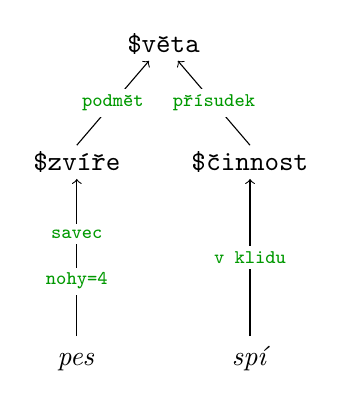
\begin{tikzpicture}[inner sep=2pt]
		\node (pes) at (0, 0) {\strut\emph{pes}};
		\node (spí) at (2.2, 0) {\strut\emph{spí}};
		\node (zvíře) at (0, 2.5) {\texttt{\$zvíře}};
		\node (činnost) at (2.2, 2.5) {\texttt{\$činnost}};
		\node (věta) at (1.1, 4) {\texttt{\$věta}};
		\draw[->] (pes.north) --
		node[pos=0.35, green!60!black,fill=white] {\scriptsize \texttt{nohy=4}}
		node[pos=0.65, green!60!black,fill=white] {\scriptsize \texttt{savec}}
		(zvíře.south);
		\draw[->] (spí.north) -- node[midway,green!60!black, fill=white] {\scriptsize \texttt{v klidu}} (činnost.south);
		\draw[->] (zvíře.north) -- node[midway, green!60!black,fill=white] {\scriptsize \texttt{podmět}} (věta);
		\draw[->] (činnost.north) -- node[midway, green!60!black, fill=white] {\scriptsize \texttt{přísudek}} (věta);
	\end{tikzpicture}
	\hspace{1cm}
	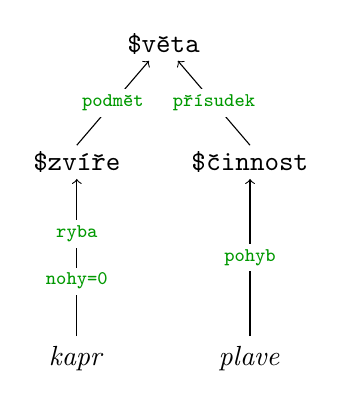
\begin{tikzpicture}[inner sep=2pt]
		\node (kapr) at (0, 0) {\strut\emph{kapr}};
		\node (plave) at (2.2, 0) {\strut\emph{plave}};
		\node (zvíře) at (0, 2.5) {\texttt{\$zvíře}};
		\node (činnost) at (2.2, 2.5) {\texttt{\$činnost}};
		\node (věta) at (1.1, 4) {\texttt{\$věta}};
		\draw[->] (kapr.north) --
		node[pos=0.35, green!60!black,fill=white] {\scriptsize \texttt{nohy=0}}
		node[pos=0.65, green!60!black,fill=white] {\scriptsize \texttt{ryba}}
		(zvíře.south);
		\draw[->] (plave.north) -- node[midway,green!60!black, fill=white] {\scriptsize \texttt{pohyb}} (činnost.south);
		\draw[->] (zvíře.north) -- node[midway, green!60!black,fill=white] {\scriptsize \texttt{podmět}} (věta);
		\draw[->] (činnost.north) -- node[midway, green!60!black, fill=white] {\scriptsize \texttt{přísudek}} (věta);
	\end{tikzpicture}
	\hspace{1cm}
	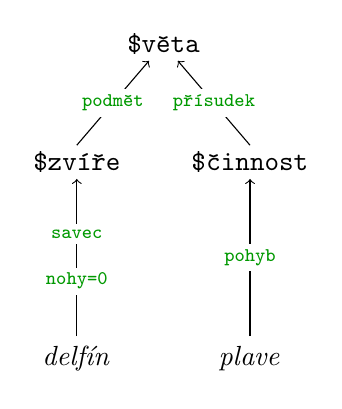
\begin{tikzpicture}[inner sep=2pt]
		\node (delfín) at (0, 0) {\strut\emph{delfín}};
		\node (plave) at (2.2, 0) {\strut\emph{plave}};
		\node (zvíře) at (0, 2.5) {\texttt{\$zvíře}};
		\node (činnost) at (2.2, 2.5) {\texttt{\$činnost}};
		\node (věta) at (1.1, 4) {\texttt{\$věta}};
		\draw[->] (delfín.north) --
		node[pos=0.35, green!60!black,fill=white] {\scriptsize \texttt{nohy=0}}
		node[pos=0.65, green!60!black,fill=white] {\scriptsize \texttt{savec}}
		(zvíře.south);
		\draw[->] (plave.north) -- node[midway,green!60!black, fill=white] {\scriptsize \texttt{pohyb}} (činnost.south);
		\draw[->] (zvíře.north) -- node[midway, green!60!black,fill=white] {\scriptsize \texttt{podmět}} (věta);
		\draw[->] (činnost.north) -- node[midway, green!60!black, fill=white] {\scriptsize \texttt{přísudek}} (věta);
	\end{tikzpicture}
	\caption{Derivační stromy s tagy}\label{fig:derivacni_stromy_tagy}
\end{figure}

Syntaxe SPGF je na Výpise~\ref{lst:spgf_syntax}, detaily implementace je možné
prozkoumat ve zdrojových kódech.
\begin{lstlisting}[
	% there are many more options of styling, see the official documentation, these are just the defaults I like
	frame=single, % make single-line frame around the verbatim
	framesep=2mm, % put some more spacing between the frame and text
	aboveskip=5mm, % put some more space above the box
	basicstyle={\linespread{1.0}\small\ttfamily}, % use typewriter (monospace) font
	caption={Syntaxe SPGF}, % set the caption text
	captionpos=b, % put the caption at the bottom (b) or top (t) or both (bt)
	label={lst:spgf_syntax}, % label to be referenced via \ref{}
	numbers=left, % line numbers on the left
	numberstyle={\scriptsize\ttfamily\color{black!60}}, % the style for line numbers
	escapeinside={<@}{@>} % between those sequences are command evaluated
]
grammar ::= rule+

rule ::= ('public' ' ')? ruleName '=' ruleBody ';'

ruleName ::= '$' unicodeAlphanumerical+

ruleBody ::= ruleAlternative ('|' ruleAlternative)*

ruleAlternative ::= element (' ' element)*

element ::= token | ruleRef | sequence

sequence ::= bracedSequence | optionalSequence

bracedSequence ::= '(' bareSequence ')'

optionalSequence ::= '[' bareSequence ']'

bareSequence ::= ruleAlternative ('|' ruleAlternative)*

token ::= (unicodeAlphanumerical | '.' | '-' | '_' | ':')+ 
          repeatOperator? tag*

repeatOperator ::=  '<' (('L' | 'G' | 'T') ':')? 
             (( digit+ '-' digit* ) | '*' | '+' | '?') '>'

ruleRef ::= '$' ruleName repeatOperator? tag*

tag ::= '{' [^}]+ '}'
\end{lstlisting}


\subsubsection{Parsovací strategie a opakování v SPGF}
Jak bylo zmíněno v sekci~\ref{subsubsec:spgf_def}, v gramatice je možné ke každému elementu,
s výjimkou speciálních pravidel \texttt{\$END}, \texttt{\$BEGIN}, \texttt{\$VOID} a \texttt{\$NULL},
přiřadit definici opakování.

Toto opakování udává, jaký je maximální a minimální počet bezprostředních opakování daného elementu během zpracování textu.
Například pokud má daný token specifikováno, že jeho minimální počet opakování je 2 a maximální 3,
tak v analyzovaném textu bude odpovídající slovo očekáváno dvakrát nebo třikrát po sobě.

Základní syntaxe je převzata ze standardu SRGS,
tedy dvě přirozená čísla oddělená pomlčkou (bez mezer) a ohraničené špičatými závorkami: \enquote{\texttt{<min-max>}}.
Pro pohodlnější zápis bylo definováno několik dalších alternativních
způsobů zápisu, viz Tabulka~\ref{tab:repeat_syntax}.
Pokud element žádné opakování nemá specifikované, implicitní hodnota je 1.

\begin{table}[ht!]
	\centering
	\def\width{14mm}
	\begin{tabular}{|l|p{\width}|p{\width}|l|}
		\hline
		\multirow{2}{*}{\textbf{Syntax}} & \multicolumn{2}{c|}{\textbf{Počet opakování}} & \multirow{2}{*}{\textbf{Poznámka}}                                               \\
		\cline{2-3}
		                                 & \textbf{min}                                  & \textbf{max}                       &                                             \\
		\hline
		\texttt{<m-n>}                   & $m$                                           & $n$                                & $m,n \in \mathbb{N}^{0} \ \wedge \ m\geq n$ \\
		\hline
		\texttt{<m->}                    & $m$                                           & $\infty$                           & v implementaci $\textbf{max} = 2^{32}-1$    \\
		\hline
		\texttt{<m>}                     & $m$                                           & $m$                                & ekvivalentní s \enquote{\texttt{<m-m>}}     \\
		\hline
		\texttt{<*>}                     & $0$                                           & $\infty$                           & ekvivalentní s \enquote{\texttt{<0->}}      \\
		\hline
		\texttt{<+>}                     & $1$                                           & $\infty$                           & ekvivalentní s \enquote{\texttt{<1->}}      \\
		\hline
		\texttt{<?>}                     & $0$                                           & $1$                                & ekvivalentní s \enquote{\texttt{<0-1>}}     \\
		\hline
	\end{tabular}
	\caption{Možné způsoby zápisu opakování v SPGF}\label{tab:repeat_syntax}
\end{table}

S opakovaným použitím stejného elementu je úzce spojena i strategie parsování.
Jedná se o způsob, jakým jsou řešené neurčité situace, kde je možné postupovat vícero způsoby.
Tyto situace mohou vznikat právě v místech opakování elementů, nebo tam, kde je k dispozici vícero aplikovatelných alternativ.

Konkrétní příklad jedné z možných nejednoznačných situací (přímo převzatý ze SRGS specifikace~\cite{srgs}) je v Tabulace~\ref{tab:ambiguity_example}.
Představuje situaci, kdy dvě alternativy mají různé tagy, ale stejné tokeny a tudíž není jasné, kterou z nich použít.
\begin{table}[ht!]
	\centering
	\begin{tabular}{|l|l|}
		\hline
		Expanze            & \texttt{t1 \{tag1\} | t1 \{tag2\} | t2} \\
		Vstupní řetězec    & \texttt{t1}                             \\
		Výstup (možnost 1) & \texttt{[{t1}, \{tag1\}]}               \\
		Výstup (možnost 2) & \texttt{[{t1}, \{tag2\}]}               \\
		\hline
	\end{tabular}
	\caption{Ukázka nejednoznačnosti SRGS}\label{tab:ambiguity_example}
\end{table}

V existující implementaci SRGS, se kterou byly prováděné první experimenty, byl implementován pouze takzvaný \enquote{hladový algoritmus}, běžněji označovaný pod anglickým názvem \emph{greedy matching}.
Pro potřeby sémantické analýzy textu v této práci bylo ovšem zjištěno, že pouze greedy algoritmus nebude zcela postačovat.
\todo{můžu takhle použít rovnou anglické názvy? přijdou mi lepší než české \enquote{hladový} \enquote{líný} nebo \enquote{důsledný}}

Příkladem takové situace by mohla být analýza textu
\begin{center}
	\emph{hnědý pes honí oranžovou malou veverku}
\end{center}
s cílem zjistit vlastnosti objektů (v tomto případě zvířat), zde konkrétně jejich barvy.
Pravidlo pro zachycení barvy zvířete by mohlo vypadat takto:
\begin{center}
	\texttt{public \$has\_color = \$color \$GARBAGE<*> \$animal;}
\end{center}
kde \texttt{\$color} a \texttt{\$animal} jsou reference na pravidla akceptující konkrétní slova pro barvy a zvířata.
Speciální pravidlo \texttt{\$GARBAGE} je zde definováno s operátorem opakování \enquote{\texttt{<*>}},
což lze chápat tak, že mezi samotnou barvou a zvířetem může být libovolný počet dalších slov, která nejsou podstatná.
Při zpracování textu pak ale dochází k problému, že greedy algoritmus vrátí derivační strom zakreslený na Obrázku~\ref{fig:parsing_tree_greedy}:
\begin{figure}[ht!]
	\centering
	\begin{tikzpicture}[inner sep=2pt]
		\def\dist{70pt}
		\foreach \w [count=\wi] in {hnědý, pes, honí, oranžovou, malou, veverku}
		\node (\w) at (\wi*\dist, 0) {\emph{\strut \w}};

		\def\dist{30pt}
		\node (r1) at ($(hnědý.north) + (0, \dist)$) {\strut\texttt{\$color}};
		\node (r2) at ($(pes.north) + (0, \dist)$) {\strut\texttt{\$GARBAGE}};
		\node (r3) at ($(honí.north) + (0, \dist)$) {\strut\texttt{\$GARBAGE}};
		\node (r4) at ($(oranžovou.north) + (0, \dist)$) {\strut\texttt{\$GARBAGE}};
		\node (r5) at ($(malou.north) + (0, \dist)$) {\strut\texttt{\$GARBAGE}};
		\node (r6) at ($(veverku.north) + (0, \dist)$) {\strut\texttt{\$animal}};

		\foreach \w [count=\wi] in {hnědý, pes, honí, oranžovou, malou, veverku}
		\draw[->] (\w.north) -- (r\wi.south);

		\node (color) at ($0.5*(r1.north west) + 0.5*(r6.north east) + (0, 1.5*\dist)$) {\strut \texttt{\$has\_color}};
		\foreach \n in {1,...,6}
		\draw[->] (r\n.north) -- (color);
	\end{tikzpicture}
	\caption{Derivační strom znázorňující problém s greedy algoritmem}\label{fig:parsing_tree_greedy}
\end{figure}

Jak je na derivačním stromu na Obrázku~\ref{fig:parsing_tree_greedy} vidět, následující sémantická analýza by došla pravděpodobně k závěru,
že v textu byla informace o hnědé veverce - což je chyba.
Zde speciální pravidlo \texttt{\$GARBAGE} s neomezeným počtem opakování v kombinaci s greedy algoritmem způsobilo,
že toto speciální pravidlo bylo \enquote{příliš agresivní} a aktivovalo se i v případech, kdy by již bylo možné použít následující element.

Z tohoto důvody byla do systému implementována druhá strategie, která se běžně označuje jako \emph{lazy matching}.
Zatímco greedy matching se v každém okamžiku snaží posunout parsování co nejdále, tato lazy strategie se naopak snaží použít element co nejméněkrát.

Také by se dalo říci, že pokud parsovací algoritmus narazí na element $e_{1}$ následovaný elementem $e_{2}$, pak:
\begin{itemize}
	\item greedy strategie se vždy nejdříve pokusí $e_{1}$ použít (opakovaně po sobě) a postoupí na $e_{2}$ až v moment, kdy
	      již není možné dále opakovat $e_{1}$,
	\item lazy strategie se vždy pokusí nejdříve postoupit na element $e_{2}$ a vrátí se k $e_{1}$ pro opakované použití až v moment,
	      kdy $e_{2}$ není možné použít
\end{itemize}

Implementace lazy strategie umožnila zachytit sémantiku, kterou by bylo obtížné získat pomocí greedy algoritmu.
Po několika dalších experimentech ovšem bylo zjištěno, že ani tato strategie nebude sama o sobě postačovat pro všechny potřeby sémantické analýzy.
Hlavním problémem s lazy strategií bylo to, že v textech, kde bylo více možných vyjádření stejného typu, byla detekována vždy jen ta nejkratší.

\newpage
Například předchozí úloha určování barev zvířat se vstupním textem
\begin{center}
	\emph{velký hnědý pes honí oranžovou malou veverku}
\end{center}
by mohla být zpracována SPGF pravidlem:
\begin{center}
	\texttt{public \$has\_color = \$GARBAGE<*> \$color \$GARBAGE<*> \$animal;}
\end{center}
V tomto případě bylo přidáno na začátek pravidla další \texttt{\$GARBAGE<*>}, které při použití lazy algoritmu způsobí,
že text nemusí začínat přímo barvou, ale je možné hledat barvy a zvířata až později v textu.
Derivační strom tohoto příkladu je zakreslen na Obrázku~\ref{fig:parsing_tree_lazy}.

\begin{figure}[ht!]
	\centering
	\begin{tikzpicture}[inner sep=2pt]
		\def\dist{55pt}
		\foreach \w [count=\wi] in {velký, hnědý, pes, honí, oranžovou, malou, veverku}
		\node (\w) at (\wi*\dist, 0) {\emph{\strut \w}};

		\def\dist{30pt}
		\node (r1) at ($(velký.north) + (0, \dist)$) {\strut\texttt{\$GARBAGE}};
		\node (r2) at ($(hnědý.north) + (0, \dist)$) {\strut\texttt{\$color}};
		\node (r3) at ($(pes.north) + (0, \dist)$) {\strut\texttt{\$animal}};

		\foreach \w [count=\wi] in {velký, hnědý, pes}
		\draw[->] (\w.north) -- (r\wi.south);

		\node (color) at ($0.5*(r1.north west) + 0.5*(r3.north east) + (0, 1.5*\dist)$) {\strut \texttt{\$has\_color}};
		\foreach \n in {1,...,3}
		\draw[->] (r\n.north) -- (color);

		\draw[thick, decorate, decoration={calligraphic brace, amplitude=5}]
		($(honí.north west) + (0, 0)$) -- ($(veverku.north east) + (0, 0)$)
		node[pos=0.5, above=4pt] {\scriptsize zbytek textu (není součástí derivačního stromu)};
	\end{tikzpicture}
	\caption{Derivační strom znázorňující problém s lazy algoritmem}\label{fig:parsing_tree_lazy}
\end{figure}
Z derivačního stromu na Obrázku~\ref{fig:parsing_tree_lazy} je možné usoudit, že následující sémantická analýza by pravděpodobně detekovala,
že v textu se nacházela informace o hnědém psovi - to je správně.
Nicméně je dále možné pozorovat, že v textu se vyskytovala také informace o oranžové veverce, kterou by systém nedokázal takto zachytit.

Z toho důvodu byl implementována ještě třetí strategie, která byla označena jako \enquote{\emph{thorough matching}}.
Myšlenka byla taková, že by bylo vhodné, aby algoritmus v místě nejednoznačnosti nemusel rozhodovat o tom,
který postup je nejlepší, ale aby místo toho uvažoval všechny možnosti.
Tento přístup se tedy od předchozích dvou liší v tom, že může vrátit pro jeden vstup více výstupů.

Základní koncept thorough strategie spočívá v tom, že v místě, kde by bylo možné postupovat vícero způsoby,
je řešení rozděleno do více paralelních větví (jedna pro každou možnost) a každá větev je dále zpracovávána nezávisle.
Tímto způsobem se rekurzivně vytváří strom možných řešení, jehož listy odpovídají finálním derivačním stromům.
Po ukončení všech těchto paralelních parsování jsou úspěšné výsledky vráceny jako seznam derivačních stromů.

Na výstupu tedy bude množina všech možných způsobů, jakým bylo možné derivační strom pro dané pravidlo a vstupní text sestavit.
To následně zaručí, že během zpracování textu nebyla opomenuta žádná sémantika
(za předpokladu, že jsou expertem správně sestavena parsovací pravidla).

Například pro předchozí úlohu určování barev zvířat se vstupním textem
\begin{center}
	\emph{velký hnědý pes honí oranžovou malou veverku}
\end{center}
a SPGF pravidlem:
\begin{center}
	\texttt{public \$has\_color = \$GARBAGE<*> \$color \$GARBAGE<*> \$animal;}
\end{center}
by výstupem byly 3 derivační stromy.
Dva z nich by byly shodné s výstupem greedy a lazy strategie (viz Obrázky~\ref{fig:parsing_tree_greedy} a~\ref{fig:parsing_tree_lazy}),
třetí (nový) derivační strom je na Obrázku~\ref{fig:parsing_tree_thorough}.

\begin{figure}[ht!]
	\centering
	\begin{tikzpicture}[inner sep=2pt]
		\def\dist{62pt}
		\foreach \w [count=\wi] in {velký, hnědý, pes, honí, oranžovou, malou, veverku}
		\node (\w) at (\wi*\dist, 0) {\emph{\strut \w}};

		\def\dist{30pt}
		\node (r1) at ($(velký.north) + (0, \dist)$) {\strut\texttt{\$GARBAGE}};
		\node (r2) at ($(hnědý.north) + (0, \dist)$) {\strut\texttt{\$GARBAGE}};
		\node (r3) at ($(pes.north) + (0, \dist)$) {\strut\texttt{\$GARBAGE}};
		\node (r4) at ($(honí.north) + (0, \dist)$) {\strut\texttt{\$GARBAGE}};
		\node (r5) at ($(oranžovou.north) + (0, \dist)$) {\strut\texttt{\$color}};
		\node (r6) at ($(malou.north) + (0, \dist)$) {\strut\texttt{\$GARBAGE}};
		\node (r7) at ($(veverku.north) + (0, \dist)$) {\strut\texttt{\$animal}};

		\foreach \w [count=\wi] in {velký, hnědý, pes, honí, oranžovou, malou, veverku}
		\draw[->] (\w.north) -- (r\wi.south);

		\node[ellipse] (color) at ($0.5*(r1.north west) + 0.5*(r7.north east) + (0, 1.5*\dist)$) {\strut \texttt{\$has\_color}};
		\foreach \n in {1,...,7}
		\draw[->] (r\n.north) -- (color);
	\end{tikzpicture}
	\caption{Derivační stromy z thorough algoritmu}\label{fig:parsing_tree_thorough}
\end{figure}

Celkově by tedy z tohoto výstupu bylo možné získat informace o tom, že v textu byla hnědá veverka, hnědý pes a oranžová veverka.
Dvě z těchto informací jsou správně, pouze informace o hnědé veverce je chybná, ta se v textu nevyskytla.

Jedná se o jednu z nevýhod thorough přístupu, že bude v textu hledat i takové informace, které z něj neplynou.
Tento problém byl vyřešen následnou filtrací získaných entit oproti referenčnímu popisu.
Detailní popis tohoto filtrování bude popsán v kapitole~\ref{subsubsec:algoritmus_zpracovani_stromu}.
% tak, že získané sémantické informace jsou porovnané s referenčním popisem obrázku a ty,
% které se v referenčním popise nevyskytují, jsou považované za falešně detekované a jsou z výstupu odstraněné
% (s výjimkou hodnot atributů, řešení chybných hodnot je popsáno v kapitole~\ref{subsec:hodnoceni}).

Tímto způsobem je pak v testovaném popisu pouze podmnožina referenčního popisu.
Jedná se o jednoduchý a efektivní způsob řešení falešně detekovaných sémantických informací.
Také ale bohužel představuje omezení v tom smyslu, že neumožňuje detekovat sémantiku, která se v textu skutečně nacházela,
ale nebyla zanesena do referenčního popisu - to klade očekávání na kvalitu referenčního popisu od experta.
Sestavení nějakého složitějšího algoritmu pro detekci falešně extrahované sémantiky představuje jedno z možných rozšíření do budoucna.

Další nevýhodou thorough strategie je její výpočetní náročnost.
Vzhledem k rekurzivnímu charakteru algoritmu a způsobu vytváření nových paralelních větví
se naskýtá riziko kombinatorické exploze počtu paralelních větví.
Během testování se však ukázalo, že pro moderní výpočetní techniku nepředstavují vstupy o velikosti desítek až stovek tokenů žádný problém.
Detailnější analýza výpočetní a paměťové náročnosti pro větší vstupy je nad rámec zadání a byla ponechána pro budoucí práce.

Posledním problémem, který bylo potřeba vyřešit v rámci parsovacích strategií, byl způsob, jakým strategie volit a přepínat.
V první verzi parseru se jednalo o globální přepínač, kdy bylo možné před samotným parsováním zvolit, jaká strategie má být použita.
Bylo ale zjištěno, že pro některé situace by bylo výhodné, aby bylo možné změnit výchozí strategii pro konkrétní pravidla nebo jejich části.

Například při zpracovávání číselných údajů je vhodná greedy strategie.
Je totiž potřeba, aby posloupnost sobě jdoucí slov, které reprezentující číselný údaj, byla brána jako jeden celek.

Jiný příklad pak může být již výše zmíněný začátek pravidla \texttt{\$GARBAGE<*>},
který libovolný počet prvních slov považovat za výplň a hledat tak význam až později v textu.
Pro tuto situaci je naopak greedy algoritmus zcela nevhodný, protože by celý text byl zpracován hned tímto počátkem.
Zde je vhodná lazy strategie, která ve své podstatě bude dávat přednost následujícím elementům
v pravidle a tento počátek bude používat až když zbytek pravidla selže.

Z těchto důvodů byla rozšířena syntaxe pro operátor definující opakování.
Před samotné hodnoty opakování (tedy hned za otevírací špičatou závorku \enquote{\texttt{<}}) je možné napsat
jedno z písmen \texttt{L}, \texttt{G}, \texttt{T} následované dvojtečkou a poté zbytek definice opakování.
Tato písmena odpovídají jednotlivým strategiím (lazy, greedy, thorough) a umožňují tak vynutit danou strategii pro dané pravidlo nebo jeho část.
Ve výsledku tak operátor opakování může vypadat například \enquote{\texttt{<G:1-3>}}, \enquote{\texttt{<L:*>}}, nebo \enquote{\texttt{<T:2->}}.

\subsection{Tvorba testovaného popisu}
Po implementaci systému pro zpracování přirozeného textu pomocí bezkontextových gramatik bylo potřeba získané derivační stromy nějakým způsobem
zpracovat a vytvořit z nich testovaný popis, který by bylo možné srovnat s referenčním popisem od experta.

Zpracování derivačních stromů obecně představuje konflikt mezi obtížností automatického zpracování a omezením na strukturu.
Striktně daná forma bude lépe zpracovatelná programově, ale může být obtížné zachytit všechny potřebné informace v dané struktuře.
Naopak více volná forma bude umožňovat snadnější zachycení různých typů informace, ale bude obtížnější sestavit algoritmus,
který by dokázal spolehlivě zpracovat předem neznámou strukturu.

Vzhledem k podobě testovaného a referenčního popisu, které byly popsané v kapitole~\ref{sec:navrh_architektura},
byl vytvořen algoritmus, který prochází získané derivační stromy a ukládá navštívené uzly s tagy do seznamu.
Z tohoto seznamu tagů pak určuje, jaká sémantická informace je v derivačním stromu obsažena.

Zde navržený přístup klade požadavek na způsob, jakým jsou sestavené SPGF gramatiky, protože předpokládá, že výstupní derivační stromy
budou mít takovou strukturu, aby při jejich procházení byly nalezené tagy v očekávaném pořadí.
Neklade tedy omezení přímo na strukturu samotných derivačních stromů, ale pouze na relativní rozmístění tagů uvnitř derivačního stromu.

\subsubsection{Algoritmus zpracování derivačních stromů}\label{subsubsec:algoritmus_zpracovani_stromu}
V první fázi algoritmus projde získaný derivační strom $T$ strategií depth-first-post-order (dfpo)~\cite{taocp1} a všechny navštívené tagy $t_{i}$ ukládá do seznamu.
Index $i$ značí index tagu odpovídající jeho pořadí při dfpo procházení stromu $T$.

Příklad takového stromu je na Obrázku~\ref{fig:tree_example}.
Zde je možné vidět, že ve skutečnosti tagy jsou realizované jako samostatné uzly, které následují vždy jako poslední (zleva doprava) uzel ke svému rodičovskému uzlu.
Při dfpo zpracování pak z tohoto stromu vznikne následující posloupnost tagů:
\begin{center}
	\texttt{[dog, part=obj, squirrel, part=subj, predicate=chasing, type=triplet]}
\end{center}

\begin{figure}[H]
	\centering
	\begin{tikzpicture}[inner sep=0pt,every node/.style={}]
		\def\dist{60pt}
		\foreach \w [count=\wi] in {velký, hnědý, pes, honí, oranžovou, malou, veverku}
		\node (\w) at (\wi*\dist, 0) {\emph{\strut \w}};

		\node (dog) at ($(pes.north) + (0, 50pt)$) {\strut\texttt{\$dog}};
		\node (g1) at ($(velký.north) + (0, 50pt)$) {\strut\texttt{\$GARBAGE}};
		\node (g2) at ($(hnědý.north) + (0, 50pt)$) {\strut\texttt{\$GARBAGE}};
		\node (obj1) at ($(dog.north) + (24pt, 50pt)$) {\strut\texttt{\$object}};
		\node (chasing) at ($(obj1.north) + (82pt, 50pt)$) {\strut\texttt{\$chasing}};
		\node (g3) at ($(oranžovou.north) + (0pt, 50pt)$) {\strut\texttt{\$GARBAGE}};
		\node (g4) at ($(malou.north) + (0, 50pt)$) {\strut\texttt{\$GARBAGE}};
		\node (squirrel) at ($(veverku.north) + (0, 50pt)$) {\strut\texttt{\$squirrel}};
		\node (obj2) at ($(squirrel.north) + (-60pt, 50pt)$) {\strut\texttt{\$object}};
		\node (triplet) at ($(chasing.north) + (0, 50pt)$) {\strut\texttt{\$triplet}};
		\node (output) at ($(triplet.north) + (-1, 50pt)$) {\strut\texttt{\$output}};

		\node[green!60!black, anchor=north west] (t1) at ($(dog.south east) + (0pt, -15pt)$) {\footnotesize\strut dog};
		\node[green!60!black, anchor=north west] (t2) at ($(obj1.south east) + (-26pt, -20pt)$) {\footnotesize\strut part=obj};
		\node[green!60!black, anchor=north west] (t3) at ($(squirrel.south east) + (-17.6pt, -15pt)$) {\footnotesize\strut squirrel};
		\node[green!60!black, anchor=north west] (t4) at ($(obj2.south east) + (30pt, -15pt)$) {\footnotesize\strut part=subj};
		\node[green!60!black, anchor=north west] (t5) at ($(chasing.south east) + (53pt, -19pt)$) {\footnotesize\strut predicate=chasing};
		\node[green!60!black, anchor=north west] (t6) at ($(triplet.south east) + (0pt, -15pt)$) {\footnotesize\strut type=triplet};
		\draw[-](t1) -- (dog);
		\draw[-](t2) -- (obj1);
		\draw[-](t3) -- (squirrel);
		\draw[-](t4) -- (obj2);
		\draw[-](t5) -- (chasing);
		\draw[-](t6) -- (triplet);

		\draw[-] (velký) to (g1);
		\draw[-] (hnědý) to (g2);
		\draw[-] (pes) to (dog);
		\draw[-] (honí) to (chasing);
		\draw[-] (oranžovou) to (g3);
		\draw[-] (malou) to (g4);
		\draw[-] (veverku) to (squirrel);
		\draw[-] (dog) to (obj1);
		\draw[-] (squirrel) to (obj2);
		\draw[-] (obj1) to (chasing);
		\draw[-] (obj2) to (chasing);
		\draw[-] (g3) to (chasing);
		\draw[-] (g4) to (chasing);
		\draw[-] (chasing) to (triplet);
		\draw[-] (triplet) to (output);
		\draw[-] (g1) to (output);
		\draw[-] (g2) to (output);

	\end{tikzpicture}
	\caption{Příklad derivačního stromu s tagy pro zpracování}\label{fig:tree_example}
\end{figure}

Získaný seznam tagů je postupně porovnáván s jednotlivými vzory, zda odpovídá nějaké předem definované sémantické informaci.
Rozlišované jsou tři typy informací, které odpovídají struktuře referenčního a testovaného popisu:
\begin{enumerate}
	\item \textbf{Objekty}: \\
	      Pro objekty stačí pouze identifikátor toho, že se jedná o objekt, a poté samotný název objektu.
	      Očekávaný seznam tagů tedy musí mít následující strukturu:
	      \begin{center}
		      $\bigl[ $ \emph{name},\ {\texttt{type=object}} $\bigr]$
	      \end{center}
	      kde \emph{name} je libovolný řetězec, který bude považován za název objektu.

	      Například při zpracování derivačního stromu, ze kterého bude získána posloupnost tagů
	      \texttt{[dog, type=object]},
	      bude extrahován objekt \enquote{\emph{dog}}, který bude poté přidán do testovaného popisu.
	\item \textbf{Atributy}: \\
	      Pro kompletní určení atributu je třeba identifikátor toho, že se jedná o atribut,
	      pak objekt, kterému je atribut přiřazen, následně název atributu a jeho hodnota.
	      Pro extrakci atributů byly definovány dvě různé struktury, kterých může seznam tagů nabývat:
	      \begin{center}
		      $\bigl[$ \emph{o\_name}, {\texttt{part=obj}}, \emph{a\_val}, \emph{a\_name},
					      {\texttt{part=attr}}, {\texttt{type=attribute}} $\bigr]$ \\
		      $\bigl[$ \emph{a\_val}, \emph{a\_name}, {\texttt{part=attr}}, \emph{o\_name},
					      {\texttt{part=obj}}, {\texttt{type=attribute}} $\bigr]$
	      \end{center}
	      kde \emph{o\_name}, \emph{a\_val} a \emph{a\_name} jsou libovolné řetězce, které budou považované za název objektu,
	      hodnotu atributu a název atributu.

	      Dvě různá očekávaná pořadí tagů vycházejí z toho, že v běžné mluvě lze specifikovat vlastnost objektu
	      před objektem (např.~\enquote{\emph{hnědý pes}}) i po něm (např.~\enquote{\emph{pes je hnědý}}).

	      Například při zpracování derivačního stromu, ze kterého budou získány tagy
	      \begin{center}
		      \texttt{[dog, part=obj, brown, color, part=attr, type=attribute]},
	      \end{center}
	      bude extrahován atribut \enquote{\emph{dog: color = brown}}, který bude poté přidán do testovaného popisu.
	\item \textbf{Vazby mezi objekty}:\\
	      Pro kompletní určení vazby mezi dvěma objekty je potřeba znát názvy obou objektů a název vazby mezi nimi.
	      Pro extrakci vazeb mezi objekty je očekáváno následující pořadí tagů:
	      \begin{center}
		      $\bigl[ $ \emph{from}, \texttt{part=obj}, \emph{to},
					      {\texttt{part=subj}}, \texttt{predicate=}\emph{pred}, {\texttt{type=triplet}} $\bigr]$
	      \end{center}
	      kde \emph{from}, \emph{to} a \emph{pred} jsou libovolné řetězce, které budou považované za název
	      zdrojového objektu, cílového objektu a název vazby.

	      Například při zpracování derivačního stromu, ze kterého budou získány tagy
	      \begin{center}
		      \texttt{[dog, part=obj, squirrel, part=subj, predicate=chasing, type=triplet]},
	      \end{center}
	      bude extrahován triplet \enquote{\emph{dog chasing squirrel}}, který bude poté přidán do testovaného popisu.
\end{enumerate}

Po extrakci objektů, atributů a tripletů jsou tyto získané sémantické informace profiltrovány,
za cílem odstranění falešně detekovaných entit.
Jak již bylo dříve zmíněno, filtrování probíhá tím způsobem, že pokud daný objekt, atribut,
nebo triplet nejsou v referenčním popisu, jsou ze seznamu odstraněné.
Výjimku tvoří atributy, kde je pouze chybná hodnota - tyto atributy jsou v seznamu ponechané a jsou uvažované v hodnocení,
jak bylo popsáno v kapitole~\ref{subsec:hodnoceni}.

\subsubsection{Číslování objektů}\label{subsubsec:cislovani_objektu}
Jeden z problémů, na který byl během implementace objeven, je absence číslování objektů.
Jak bylo popsáno v sekci~\ref{subsec:referencni_popis}, objekty mohou mít v rámci svého názvu číslování, kvůli jednoznačné rozlišitelnosti.
Nelze předpokládat, že by se tato číselná informace jakkoli vyskytovala v přirozeném popisu.
Naskýtá se tedy otázka, jak z přirozeného textu získat informaci o tom, o který objekt se konkrétně jedná
(za předpokladu, že daný objekt je v referenčním popise číslován).

Pro tento účel rozlišení číslovaných objektů byl sestaven doplňkový algoritmus,
který využívá unikátních vlastností objektů a jejich vazeb.
Hlavní myšlenka spočívá v tom, že pokud se názvy vícero objektů liší pouze číslováním,
pak je možné využít jejich atributy a vlastnosti k rozlišení, který objekt je který.

Například pokud ve scéně budou dva stromy \enquote{\texttt{strom \#1}} a \enquote{\texttt{strom \#2}} a právě jeden z nich
bude součástí tripletu \enquote{\texttt{veverka \to\ šplhá\_po \to\ strom \#1}}, pak lze například z textu:
\begin{center}
	\enquote{\emph{na obrázku vidím veverku, co šplhá po stromě}}
\end{center}
usoudit, že se jedná o \enquote{\texttt{strom \#1}}, protože \enquote{\texttt{strom \#2}} nemůže být součástí daného tripletu.
Je zde opět použit optimistický přístup, který předpokládá, že uživatel skutečně měl na mysli ten daný objekt (v tomto případě strom),
který se vyskytuje v detekovaném atributu či tripletu.

Na tomto principu byl tedy implementován algoritmus, který iterativně prochází extrahované informace z derivačních stromů
a postupně hledá, zda jsou v datech nějaké objekty, které by šly takto specifikovat.
Pokud je nějaký takový objekt nalezen, pak je mu přidáno příslušné číslování nejen v daném atributu nebo tripletu,
ale i ve všech ostatních extrahovaných datech, jelikož si vnitřní implementace udržuje informace o tom,
ze které části textu který kousek sémantiky pochází.

Dále se může stát, že specifikování jednoho objektu umožní následovné specifikování jiného objektu, protože dojde k eliminaci ostatních možností.
Tento iterativní algoritmus tedy prochází opakovaně všechna extrahovaná data až do chvíle,
než je celý průchod beze změny - v ten okamžik proces končí.

\subsection{Hodnotící algoritmus a ztrátová tabulka}
Po získání testovaného popisu je potřeba jej srovnat s referenčním popisem a ohodnotit míru jejich shody.
K tomuto účelu byl navržen a implementován hodnotící algoritmus, který byl detailně popsán v kapitole~\ref{subsec:hodnoceni}.

Vstupem jsou referenční popis získaný od experta, testovaný popis, jehož získání je popsáno v předchozích kapitolách a ztrátová tabulka,
která udává závažnost různých chyb.
Samotná ztrátová tabulka odpovídá svým formátem asociativnímu poli (též hash-tabulka nebo slovník), s předem danou strukturou.
Jelikož je SPGF systém citlivý na velikost písmen a interpunkční znaménka, jsou texty před vstupem normalizované
a zpracovávané větu po větě, výsledky pro jednotlivé věty jsou na konči sloučené.

Jak již bylo řečeno v kapitole~\ref{subsec:hodnoceni}, ztrátovou tabulku sestavuje expert, stejně jako referenční popis a SPGF gramatiky.
Z toho důvodu bylo nutné zvolit nějaký formát, který by byl čitelný člověkem a zároveň zpracovatelný strojem.
Zvolen byl opět formát \texttt{JSON}, který představuje dobrý kompromis mezi oběma faktory.
Ukázka ztrátové tabulky je na Výpisu~\ref{lst:loss_table_example}.

\begin{lstlisting}[
	% there are many more options of styling, see the official documentation, these are just the defaults I like
	frame=single, % make single-line frame around the verbatim
	framesep=2mm, % put some more spacing between the frame and text
	aboveskip=5mm, % put some more space above the box
	basicstyle={\linespread{0.9}\small\ttfamily}, % use typewriter (monospace) font
	caption={Ztrátová tabulka použitá při testování}, % set the caption text
	captionpos=b, % put the caption at the bottom (b) or top (t) or both (bt)
	label={lst:loss_table_example}, % label to be referenced via \ref{}
	numbers=left, % line numbers on the left
	numberstyle={\scriptsize\ttfamily\color{black!60}}, % the style for line numbers
	escapeinside={<@}{@>} % between those sequences are command evaluated
]
<@\textcolor[HTML]{FF1010}{\texttt{\{}}@>
<@\textcolor[HTML]{000000}{\texttt{\ \ }}@><@\textcolor[HTML]{255CFF}{\texttt{"missing\_objects"}}@><@\textcolor[HTML]{1041FF}{\texttt{:}}@><@\textcolor[HTML]{000000}{\texttt{\ }}@><@\textcolor[HTML]{DE6F10}{\texttt{3}}@><@\textcolor[HTML]{1041FF}{\texttt{,}}@>
<@\textcolor[HTML]{000000}{\texttt{\ \ }}@><@\textcolor[HTML]{255CFF}{\texttt{"missing\_attributes"}}@><@\textcolor[HTML]{1041FF}{\texttt{:}}@><@\textcolor[HTML]{000000}{\texttt{\ }}@><@\textcolor[HTML]{DE6F10}{\texttt{1}}@><@\textcolor[HTML]{1041FF}{\texttt{,}}@>
<@\textcolor[HTML]{000000}{\texttt{\ \ }}@><@\textcolor[HTML]{255CFF}{\texttt{"missing\_triplets"}}@><@\textcolor[HTML]{1041FF}{\texttt{:}}@><@\textcolor[HTML]{000000}{\texttt{\ }}@><@\textcolor[HTML]{DE6F10}{\texttt{2}}@><@\textcolor[HTML]{1041FF}{\texttt{,}}@>
<@\textcolor[HTML]{000000}{\texttt{\ \ }}@><@\textcolor[HTML]{255CFF}{\texttt{"numberless\_penalty"}}@><@\textcolor[HTML]{1041FF}{\texttt{:}}@><@\textcolor[HTML]{000000}{\texttt{\ }}@><@\textcolor[HTML]{DE6F10}{\texttt{0.5}}@><@\textcolor[HTML]{1041FF}{\texttt{,}}@>
<@\textcolor[HTML]{000000}{\texttt{\ \ }}@><@\textcolor[HTML]{255CFF}{\texttt{"wrong\_values"}}@><@\textcolor[HTML]{1041FF}{\texttt{:}}@><@\textcolor[HTML]{000000}{\texttt{\ }}@><@\textcolor[HTML]{DE6F10}{\texttt{2}}@><@\textcolor[HTML]{1041FF}{\texttt{,}}@>
<@\textcolor[HTML]{000000}{\texttt{\ \ }}@><@\textcolor[HTML]{255CFF}{\texttt{"missing\_objects\_override"}}@><@\textcolor[HTML]{1041FF}{\texttt{:}}@><@\textcolor[HTML]{000000}{\texttt{\ }}@><@\textcolor[HTML]{FF1010}{\texttt{[}}@>
<@\textcolor[HTML]{000000}{\texttt{\ \ \ \ }}@><@\textcolor[HTML]{FF1010}{\texttt{[}}@><@\textcolor[HTML]{418310}{\texttt{"person"}}@><@\textcolor[HTML]{1041FF}{\texttt{,}}@><@\textcolor[HTML]{000000}{\texttt{\ }}@><@\textcolor[HTML]{DE6F10}{\texttt{5}}@><@\textcolor[HTML]{FF1010}{\texttt{]}}@><@\textcolor[HTML]{1041FF}{\texttt{,}}@>
<@\textcolor[HTML]{000000}{\texttt{\ \ \ \ }}@><@\textcolor[HTML]{FF1010}{\texttt{[}}@><@\textcolor[HTML]{418310}{\texttt{"animal"}}@><@\textcolor[HTML]{1041FF}{\texttt{,}}@><@\textcolor[HTML]{000000}{\texttt{\ }}@><@\textcolor[HTML]{DE6F10}{\texttt{4}}@><@\textcolor[HTML]{FF1010}{\texttt{]}}@><@\textcolor[HTML]{1041FF}{\texttt{,}}@>
<@\textcolor[HTML]{000000}{\texttt{\ \ \ \ }}@><@\textcolor[HTML]{FF1010}{\texttt{[}}@><@\textcolor[HTML]{418310}{\texttt{"environment"}}@><@\textcolor[HTML]{1041FF}{\texttt{,}}@><@\textcolor[HTML]{000000}{\texttt{\ }}@><@\textcolor[HTML]{DE6F10}{\texttt{1}}@><@\textcolor[HTML]{FF1010}{\texttt{]}}@>
<@\textcolor[HTML]{000000}{\texttt{\ \ }}@><@\textcolor[HTML]{FF1010}{\texttt{]}}@><@\textcolor[HTML]{1041FF}{\texttt{,}}@>
<@\textcolor[HTML]{000000}{\texttt{\ \ }}@><@\textcolor[HTML]{255CFF}{\texttt{"missing\_attributes\_override"}}@><@\textcolor[HTML]{1041FF}{\texttt{:}}@><@\textcolor[HTML]{000000}{\texttt{\ }}@><@\textcolor[HTML]{FF1010}{\texttt{[}}@>
<@\textcolor[HTML]{000000}{\texttt{\ \ \ \ }}@><@\textcolor[HTML]{FF1010}{\texttt{[}}@><@\textcolor[HTML]{418310}{\texttt{"action"}}@><@\textcolor[HTML]{1041FF}{\texttt{,}}@><@\textcolor[HTML]{000000}{\texttt{\ }}@><@\textcolor[HTML]{DE6F10}{\texttt{1.5}}@><@\textcolor[HTML]{FF1010}{\texttt{]}}@><@\textcolor[HTML]{1041FF}{\texttt{,}}@>
<@\textcolor[HTML]{000000}{\texttt{\ \ \ \ }}@><@\textcolor[HTML]{FF1010}{\texttt{[}}@><@\textcolor[HTML]{418310}{\texttt{"state"}}@><@\textcolor[HTML]{1041FF}{\texttt{,}}@><@\textcolor[HTML]{000000}{\texttt{\ }}@><@\textcolor[HTML]{DE6F10}{\texttt{0.5}}@><@\textcolor[HTML]{FF1010}{\texttt{]}}@>
<@\textcolor[HTML]{000000}{\texttt{\ \ }}@><@\textcolor[HTML]{FF1010}{\texttt{]}}@><@\textcolor[HTML]{1041FF}{\texttt{,}}@>
<@\textcolor[HTML]{000000}{\texttt{\ \ }}@><@\textcolor[HTML]{255CFF}{\texttt{"missing\_triplets\_override"}}@><@\textcolor[HTML]{1041FF}{\texttt{:}}@><@\textcolor[HTML]{000000}{\texttt{\ }}@><@\textcolor[HTML]{FF1010}{\texttt{[}}@><@\textcolor[HTML]{FF1010}{\texttt{[}}@><@\textcolor[HTML]{418310}{\texttt{"falling\ into"}}@><@\textcolor[HTML]{1041FF}{\texttt{,}}@><@\textcolor[HTML]{000000}{\texttt{\ }}@><@\textcolor[HTML]{DE6F10}{\texttt{5}}@><@\textcolor[HTML]{FF1010}{\texttt{]}}@><@\textcolor[HTML]{FF1010}{\texttt{]}}@><@\textcolor[HTML]{1041FF}{\texttt{,}}@>
<@\textcolor[HTML]{000000}{\texttt{\ \ }}@><@\textcolor[HTML]{255CFF}{\texttt{"wrong\_values\_override"}}@><@\textcolor[HTML]{1041FF}{\texttt{:}}@><@\textcolor[HTML]{000000}{\texttt{\ }}@><@\textcolor[HTML]{FF1010}{\texttt{[}}@>
<@\textcolor[HTML]{000000}{\texttt{\ \ \ \ }}@><@\textcolor[HTML]{FF1010}{\texttt{\{}}@>
<@\textcolor[HTML]{000000}{\texttt{\ \ \ \ \ \ }}@><@\textcolor[HTML]{255CFF}{\texttt{"attribute"}}@><@\textcolor[HTML]{1041FF}{\texttt{:}}@><@\textcolor[HTML]{000000}{\texttt{\ }}@><@\textcolor[HTML]{418310}{\texttt{"color"}}@><@\textcolor[HTML]{1041FF}{\texttt{,}}@>
<@\textcolor[HTML]{000000}{\texttt{\ \ \ \ \ \ }}@><@\textcolor[HTML]{255CFF}{\texttt{"default"}}@><@\textcolor[HTML]{1041FF}{\texttt{:}}@><@\textcolor[HTML]{000000}{\texttt{\ }}@><@\textcolor[HTML]{DE6F10}{\texttt{0.5}}@><@\textcolor[HTML]{1041FF}{\texttt{,}}@>
<@\textcolor[HTML]{000000}{\texttt{\ \ \ \ \ \ }}@><@\textcolor[HTML]{255CFF}{\texttt{"overrides"}}@><@\textcolor[HTML]{1041FF}{\texttt{:}}@><@\textcolor[HTML]{000000}{\texttt{\ }}@><@\textcolor[HTML]{FF1010}{\texttt{[}}@>
<@\textcolor[HTML]{000000}{\texttt{\ \ \ \ \ \ \ \ }}@><@\textcolor[HTML]{FF1010}{\texttt{[}}@><@\textcolor[HTML]{FF1010}{\texttt{[}}@><@\textcolor[HTML]{418310}{\texttt{"white"}}@><@\textcolor[HTML]{1041FF}{\texttt{,}}@><@\textcolor[HTML]{000000}{\texttt{\ }}@><@\textcolor[HTML]{418310}{\texttt{"yellow"}}@><@\textcolor[HTML]{1041FF}{\texttt{,}}@><@\textcolor[HTML]{000000}{\texttt{\ }}@><@\textcolor[HTML]{418310}{\texttt{"pink"}}@><@\textcolor[HTML]{FF1010}{\texttt{]}}@><@\textcolor[HTML]{1041FF}{\texttt{,}}@><@\textcolor[HTML]{000000}{\texttt{\ }}@><@\textcolor[HTML]{DE6F10}{\texttt{0.3}}@><@\textcolor[HTML]{FF1010}{\texttt{]}}@><@\textcolor[HTML]{1041FF}{\texttt{,}}@>
<@\textcolor[HTML]{000000}{\texttt{\ \ \ \ \ \ \ \ }}@><@\textcolor[HTML]{FF1010}{\texttt{[}}@><@\textcolor[HTML]{FF1010}{\texttt{[}}@><@\textcolor[HTML]{418310}{\texttt{"red"}}@><@\textcolor[HTML]{1041FF}{\texttt{,}}@><@\textcolor[HTML]{000000}{\texttt{\ }}@><@\textcolor[HTML]{418310}{\texttt{"blue"}}@><@\textcolor[HTML]{1041FF}{\texttt{,}}@><@\textcolor[HTML]{000000}{\texttt{\ }}@><@\textcolor[HTML]{418310}{\texttt{"green"}}@><@\textcolor[HTML]{1041FF}{\texttt{,}}@><@\textcolor[HTML]{000000}{\texttt{\ }}@><@\textcolor[HTML]{418310}{\texttt{"yellow"}}@><@\textcolor[HTML]{FF1010}{\texttt{]}}@><@\textcolor[HTML]{1041FF}{\texttt{,}}@><@\textcolor[HTML]{000000}{\texttt{\ }}@><@\textcolor[HTML]{DE6F10}{\texttt{0.8}}@><@\textcolor[HTML]{FF1010}{\texttt{]}}@>
<@\textcolor[HTML]{000000}{\texttt{\ \ \ \ \ \ }}@><@\textcolor[HTML]{FF1010}{\texttt{]}}@>
<@\textcolor[HTML]{000000}{\texttt{\ \ \ \ }}@><@\textcolor[HTML]{FF1010}{\texttt{\}}}@><@\textcolor[HTML]{1041FF}{\texttt{,}}@>
<@\textcolor[HTML]{000000}{\texttt{\ \ \ \ }}@><@\textcolor[HTML]{FF1010}{\texttt{\{}}@>
<@\textcolor[HTML]{000000}{\texttt{\ \ \ \ \ \ }}@><@\textcolor[HTML]{255CFF}{\texttt{"attribute"}}@><@\textcolor[HTML]{1041FF}{\texttt{:}}@><@\textcolor[HTML]{000000}{\texttt{\ }}@><@\textcolor[HTML]{418310}{\texttt{"action"}}@><@\textcolor[HTML]{1041FF}{\texttt{,}}@>
<@\textcolor[HTML]{000000}{\texttt{\ \ \ \ \ \ }}@><@\textcolor[HTML]{255CFF}{\texttt{"default"}}@><@\textcolor[HTML]{1041FF}{\texttt{:}}@><@\textcolor[HTML]{000000}{\texttt{\ }}@><@\textcolor[HTML]{DE6F10}{\texttt{1.5}}@><@\textcolor[HTML]{1041FF}{\texttt{,}}@>
<@\textcolor[HTML]{000000}{\texttt{\ \ \ \ \ \ }}@><@\textcolor[HTML]{255CFF}{\texttt{"overrides"}}@><@\textcolor[HTML]{1041FF}{\texttt{:}}@><@\textcolor[HTML]{000000}{\texttt{\ }}@><@\textcolor[HTML]{FF1010}{\texttt{[}}@>
<@\textcolor[HTML]{000000}{\texttt{\ \ \ \ \ \ \ \ }}@><@\textcolor[HTML]{FF1010}{\texttt{[}}@><@\textcolor[HTML]{FF1010}{\texttt{[}}@><@\textcolor[HTML]{418310}{\texttt{"sitting"}}@><@\textcolor[HTML]{1041FF}{\texttt{,}}@><@\textcolor[HTML]{000000}{\texttt{\ }}@><@\textcolor[HTML]{418310}{\texttt{"reading"}}@><@\textcolor[HTML]{FF1010}{\texttt{]}}@><@\textcolor[HTML]{1041FF}{\texttt{,}}@><@\textcolor[HTML]{000000}{\texttt{\ }}@><@\textcolor[HTML]{DE6F10}{\texttt{0.8}}@><@\textcolor[HTML]{FF1010}{\texttt{]}}@><@\textcolor[HTML]{1041FF}{\texttt{,}}@>
<@\textcolor[HTML]{000000}{\texttt{\ \ \ \ \ \ \ \ }}@><@\textcolor[HTML]{FF1010}{\texttt{[}}@><@\textcolor[HTML]{FF1010}{\texttt{[}}@><@\textcolor[HTML]{418310}{\texttt{"fishing"}}@><@\textcolor[HTML]{1041FF}{\texttt{,}}@><@\textcolor[HTML]{000000}{\texttt{\ }}@><@\textcolor[HTML]{418310}{\texttt{"sitting"}}@><@\textcolor[HTML]{FF1010}{\texttt{]}}@><@\textcolor[HTML]{1041FF}{\texttt{,}}@><@\textcolor[HTML]{000000}{\texttt{\ }}@><@\textcolor[HTML]{DE6F10}{\texttt{0.7}}@><@\textcolor[HTML]{FF1010}{\texttt{]}}@>
<@\textcolor[HTML]{000000}{\texttt{\ \ \ \ \ \ }}@><@\textcolor[HTML]{FF1010}{\texttt{]}}@>
<@\textcolor[HTML]{000000}{\texttt{\ \ \ \ }}@><@\textcolor[HTML]{FF1010}{\texttt{\}}}@>
<@\textcolor[HTML]{000000}{\texttt{\ \ }}@><@\textcolor[HTML]{FF1010}{\texttt{]}}@>
<@\textcolor[HTML]{FF1010}{\texttt{\}}}@>

\end{lstlisting}


Význam jednotlivých položek byl detailně popsán v sekci~\ref{subsec:hodnoceni}, proto zde bude pouze stručně shrnuto,
který klíč odpovídá jakému významu:
\begin{itemize}
	\item \texttt{missing\_objects} \to\ výchozí ztráta pro chybějící objekty
	\item \texttt{missing\_attributes} \to\ výchozí ztráta pro chybějící atributy
	\item \texttt{missing\_triplets} \to\ výchozí ztráta pro chybějící triplety (vazby)
	\item \texttt{numberless\_penalty} \to\ ztráta pro informace obsahující objekty s chybějícím číslováním (viz sekce~\ref{subsubsec:cislovani_objektu})
	\item \texttt{wrong\_value} \to\ výchozí ztráta pro atributy s chybnou hodnotou
	\item \texttt{missing\_objects\_override} \to\ seznam konkrétních ztrát pro chybějící objekty s daným tagem
	\item \texttt{missing\_attributes\_override} \to\ seznam konkrétních ztrát pro chybějící atributy (podle názvu atributu)
	\item \texttt{missing\_triplets\_override} \to\ seznam konkrétních ztrát pro chybějící triplety (podle názvu vazby)
	\item \texttt{wrong\_values\_override} \to\ seznam konkrétních ztrát pro daný atribut a případně i pro záměnu konkrétních hodnot
\end{itemize}

Finálním výstupem hodnotícího algoritmu je množina označených číselných hodnot, získaných akumulací ztrát pro různé druhy chyb.
Přirozenou datovou strukturou, která by odpovídala tomuto formátu, by bylo asociativní pole (někdy také označované jako hash-tabulka, nebo slovník).

Příkladem takového výstupu může být Výpis~\ref{lst:output_example}:
\begin{lstlisting}[
	% there are many more options of styling, see the official documentation, these are just the defaults I like
	frame=single, % make single-line frame around the verbatim
	framesep=2mm, % put some more spacing between the frame and text
	aboveskip=5mm, % put some more space above the box
	basicstyle={\linespread{0.9}\small\ttfamily}, % use typewriter (monospace) font
	caption={Ukázka výpisu hodnocení (zkráceno)}, % set the caption text
	captionpos=b, % put the caption at the bottom (b) or top (t) or both (bt)
	label={lst:output_example}, % label to be referenced via \ref{}
	numbers=left, % line numbers on the left
	numberstyle={\scriptsize\ttfamily\color{black!60}}, % the style for line numbers
	% escapeinside={<@}{@>} % between those sequences are command evaluated
]
missing_objects: 125.5,
missing_attributes: 79.5,
missing_triplets: 164.0,
wrong_values: 0.0,
grouped_missing_objects: {
    "group": 21.0,
    "item": 24.0,
    "person": 5.5,
    "animal": 52.0,
    "clothing": 24.0,
    ...
},
grouped_missing_attributes: {
    "hairstyle": 1.0,
    "pattern": 1.0,
    "action": 5.0,
    "color": 61.0,
    ...
},
grouped_missing_triplets: {
    "reading": 0.0,
    "climbing": 2.0,
    "throwing": 2.0,
    "playing with": 6.0,
    "chasing": 2.0,
    "swimming in": 2.0,
    "following": 10.0,
    ...
},
grouped_wrong_values: {
    "state": 0.0,
    "facial expression": 0.0,
    "pattern": 0.0,
    "color": 0.0,
    ...
},
\end{lstlisting}



\clearpage
\section{Vyhodnocení}
\def\projekt{TAČR SIGMA\_DC3 \enquote{Telemedicínské samovyšetření řeči a paměti pro rychlou detekci kognitivních poruch metodami strojového učení}}
Posledním krokem bylo ověření funkčnosti navrženého a implementovaného systému.
K tomu bylo potřeba získat vhodná data, konkrétně obrázek a k němu přirozené popisy, pokud možnost v textové podobě.
Tato data byla získána z projektu \projekt.

Popisovanou scénou byla kresba zobrazená na Obrázku~\ref{fig:summer}.
K tomuto obrázku bylo k dispozici několik přepisů, které byly použité pro účely testování.

Referenční popis daného obrázku, stejně jako SPGF gramatika a ztrátová tabulka,
byly vytvořené autorem této práce a nikoli expertem z oboru, odkud pocházejí nasbíraná data.

Hodnoty ve ztrátové tabulce je tedy třeba chápat jako ilustrační a ve výsledcích je možné srovnávat pouze relativní ztráty,
nelze dělat smysluplné závěry z konkrétních hodnot.
To však nepředstavuje problém, protože cílem zde bylo ověřit funkčnost navrženého systému, na což ilustrační hodnoty postačují.

Vytvořený referenční popis Obrázku~\ref{fig:summer} obsahuje 69 objektů a 37 vazeb mezi nimi a je možné jej prozkoumat spolu se sestavenou SPGF gramatikou u zdrojových kódů.
Ztrátová tabulka použitá při testování je na Výpisu~\ref{lst:loss_table_example}.

% \begin{lstlisting}[
	% there are many more options of styling, see the official documentation, these are just the defaults I like
	frame=single, % make single-line frame around the verbatim
	framesep=2mm, % put some more spacing between the frame and text
	aboveskip=5mm, % put some more space above the box
	basicstyle={\linespread{0.9}\small\ttfamily}, % use typewriter (monospace) font
	caption={Ztrátová tabulka použitá při testování}, % set the caption text
	captionpos=b, % put the caption at the bottom (b) or top (t) or both (bt)
	label={lst:loss_table_example}, % label to be referenced via \ref{}
	numbers=left, % line numbers on the left
	numberstyle={\scriptsize\ttfamily\color{black!60}}, % the style for line numbers
	escapeinside={<@}{@>} % between those sequences are command evaluated
]
<@\textcolor[HTML]{FF1010}{\texttt{\{}}@>
<@\textcolor[HTML]{000000}{\texttt{\ \ }}@><@\textcolor[HTML]{255CFF}{\texttt{"missing\_objects"}}@><@\textcolor[HTML]{1041FF}{\texttt{:}}@><@\textcolor[HTML]{000000}{\texttt{\ }}@><@\textcolor[HTML]{DE6F10}{\texttt{3}}@><@\textcolor[HTML]{1041FF}{\texttt{,}}@>
<@\textcolor[HTML]{000000}{\texttt{\ \ }}@><@\textcolor[HTML]{255CFF}{\texttt{"missing\_attributes"}}@><@\textcolor[HTML]{1041FF}{\texttt{:}}@><@\textcolor[HTML]{000000}{\texttt{\ }}@><@\textcolor[HTML]{DE6F10}{\texttt{1}}@><@\textcolor[HTML]{1041FF}{\texttt{,}}@>
<@\textcolor[HTML]{000000}{\texttt{\ \ }}@><@\textcolor[HTML]{255CFF}{\texttt{"missing\_triplets"}}@><@\textcolor[HTML]{1041FF}{\texttt{:}}@><@\textcolor[HTML]{000000}{\texttt{\ }}@><@\textcolor[HTML]{DE6F10}{\texttt{2}}@><@\textcolor[HTML]{1041FF}{\texttt{,}}@>
<@\textcolor[HTML]{000000}{\texttt{\ \ }}@><@\textcolor[HTML]{255CFF}{\texttt{"numberless\_penalty"}}@><@\textcolor[HTML]{1041FF}{\texttt{:}}@><@\textcolor[HTML]{000000}{\texttt{\ }}@><@\textcolor[HTML]{DE6F10}{\texttt{0.5}}@><@\textcolor[HTML]{1041FF}{\texttt{,}}@>
<@\textcolor[HTML]{000000}{\texttt{\ \ }}@><@\textcolor[HTML]{255CFF}{\texttt{"wrong\_values"}}@><@\textcolor[HTML]{1041FF}{\texttt{:}}@><@\textcolor[HTML]{000000}{\texttt{\ }}@><@\textcolor[HTML]{DE6F10}{\texttt{2}}@><@\textcolor[HTML]{1041FF}{\texttt{,}}@>
<@\textcolor[HTML]{000000}{\texttt{\ \ }}@><@\textcolor[HTML]{255CFF}{\texttt{"missing\_objects\_override"}}@><@\textcolor[HTML]{1041FF}{\texttt{:}}@><@\textcolor[HTML]{000000}{\texttt{\ }}@><@\textcolor[HTML]{FF1010}{\texttt{[}}@>
<@\textcolor[HTML]{000000}{\texttt{\ \ \ \ }}@><@\textcolor[HTML]{FF1010}{\texttt{[}}@><@\textcolor[HTML]{418310}{\texttt{"person"}}@><@\textcolor[HTML]{1041FF}{\texttt{,}}@><@\textcolor[HTML]{000000}{\texttt{\ }}@><@\textcolor[HTML]{DE6F10}{\texttt{5}}@><@\textcolor[HTML]{FF1010}{\texttt{]}}@><@\textcolor[HTML]{1041FF}{\texttt{,}}@>
<@\textcolor[HTML]{000000}{\texttt{\ \ \ \ }}@><@\textcolor[HTML]{FF1010}{\texttt{[}}@><@\textcolor[HTML]{418310}{\texttt{"animal"}}@><@\textcolor[HTML]{1041FF}{\texttt{,}}@><@\textcolor[HTML]{000000}{\texttt{\ }}@><@\textcolor[HTML]{DE6F10}{\texttt{4}}@><@\textcolor[HTML]{FF1010}{\texttt{]}}@><@\textcolor[HTML]{1041FF}{\texttt{,}}@>
<@\textcolor[HTML]{000000}{\texttt{\ \ \ \ }}@><@\textcolor[HTML]{FF1010}{\texttt{[}}@><@\textcolor[HTML]{418310}{\texttt{"environment"}}@><@\textcolor[HTML]{1041FF}{\texttt{,}}@><@\textcolor[HTML]{000000}{\texttt{\ }}@><@\textcolor[HTML]{DE6F10}{\texttt{1}}@><@\textcolor[HTML]{FF1010}{\texttt{]}}@>
<@\textcolor[HTML]{000000}{\texttt{\ \ }}@><@\textcolor[HTML]{FF1010}{\texttt{]}}@><@\textcolor[HTML]{1041FF}{\texttt{,}}@>
<@\textcolor[HTML]{000000}{\texttt{\ \ }}@><@\textcolor[HTML]{255CFF}{\texttt{"missing\_attributes\_override"}}@><@\textcolor[HTML]{1041FF}{\texttt{:}}@><@\textcolor[HTML]{000000}{\texttt{\ }}@><@\textcolor[HTML]{FF1010}{\texttt{[}}@>
<@\textcolor[HTML]{000000}{\texttt{\ \ \ \ }}@><@\textcolor[HTML]{FF1010}{\texttt{[}}@><@\textcolor[HTML]{418310}{\texttt{"action"}}@><@\textcolor[HTML]{1041FF}{\texttt{,}}@><@\textcolor[HTML]{000000}{\texttt{\ }}@><@\textcolor[HTML]{DE6F10}{\texttt{1.5}}@><@\textcolor[HTML]{FF1010}{\texttt{]}}@><@\textcolor[HTML]{1041FF}{\texttt{,}}@>
<@\textcolor[HTML]{000000}{\texttt{\ \ \ \ }}@><@\textcolor[HTML]{FF1010}{\texttt{[}}@><@\textcolor[HTML]{418310}{\texttt{"state"}}@><@\textcolor[HTML]{1041FF}{\texttt{,}}@><@\textcolor[HTML]{000000}{\texttt{\ }}@><@\textcolor[HTML]{DE6F10}{\texttt{0.5}}@><@\textcolor[HTML]{FF1010}{\texttt{]}}@>
<@\textcolor[HTML]{000000}{\texttt{\ \ }}@><@\textcolor[HTML]{FF1010}{\texttt{]}}@><@\textcolor[HTML]{1041FF}{\texttt{,}}@>
<@\textcolor[HTML]{000000}{\texttt{\ \ }}@><@\textcolor[HTML]{255CFF}{\texttt{"missing\_triplets\_override"}}@><@\textcolor[HTML]{1041FF}{\texttt{:}}@><@\textcolor[HTML]{000000}{\texttt{\ }}@><@\textcolor[HTML]{FF1010}{\texttt{[}}@><@\textcolor[HTML]{FF1010}{\texttt{[}}@><@\textcolor[HTML]{418310}{\texttt{"falling\ into"}}@><@\textcolor[HTML]{1041FF}{\texttt{,}}@><@\textcolor[HTML]{000000}{\texttt{\ }}@><@\textcolor[HTML]{DE6F10}{\texttt{5}}@><@\textcolor[HTML]{FF1010}{\texttt{]}}@><@\textcolor[HTML]{FF1010}{\texttt{]}}@><@\textcolor[HTML]{1041FF}{\texttt{,}}@>
<@\textcolor[HTML]{000000}{\texttt{\ \ }}@><@\textcolor[HTML]{255CFF}{\texttt{"wrong\_values\_override"}}@><@\textcolor[HTML]{1041FF}{\texttt{:}}@><@\textcolor[HTML]{000000}{\texttt{\ }}@><@\textcolor[HTML]{FF1010}{\texttt{[}}@>
<@\textcolor[HTML]{000000}{\texttt{\ \ \ \ }}@><@\textcolor[HTML]{FF1010}{\texttt{\{}}@>
<@\textcolor[HTML]{000000}{\texttt{\ \ \ \ \ \ }}@><@\textcolor[HTML]{255CFF}{\texttt{"attribute"}}@><@\textcolor[HTML]{1041FF}{\texttt{:}}@><@\textcolor[HTML]{000000}{\texttt{\ }}@><@\textcolor[HTML]{418310}{\texttt{"color"}}@><@\textcolor[HTML]{1041FF}{\texttt{,}}@>
<@\textcolor[HTML]{000000}{\texttt{\ \ \ \ \ \ }}@><@\textcolor[HTML]{255CFF}{\texttt{"default"}}@><@\textcolor[HTML]{1041FF}{\texttt{:}}@><@\textcolor[HTML]{000000}{\texttt{\ }}@><@\textcolor[HTML]{DE6F10}{\texttt{0.5}}@><@\textcolor[HTML]{1041FF}{\texttt{,}}@>
<@\textcolor[HTML]{000000}{\texttt{\ \ \ \ \ \ }}@><@\textcolor[HTML]{255CFF}{\texttt{"overrides"}}@><@\textcolor[HTML]{1041FF}{\texttt{:}}@><@\textcolor[HTML]{000000}{\texttt{\ }}@><@\textcolor[HTML]{FF1010}{\texttt{[}}@>
<@\textcolor[HTML]{000000}{\texttt{\ \ \ \ \ \ \ \ }}@><@\textcolor[HTML]{FF1010}{\texttt{[}}@><@\textcolor[HTML]{FF1010}{\texttt{[}}@><@\textcolor[HTML]{418310}{\texttt{"white"}}@><@\textcolor[HTML]{1041FF}{\texttt{,}}@><@\textcolor[HTML]{000000}{\texttt{\ }}@><@\textcolor[HTML]{418310}{\texttt{"yellow"}}@><@\textcolor[HTML]{1041FF}{\texttt{,}}@><@\textcolor[HTML]{000000}{\texttt{\ }}@><@\textcolor[HTML]{418310}{\texttt{"pink"}}@><@\textcolor[HTML]{FF1010}{\texttt{]}}@><@\textcolor[HTML]{1041FF}{\texttt{,}}@><@\textcolor[HTML]{000000}{\texttt{\ }}@><@\textcolor[HTML]{DE6F10}{\texttt{0.3}}@><@\textcolor[HTML]{FF1010}{\texttt{]}}@><@\textcolor[HTML]{1041FF}{\texttt{,}}@>
<@\textcolor[HTML]{000000}{\texttt{\ \ \ \ \ \ \ \ }}@><@\textcolor[HTML]{FF1010}{\texttt{[}}@><@\textcolor[HTML]{FF1010}{\texttt{[}}@><@\textcolor[HTML]{418310}{\texttt{"red"}}@><@\textcolor[HTML]{1041FF}{\texttt{,}}@><@\textcolor[HTML]{000000}{\texttt{\ }}@><@\textcolor[HTML]{418310}{\texttt{"blue"}}@><@\textcolor[HTML]{1041FF}{\texttt{,}}@><@\textcolor[HTML]{000000}{\texttt{\ }}@><@\textcolor[HTML]{418310}{\texttt{"green"}}@><@\textcolor[HTML]{1041FF}{\texttt{,}}@><@\textcolor[HTML]{000000}{\texttt{\ }}@><@\textcolor[HTML]{418310}{\texttt{"yellow"}}@><@\textcolor[HTML]{FF1010}{\texttt{]}}@><@\textcolor[HTML]{1041FF}{\texttt{,}}@><@\textcolor[HTML]{000000}{\texttt{\ }}@><@\textcolor[HTML]{DE6F10}{\texttt{0.8}}@><@\textcolor[HTML]{FF1010}{\texttt{]}}@>
<@\textcolor[HTML]{000000}{\texttt{\ \ \ \ \ \ }}@><@\textcolor[HTML]{FF1010}{\texttt{]}}@>
<@\textcolor[HTML]{000000}{\texttt{\ \ \ \ }}@><@\textcolor[HTML]{FF1010}{\texttt{\}}}@><@\textcolor[HTML]{1041FF}{\texttt{,}}@>
<@\textcolor[HTML]{000000}{\texttt{\ \ \ \ }}@><@\textcolor[HTML]{FF1010}{\texttt{\{}}@>
<@\textcolor[HTML]{000000}{\texttt{\ \ \ \ \ \ }}@><@\textcolor[HTML]{255CFF}{\texttt{"attribute"}}@><@\textcolor[HTML]{1041FF}{\texttt{:}}@><@\textcolor[HTML]{000000}{\texttt{\ }}@><@\textcolor[HTML]{418310}{\texttt{"action"}}@><@\textcolor[HTML]{1041FF}{\texttt{,}}@>
<@\textcolor[HTML]{000000}{\texttt{\ \ \ \ \ \ }}@><@\textcolor[HTML]{255CFF}{\texttt{"default"}}@><@\textcolor[HTML]{1041FF}{\texttt{:}}@><@\textcolor[HTML]{000000}{\texttt{\ }}@><@\textcolor[HTML]{DE6F10}{\texttt{1.5}}@><@\textcolor[HTML]{1041FF}{\texttt{,}}@>
<@\textcolor[HTML]{000000}{\texttt{\ \ \ \ \ \ }}@><@\textcolor[HTML]{255CFF}{\texttt{"overrides"}}@><@\textcolor[HTML]{1041FF}{\texttt{:}}@><@\textcolor[HTML]{000000}{\texttt{\ }}@><@\textcolor[HTML]{FF1010}{\texttt{[}}@>
<@\textcolor[HTML]{000000}{\texttt{\ \ \ \ \ \ \ \ }}@><@\textcolor[HTML]{FF1010}{\texttt{[}}@><@\textcolor[HTML]{FF1010}{\texttt{[}}@><@\textcolor[HTML]{418310}{\texttt{"sitting"}}@><@\textcolor[HTML]{1041FF}{\texttt{,}}@><@\textcolor[HTML]{000000}{\texttt{\ }}@><@\textcolor[HTML]{418310}{\texttt{"reading"}}@><@\textcolor[HTML]{FF1010}{\texttt{]}}@><@\textcolor[HTML]{1041FF}{\texttt{,}}@><@\textcolor[HTML]{000000}{\texttt{\ }}@><@\textcolor[HTML]{DE6F10}{\texttt{0.8}}@><@\textcolor[HTML]{FF1010}{\texttt{]}}@><@\textcolor[HTML]{1041FF}{\texttt{,}}@>
<@\textcolor[HTML]{000000}{\texttt{\ \ \ \ \ \ \ \ }}@><@\textcolor[HTML]{FF1010}{\texttt{[}}@><@\textcolor[HTML]{FF1010}{\texttt{[}}@><@\textcolor[HTML]{418310}{\texttt{"fishing"}}@><@\textcolor[HTML]{1041FF}{\texttt{,}}@><@\textcolor[HTML]{000000}{\texttt{\ }}@><@\textcolor[HTML]{418310}{\texttt{"sitting"}}@><@\textcolor[HTML]{FF1010}{\texttt{]}}@><@\textcolor[HTML]{1041FF}{\texttt{,}}@><@\textcolor[HTML]{000000}{\texttt{\ }}@><@\textcolor[HTML]{DE6F10}{\texttt{0.7}}@><@\textcolor[HTML]{FF1010}{\texttt{]}}@>
<@\textcolor[HTML]{000000}{\texttt{\ \ \ \ \ \ }}@><@\textcolor[HTML]{FF1010}{\texttt{]}}@>
<@\textcolor[HTML]{000000}{\texttt{\ \ \ \ }}@><@\textcolor[HTML]{FF1010}{\texttt{\}}}@>
<@\textcolor[HTML]{000000}{\texttt{\ \ }}@><@\textcolor[HTML]{FF1010}{\texttt{]}}@>
<@\textcolor[HTML]{FF1010}{\texttt{\}}}@>

\end{lstlisting}

V Tabulce~\ref{tab:exmple_extracts} je několik vět z prvního přepisu, k nimž je vypsána množina extrahovaných objektů $\mathcal{O}$,
množina extrahovaných atributů $\mathcal A$ a množina extrahovaných vazeb $\mathcal V$.
Jak je možné na těchto ukázkách vidět, tak navržený systém je schopen z přirozeného textu extrahovat očekávané sémantické informace.
Dalším pozitivním faktem je to, že všechny extrahované informace jsou skutečně obsažené v původních promluvách a tudíž lze usoudit, že filtrační
algoritmus pro odstranění falešných detekcí funguje správně.

\begin{table}[H]
	\centering

	\def\objone{\begin{tabular}{l}
			water  \\[-1mm]
			people \\[-1mm]
			animals
		\end{tabular}}

	\def\objtwo{\begin{tabular}{l}
			woman   \\[-1mm]
			lounger \\[-1mm]
			book    \\[-1mm]
			parasol
		\end{tabular}}

	\def\objthree{\begin{tabular}{l}
			blanket \\[-1mm]
			basket
		\end{tabular}}

	\def\objfour{\begin{tabular}{l}
			girl, shorts, \\[-1mm]
			swimsuit \#1  \\[-1mm]
			boy, cap      \\[-1mm]
			tshirt
		\end{tabular}}

	\def\attrone{\begin{tabular}{l}
			people: count = 5
		\end{tabular}}

	\def\attrtwo{---}

	\def\attrthree{---}

	\def\attrfour{\begin{tabular}{l}
			girl: hairstyle = ponytail \\[-1mm]
			tshirt: pattern = striped
		\end{tabular}}

	\def\tripone{\begin{tabular}{l}
			---
		\end{tabular}}
	\def\triptwo{woman reading book}
	\def\tripthree{---}
	\def\tripfour{\begin{tabular}{l}
			% girl \to\ wearing \to\ swimsuit \#1 \\[-1mm]
			% boy \to\ wearing \to\ cap
			girl wearing swimsuit \#1 \\[-1mm]
			boy wearing cap
		\end{tabular}}

	\def\senone{\emph{na břehu rybníka je pět osob a několik zvířat}}
	\def\sentwo{\emph{vlevo sedí žena na lehátku čte si knihu pod slunečníkem}}
	\def\senthree{\emph{vedle sebe má rozprostřenou piknikovou deku s košíkem a s jídlem na piknik}}
	\def\senfour{\hspace{-1.5mm}\begin{tabular}{l}
			\emph{je to děvče s culíkem a v plavkách a chlapec s kšiltovkou a pruhovanym } \\[-1mm]
			\emph{tričkem a kraťasy}
		\end{tabular}}

	\begin{tabular}{|l|ccc|}
		\hline
		Věta 1                    & \multicolumn{3}{l|}{\senone}                                                                                            \\ \hline
		\multirow{2}{*}{Extrakty} & \multicolumn{1}{c|}{Objekty $\mathcal O_{1}$} & \multicolumn{1}{c|}{Atributy $\mathcal A_{1}$} & Vazby $\mathcal V_{1}$ \\ \cline{2-4}
		                          & \multicolumn{1}{l|}{\objone}                  & \multicolumn{1}{c|}{\attrone}                  & \tripone               \\ \hline
		\hline
		Věta 2                    & \multicolumn{3}{l|}{\sentwo}                                                                                            \\ \hline
		\multirow{2}{*}{Extrakty} & \multicolumn{1}{c|}{Objekty $\mathcal O_{2}$} & \multicolumn{1}{c|}{Atributy $\mathcal A_{2}$} & Vazby $\mathcal V_{2}$ \\ \cline{2-4}
		                          & \multicolumn{1}{l|}{\objtwo}                  & \multicolumn{1}{c|}{\attrtwo}                  & \triptwo               \\ \hline
		\hline
		Věta 3                    & \multicolumn{3}{l|}{\senthree}                                                                                          \\ \hline
		\multirow{2}{*}{Extrakty} & \multicolumn{1}{c|}{Objekty $\mathcal O_{3}$} & \multicolumn{1}{c|}{Atributy $\mathcal A_{3}$} & Vazby $\mathcal V_{3}$ \\ \cline{2-4}
		                          & \multicolumn{1}{l|}{\objthree}                & \multicolumn{1}{c|}{\attrthree}                & \tripthree             \\ \hline
		\hline
		Věta 4                    & \multicolumn{3}{l|}{\senfour}                                                                                           \\ \hline
		\multirow{2}{*}{Extrakty} & \multicolumn{1}{c|}{Objekty $\mathcal O_{4}$} & \multicolumn{1}{c|}{Atributy $\mathcal A_{4}$} & Vazby $\mathcal V_{4}$ \\ \cline{2-4}
		                          & \multicolumn{1}{l|}{\objfour}                 & \multicolumn{1}{c|}{\attrfour}                 & \tripfour              \\ \hline
	\end{tabular}
	\caption{Příklad konkrétních vět z nich extrahovaných entit}\label{tab:exmple_extracts}
\end{table}


V Tabulce~\ref{tab:exmple_extracts} lze dále pozorovat, že nejpočetnější kategorií ve větách jsou objekty, jejichž zachycení je nejjednodušší a především jich věty také obsahují nejvíce.
Dále lze pozorovat, že detekovaný objekt \emph{swimsuit \#1} ve čtvrté větě má u sebe přiřazené číslování (v popise se vyskytují dvoje plavky, jedny červené na dívce v pozadí
a jedny bílé na ženě na lehátku).
To je významné z toho důvodu, že to značí schopnost systému rozlišit objekty stejného typu, jak bylo popsáno v sekci~\ref{subsubsec:cislovani_objektu}.

Předpokladem pro kvalitní výstup je kvalitní referenční popis a SPGF gramatika.
Oba tyto faktory jsou zcela závislé na expertovi, který vytváří jak referenční popis, tak gramatiku použitou pro extrakci sémantiky z textu.

To může představovat problém ve smyslu vysokých počátečních nákladů, protože tvorba referenčního popisu a SPGF gramatiky
vyžaduje znalost zde navrženého formátu a může být pro lidského experta časově náročná.
Naopak výhodou zvoleného přístupu je ale možnost upravovat a vylepšovat jak referenční popis, tak SPGF gramatiku i v budoucnu,
protože oba tyto vstupy jsou navržené tak, aby byly čitelné člověkem a bylo možné je v případě potřeby kdykoli upravit.

Dále tento expertní přístup a manuální správa vstupních dat umožňuje přesnou kontrolu, na rozdíl od jiných přístupů, například neuronových sítí, jejichž funkce je spíše black-box a
potřeba provést detailní změny nebo přímo kontrolovat některé aspekty procesu jsou velmi obtížné.

Celé přepisy použité pro další testování a získání ilustračních výstupů jsou následující:
\begin{enumerate}
	\item \textbf{Přepis 1:} \\
	      \emph{Na břehu rybníka je pět osob a několik zvířat. Vlevo sedí žena na lehátku, čte si knihu
		      pod slunečníkem. Vedle sebe má rozprostřenou piknikovou deku s košíkem a s jídlem
		      na piknik. Opodál si hrají děti s míčem, hází si. Je to děvče s culíkem a v plavkách a
		      chlapec s kšiltovkou a pruhovanym tričkem a kraťasy. Na pravé straně sedí rybář,
		      který chytá ryby, má nahozený prut a vedle sebe podběrák. Před ním skáče žába
		      z kamene do rybníka. Mezi ženou a rybářem je uprostřed dítě, které vypadá, že padá
		      do rybníka, doufám, že ho někdo zachrání, že si ho někdo všimne. A vpředu vpravo
		      muž plave.}
	\item \textbf{Přepis 2:}\\
	      \emph{Vidím koupající se lidi. Pán plave kraula, malé dítě na břehu vypadá, že zakoplo a
		      zrovna padá do vody. Na kraji u rákosí vpravo sedí pán s čepicí, s kostkovanou košilí a
		      nějakou vestou chytá asi ryby. Na druhé straně, na levé straně obrázku je paní, která
		      pod deštníkem si čte nějakou zajímavou knížku, usmívá se. Na pozadí si děti házejí
		      míčem. Úplně vzádu vpravo nahoře běhá pejsek, kterej honí veverku, která před ním
		      leze, utíká na strom. Celkově svítí sluníčko, na nebi letí letadlo. Vidím tady čtyři stromy.
		      S tím, že na vodní hladině ještě se tady vyskytují zvířata jako je žába, kapr, kachna
		      s malými kachňátky. Pani vypadá, že má dovolenou, protože kromě toho, že si čte
		      knihu tak tam má ještě připravenou deku, nějaký piknik. Vypadá to, že má něco
		      dobrého.}
	\item \textbf{Přepis 3:} \\
	      \emph{Na obrázku vidím řeku a pobřeří, pobřeží řeky. V řece plavou kačeny. Matka s pěti
		      malými káčátky. Vyskakuje asi ryba. Je v ní plavec. Padá do ní dítě malé. Maminka
		      možná sedí na lehátku, čte si knížku, takže si ho asi moc nevšímá. Vedle maminky leží
		      deka. Na ní leží košík, je to jakýsi piknik. Má tam láhev s pitím, skleničku. Dítě tam má
		      nějaké dvě, dva kyblíčky, lopatičku a vypadá to, dítě má na sobě možná jednorázovou
		      plenu, že si asi hrálo s kyblíčkem a lopatičkou a teď nějakým záhadným způsobem
		      padá do vody. Upadlo, maminka se nedívá. Takže to může bejt asi problém. Vedle
		      sedí rybář, který se snaží lovit ryby. Vedle něho je kámen, z kterého skáče žába, asi ji
		      vyplašil. Rybář se usmívá, což je zvláštní, protože tam vedle něho padá to dítě do
		      vody, to mi přijde zvláštní. Potom za, v pozadí si hrají dvě takové už vzrostlejší děti, holka v plavkách, kluk
		      v tričko, šortky.}
	\item \textbf{Přepis 4 (pacient):}\\
	      \emph{Tady si děti házej míčem. Pes honí veverku. Rybář chytá ryby. Tajdle plave ňákej.
		      Tamhle si čte pani. Kačeny tajdle jsou. Jsou tam stromy, no a sluníčko. Tady dítě se
		      namáčí. Tam je žába, tajdle kapr. Tamhle letadlo, ptáci.}
	\item \textbf{Přepis 5 (pacient):}\\
	      \emph{Takže hrajou volejbal. Pes honí kočku. Tady se někdo opaluje. Tady si děcko hraje ve
		      vodě. Rybář. Tady plave někdo. Tady je ryba, kachna s káčaty. To je asi všechno. Žába.
		      Já bych řekla, že to je všechno. Tady ňákej pták na stromě. Svítí sluníčko. Letí letadlo.}
\end{enumerate}


Dále bylo pro srovnání vygenerováno ještě několik \enquote{umělých} popisu fiktivních obrázků,
které jsou záměrně sémanticky zcela rozdílné.
Generování těchto popisů bylo realizováno pomocí volně dostupného softwaru ChatGPT\footnote{\href{https://chatgpt.com/}{https://chatgpt.com/}} se vstupní úlohou
vygenerovat popis obrázku, který zobrazuje scénu na farmě, poté scénu v lese a nakonec scénu v rušném městě.

\newpage
Tyto uměle generované popisy jsou následující:
\begin{enumerate}
	\item \textbf{(GPT3.5) Popis 1:} \\
	      prompt: \enquote{\texttt{vygeneruj popis obrázku, který zobrazuje scénu na farmě}}

	      \emph{Na obrázku farmy je široká zelená pastvina s hejny ovcí, které se volně pasou. Vedle pastviny stojí starý dřevěný stodola se šindelovou střechou, která má patrné známky stáří. U stodoly je starší traktor s přívěsem, který je zřejmě používán k práci na polích. Na obzoru je vidět nízký řádek hor a nebe je jasné s několika obláčky. Slunce svítí a vytváří teplé odstíny na krajinu. Okolo farmy jsou roztroušené stromy a keře. Celkově působí scéna klidně a idylicky, zobrazující život na venkově.}

	\item \textbf{(GPT3.5) Popis 2:} \\
	      prompt: \enquote{\texttt{vygeneruj popis obrázku, který zobrazuje scénu lese}}

	      \emph{Obrázek zachycuje hustý les v letním období. V popředí jsou vidět vysoké stromy s bujným listovím, které tvoří stíněnou a chladivou atmosféru. Mezi stromy probíhá jemně vyšlapaná cesta, která se ztrácí dál do lesa. Na okrajích cesty rostou divoce rostoucí květiny a kapradiny. Sluneční paprsky pronikají mezi listy stromů, vytvářejíce hravé světelné skvrny na zemi. Vzduch je naplněn zvuky lesa, šelestěním listí, štěkotem ptáků a občasným šustěním zvířat.}
	\item \textbf{(GPT3.5) Popis 3:} \\
	      prompt: \enquote{\texttt{vygeneruj popis obrázku, který zobrazuje rušné město}}

	      \emph{Obrázek zobrazuje rušné město plné života a pohybu. V popředí jsou rušné ulice s různými lidmi, kteří spěchají do práce nebo nakupují. Na chodnících se proplétají chodci a cyklisté. Všude kolem je mnoho automobilů, které se pomalu pohybují vpřed v hustém dopravním provozu.
		      Vedle ulic jsou vysoké budovy s různými obchody, kancelářemi a byty. Některé z těchto budov mají zajímavou architekturu a moderní design, což přidává pestrost do urbanistického prostředí. Z vrcholů budov se tyčí reklamní panely a billboardy, které svítí všemi barvami a lákají pozornost chodců.
		      Na obzoru jsou vidět další výškové budovy a mrakodrapy, které vytvářejí panoramatickou linii města. Vzduch je plný zvuků - hluk automobilů, hovorů lidí, zvuků pouliční hudby a zvonění tramvají.
		      Hlavní dominantou města může být ikonická stavba nebo památník, který zaujme veškerou pozornost. Celkově působí obrázek jako dynamická a živá scéna, která představuje hektický rytmus moderního městského života.}
\end{enumerate}


Pro výše zmíněné přepisy bylo podle ztrátové tabulky (viz Výpis~\ref{lst:loss_table_example}) vypočteno hodnocení,
jehož část (zkráceno kvůli délce) je vidět v Tabulce~\ref{tab:out_values}.
Kompletní výpisy je možné prozkoumat spolu se zdrojovými kódy online.

Z Tabulky~\ref{tab:out_values} je možné vidět, že pro jednotlivé testované popisy se výstupní ztráty skutečně liší, obzvláště v prvních několika
hodnotách, které udávají ztráty pro celkově všechny chybějící objekty, atributy a triplety.
Jak již bylo zmíněno dříve, referenční popis obrázku a ztrátová tabulka byly sestavené ne-expertem, především pro účely testování.
Interpretace výsledků je tudíž obtížná, protože se může podstatně lišit od reálného nasazení, kde se předpokládá, že referenční popis a
ztrátová tabulka budou pečlivě sestavené expertem z oboru.

I přes tyto komplikace je ale možné učinit několik pozorování:
\begin{enumerate}
	\item Popisy č.~4 a 5, které jsou ve své celkové délce výrazně kratší a používají velmi strohé nerozvité věty, mají vyšší ztrátu pro chybějící vazby (triplety).
	      To odpovídá tomu, že v těchto popisech je většina obsahu pouze vyjmenovávání objektů z obrázku a téměř žádná pozornost není věnována
	      jejich vzájemným vazbám a vztahům mezi nimi.
	\item Dalším znatelným rozdílem ve výstupních hodnotách, který je možné sledovat, je značný rozdíl ztráty pro chybějící objekty s tagem \enquote{\emph{person}}.
	      To odpovídá faktu, že zmínky osob se v jednotlivých popisech skutečně výrazně liší, konkrétně pak popisy 4 a 5 zmiňují omezené množství osob z obrázku ve srovnání s prvními třemi popisy.
	\item Obdobně je možné v Tabulce~\ref{tab:out_values} pozorovat, že přepisy č.~1 a 5 mají relativně vysoké ztráty pro objekty s chybějícím tagem \enquote{\emph{animal}}.
	      Opět to odpovídá tomu, že tyto texty neobsahují tolik zmínek o zvířatech v obrázku.
	      Kontrastem může být text č.~2, který má tuto ztrátu nejnižší a skutečně je možné se přesvědčit, že v tomto textu je značná pozornost věnována popisu zvířat.
	\item Dále je možné pozorovat, že vysoké hodnoty některých ztrát jsou ve sloupcích pro uměle generované popisy \textbf{G1}, \textbf{G2}, \textbf{G3}.
	      % Tyto vysoké ztráty jsou očekávaný výsledek, vzhledem k jejich účelnému vytvoření.
	      % tyto umělé popisy byly vytvořené záměrně tak, aby popoisovaly zcela jiné obrázky a tudíž
	      % se zde použitou ilustrací na Obrázku~\ref{fig:summer} měly velmi málo společné sémantiky.
	      Především je možné pozorovat výrazně vyšší ztráty pro chybějící objekty a atributy, způsobené patrně tím, že
	      v příslušných textech se nevyskytují popisy sledovaných objektů.
	      %ty objekty, které byly sledované vytvořeným referenčním popisem.
\end{enumerate}

\begin{table}[ht!]
	\centering
	\footnotesize
	\begin{tabular}{|c|l|c|c|c|c|c|c|c|c|}
		\hline
		\multicolumn{2}{|l|}{\multirow{2}{*}{\textbf{Typ ztráty}}}        & \multicolumn{8}{c|}{\textbf{Číslo přepisu}}                                                                                                       \\
		\cline{3-10}
		\multicolumn{2}{|l|}{}                                            & \textbf{1}                                  & \textbf{2} & \textbf{3} & \textbf{4} & \textbf{5} & \textbf{G1} & \textbf{G2} & \textbf{G3}         \\
		\hline
		                                                                  & chybějící objekty                           & 125.5      & 97.0       & 108.05     & 141.0      & 161.0       & 197.0       & 191.0       & 197.0 \\
		                                                                  & chybějící atributy                          & 79.0       & 76.0       & 77.5       & 80.5       & 79.0        & 80.5        & 82.0        & 84.0  \\
		                                                                  & chybějící triplety                          & 164.0      & 156.5      & 164.00     & 173.0      & 175.0       & 217.0       & 217.0       & 217.0 \\
		                                                                  & atributy s chybnou hodnotou                 & 2.0        & 0.0        & 4.7        & 0.0        & 0.0         & 0.0         & 0.0         & 0.0   \\
		\hline
		\multirow{7}{*}{\rotatebox[origin=c]{90}{chybějící obj.~s tagem}} & {animal}                                    & 52.0       & 18.5       & 26.5       & 28.0       & 40.0        & 60.0        & 52.0        & 60.0  \\
		                                                                  & {background}                                & 15.0       & 8.5        & 15.0       & 6.0        & 10.0        & 11.0        & 13.0        & 15.0  \\
		                                                                  & {clothing}                                  & 24.0       & 24.0       & 27.0       & 36.0       & 36.0        & 36.0        & 36.0        & 36.0  \\
		                                                                  & {environment}                               & 17.0       & 11.5       & 16.0       & 15.0       & 14.0        & 13.0        & 15.0        & 18.0  \\
		                                                                  & {group}                                     & 21.0       & 16.0       & 21.0       & 17.0       & 30.0        & 30.0        & 26.0        & 25.0  \\
		                                                                  & {item}                                      & 24.0       & 33.0       & 30.0       & 42.0       & 45.0        & 45.0        & 45.0        & 45.0  \\
		                                                                  & {person}                                    & 5.5        & 10.0       & 5.5        & 20.0       & 26.0        & 40.0        & 40.0        & 35.0  \\
		\hline
		\multirow{7}{*}{\rotatebox[origin=c]{90}{chybějící atr.~s tagem}} & {action}                                    & 5.0        & 4.5        & 5.0        & 6.0        & 5.5         & 7.5         & 7.5         & 7.5   \\
		                                                                  & {color}                                     & 61.0       & 56.5       & 57.5       & 59.0       & 59.0        & 58.0        & 59.0        & 61.0  \\
		                                                                  & {count}                                     & 10.0       & 10.0       & 10.0       & 10.0       & 10.0        & 10.0        & 10.0        & 10.0  \\
		                                                                  & {facial expression}                         & 0.5        & 1.0        & 0.5        & 1.0        & 0.5         & 1.0         & 1.0         & 1.0   \\
		                                                                  & {hairstyle}                                 & 1.0        & 2.0        & 2.0        & 2.0        & 2.0         & 2.0         & 2.0         & 2.0   \\
		                                                                  & {pattern}                                   & 1.0        & 2.0        & 2.0        & 2.0        & 2.0         & 2.0         & 2.0         & 2.0   \\
		                                                                  & {style}                                     & 0.5        & 0.0        & 0.5        & 0.5        & 0.0         & 0.0         & 0.5         & 0.5   \\
		\hline
		\multirow{11}{*}{\rotatebox[origin=c]{90}{chybějící vazby typu}}  & {catching}                                  & 4.0        & 4.0        & 4.0        & 4.0        & 4.0         & 4.0         & 4.0         & 4.0   \\
		                                                                  & {chasing}                                   & 2.0        & 0.0        & 2.0        & 0.0        & 2.0         & 2.0         & 2.0         & 2.0   \\
		                                                                  & {climbing}                                  & 2.0        & 0.0        & 2.0        & 2.0        & 2.0         & 2.0         & 2.0         & 2.0   \\
		                                                                  & {falling into}                              & 0.0        & 0.0        & 0.0        & 5.0        & 5.0         & 5.0         & 5.0         & 5.0   \\
		                                                                  & {following}                                 & 10.0       & 10.0       & 10.0       & 10.0       & 10.0        & 10.0        & 10.0        & 10.0  \\
		% & {has child object}                          & 70.0       & 62.5       & 70.0       & 70.0       & 70.0        & 70.0        & 70.0        & 70.0  \\
		% & {has parent object}                         & 28.0       & 28.0       & 28.0       & 28.0       & 28.0        & 70.0        & 70.0        & 70.0  \\
		% & {holding}                                   & 2.0        & 2.0        & 2.0        & 2.0        & 2.0         & 2.0         & 2.0         & 2.0   \\
		% & {jumping from}                              & 2.0        & 2.0        & 2.0        & 2.0        & 2.0         & 2.0         & 2.0         & 2.0   \\
		                                                                  & {playing with}                              & 6.0        & 6.0        & 6.0        & 6.0        & 6.0         & 6.0         & 6.0         & 6.0   \\
		                                                                  & {reading}                                   & 0.0        & 0.0        & 0.0        & 2.0        & 2.0         & 2.0         & 2.0         & 2.0   \\
		% & {running away from}                         & 2.0        & 2.0        & 2.0        & 2.0        & 2.0         & 2.0         & 2.0         & 2.0   \\
		                                                                  & {sitting on}                                & 8.0        & 8.0        & 6.0        & 8.0        & 8.0         & 8.0         & 8.0         & 8.0   \\
		% & {sitting under}                             & 2.0        & 2.0        & 2.0        & 2.0        & 2.0         & 2.0         & 2.0         & 2.0   \\
		                                                                  & {swimming in}                               & 2.0        & 2.0        & 2.0        & 2.0        & 2.0         & 2.0         & 2.0         & 2.0   \\
		% & {throwing}                                  & 2.0        & 2.0        & 2.0        & 2.0        & 2.0         & 2.0         & 2.0         & 2.0   \\
		% & {watching}                                  & 2.0        & 2.0        & 2.0        & 2.0        & 2.0         & 2.0         & 2.0         & 2.0   \\
		                                                                  & {wearing}                                   & 20.0       & 24.0       & 22.0       & 24.0       & 24.0        & 24.0        & 24.0        & 24.0  \\
		\hline
		\multirow{4}{*}{\rotatebox[origin=c]{90}{chybné atr.}}            & {action}                                    & 0.0        & 0.0        & 0.7        & 0.0        & 0.0         & 0.0         & 0.0         & 0.0   \\
		                                                                  & {color}                                     & 0.0        & 0.0        & 0.0        & 0.0        & 0.0         & 0.0         & 0.0         & 0.0   \\
		                                                                  & {count}                                     & 2.0        & 0.0        & 4.0        & 0.0        & 0.0         & 0.0         & 0.0         & 0.0   \\
		% & {facial expression}                         & 0.0        & 0.0        & 0.0        & 0.0        & 0.0         & 0.0         & 0.0         & 0.0   \\
		% & {hairstyle}                                 & 0.0        & 0.0        & 0.0        & 0.0        & 0.0         & 0.0         & 0.0         & 0.0   \\
		% & {pattern}                                   & 0.0        & 0.0        & 0.0        & 0.0        & 0.0         & 0.0         & 0.0         & 0.0   \\
		                                                                  & {state}                                     & 0.0        & 0.0        & 0.0        & 0.0        & 0.0         & 0.0         & 0.0         & 0.0   \\
		\hline
	\end{tabular}
	\caption{Ztrátové hodnoty testovaných přepisů (zkráceno)}\label{tab:out_values}
\end{table}


\clearpage
Na závěr bylo použito všech 55 dostupných přepisů z projektu \projekt{}.
Jedná se o popisy ilustrace zobrazené na Obrázku~\ref{fig:summer}, které byly přepsány do textové podoby.

V těchto datech se vyskytovalo 30 popisů nasbíraných od osob, u kterých nebyla diagnostikována žádná kognitivní porucha.
Tato data jsou označena hlavičkou \textbf{N01} až \textbf{N30}.
Dále data obsahovala 25 popisů od osob, u nichž byla diagnostikována nějaká kognitivní porucha.
Tato data jsou označena hlavičkou \textbf{P01} až \textbf{P30}.

Cílem tohoto finálního experimentu bylo získání širšího přehledu o funkci navržených a implementovaných algoritmů.
Podle toho byly do výsledné tabulky vybrány pouze ty typy ztrát, u kterých byly hodnoty rozdílné pro různé osoby.

Pro získání zobrazených hodnot byl použit stejný referenční popis, jako během testování, tedy vytvořený autorem této práce a nikoli expertem z oboru.
Dále je třeba upozornit na to, že ztrátová tabulka byla zrovna tak sestavena pouze pro ilustrační a testovací účely a samotné numerické hodnoty
tedy není možné interpretovat jako skutečná data, která by byla použita při reálném nasazení.

Výstup je vizuálně zobrazen v Tabulce~\ref{tab:color_table}.
Barevná škála je vždy vztažená pouze k dané ztrátě (tedy odpovídajícímu řádku, přes obě tabulky).

I přes zmíněná omezení je ale možné pouhým okem sledovat, že spodní část Tabulky~\ref{tab:color_table},
která obsahuje ztrátové hodnoty popisu od diagnostikovaných pacientů, má dle očekávání celkově vyšší hodnoty ztrát,
což odpovídá předpokladu, že osoby s kognitivní poruchou budou mít větší problém popsat obrázek zobrazující komplexní scénu.
Lze tedy usoudit, že navržený systém funguje očekávaným způsobem a při pečlivém vytvoření kritických vstupních dat lze očekávat,
že výstupní hodnoty budou ještě lépe prezentovat sledované rozdíly v kognitivních schopnostech.

Detailnější testování a analýza reálných, interpretovatelných výsledků je plánována jako součást další budoucí práce, v rámci projektu \projekt.
Pro toto další pokračování je předpokládáno, že budou vytvořena vstupní data (obrázek, referenční popis, gramatika a ztrátová tabulka)
pečlivě lidským expertem a výstupní hodnoty tak bude možné interpretovat v kontextu daného nasazení.

\newgeometry{bottom=2cm, top=2cm}
\begin{landscape}
	\thispagestyle{empty}
	\begin{table}[ht!]
		\centering
		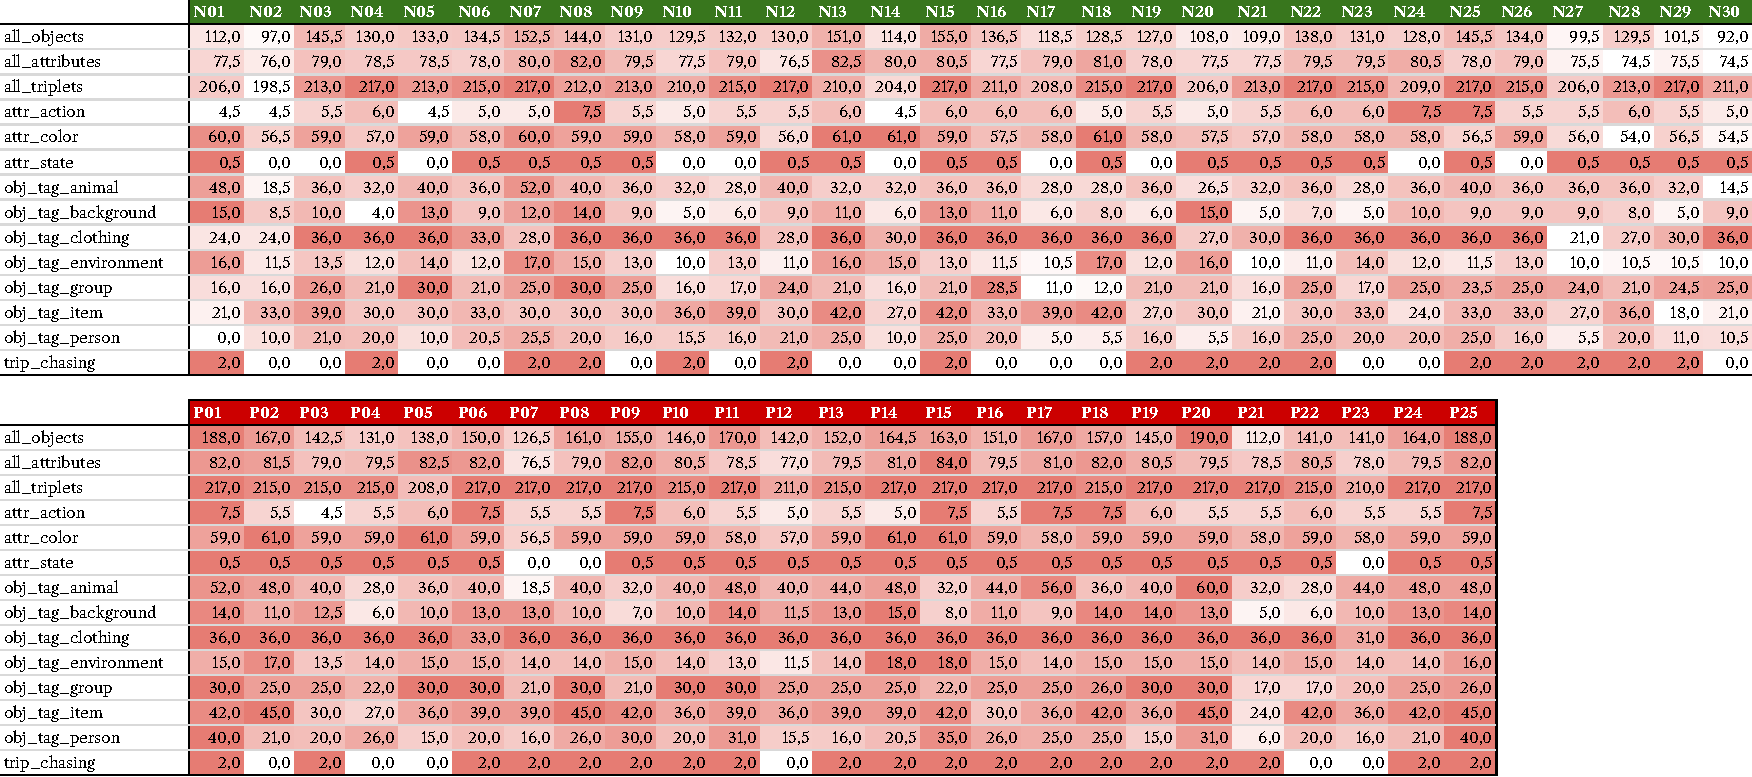
\includegraphics[width=0.86\paperheight]{./src/imgs/merged_v2.pdf}
		\caption{Vizuální znázornění rozdílných ztrát pro bez osoby bez diagnózy (sloupce \emph{N01} až \emph{N30}) a diagnostikované pacienty (sloupce \emph{P01} až \emph{P25})}\label{tab:color_table}
	\end{table}
\end{landscape}
\restoregeometry



\clearpage
\section{Závěr}
% NOTE: co bylo cílem
Cílem této práce bylo navrhnout a implementovat systém pro hodnocení míry korespondence mezi
obrázkem a jeho popisem v přirozeném řeči.
Motivací pro takovýto systém bylo jeho využití pro usnadnění diagnostických testů pro detekci kognitivních poruch.
Zvolené řešení bylo založeno na expertním přístupu, který byl pro toto použití shledán vhodným.

% NOTE: na co byl kladen důraz
Během návrhu a realizace byl kladen důraz na to, aby všechny důležité procesy a subsystémy umožňovaly
precizní kontrolu a možnost případných detailních úprav pro dosažení co nejlepších výsledků v reálném nasazení.
Dále bylo během návrhu dbáno na modularitu a obecnost, aby bylo možné jednotlivé procesy nahradit
za případné vhodnější alternativy pro konkrétní aplikace v různých oblastech.

% NOTE: jak dopadla architektura
Výsledná architektura celého systému se skládá z referenčního popisu obrázku, subsystému pro zpracování přirozené
řeči a extrakce sémantické informace, která je v ní obsažena, a hodnotícího algoritmu,
který porovná referenční popis se získanou sémantikou a na základě ztrátové tabulky vygeneruje
vektor hodnot, které reprezentují míru sémantické shody mezi vzorovým a testovaným popisem.
Tento výstupní vektor je pak možné použít jako výchozí bod pro další zpracování, například jako vektor příznaků pro klasifikační metody.

% NOTE: popis procesu, výhody a nevýhody jednotlivých částí
% Celkový návrh systému je založený na expertním přístupu k řešení dané problematiky.
Od lidského experta v daném oboru je vyžadováno, aby vybral obrázek a sestavil jeho referenční popis, který udává,
jak by měl vypadat ideální popis vybraného obrázku.
Dále je nutné vytvořit gramatiku pro sémantické zpracování řeči a nakonec je na expertovi, aby vytvořil podle referenčního popisu
ztrátovou tabulku, pomocí které specifikuje závažnost různých druhů chyb v popisu.

% NOTE: jaké jsou omezení a nevýhody
Tento expertní přístup s sebou přináší omezení ve smyslu vysokých počátečních nákladů a náročné přípravy,
jelikož tvorba referenčního popisu, gramatik a ztrátové tabulky může představovat časově náročný úkol.
Na druhou stranu ale zvolený přístup umožňuje velmi detailní a precizní kontrolu nad jednotlivými procesy a fázemi, právě
díky tomu, že vstupní vzorová data mohou být pečlivě sestavena a nejsou generována automaticky pomocí statistických metod či neuronových sítí,
jejichž výsledky nemusí být dostačující pro takto specializovanou problematiku.

% NOTE: spgf - vedlejší produkt
V rámci implementace navržených systémů byl také navržen nový formát pro sémantické gramatiky, včetně implementace jeho parseru.
Jedná se o jednou z klíčových částí zpracování přirozené řeči a extrakci sémantické informace ve zde prezentovaném systému.
Tento nový formát, pojmenovaný \enquote{Semantic Parsing Grammar Format}, byl založen na existujícím standardu Speech Recognition Grammar Specification,
oproti kterému nabízí rozšíření funkčnosti, především ve smyslu ergonomie použití a možnostech volby z vícero parsovacích strategií.
Tento formát a k němu přidružený software je možné použít nezávisle na zbytku této práce i pro zcela jiné účely.

% NOTE: jaké byly komplikace
Během realizace se nevyskytly žádné významné technické komplikace.
Jediným výraznějším problémem byla absence expertních znalostí z oblasti medicíny zaměřující se na kognitivní poruchy,
která vedla k tomu, že vytvořený referenční popis obrázku a ztrátovou tabulku bylo možné brát pouze jako ilustrační a pro testovací účely.
To však ve výsledku nepředstavovalo výrazný problém, jelikož účelem práce bylo navrhnout systém pro výše popsaný účel,
na jehož otestování ilustrační vstupní data postačovala.


% NOTE: jak dopadly výsledky
Výsledky prezentované v kapitole~\ref{sec:vyhodnoceni} ukazují, že navržený systém je schopen extrahovat z přirozeného
textu požadované sémantické informace, za předpokladu dobře navrženého referenčního popisu a především kvalitně sestavených gramatik.
Vzhledem k již popsaným problémům s absencí expertem poskytnutých dat bylo vyhodnocení porovnávacího a hodnotícího algoritmu
obtížnější, avšak dosažené výsledky nasvědčují tomu, že skutečně méně kvalitním popisům obrázku odpovídají vyšší hodnoty
ztrát, což je v~souladu s původním předpokladem.

% NOTE: jaká jsou potenciální budoucí rozšíření
Důkladnější testování hodnotícího algoritmu je plánováno v rámci již zmíněného projektu \projekt{},
který umožní detailnější analýzu nad větším množstvím dat a spolupráci s experty z daného oboru.
Dalším potenciálním rozšířením je otestování alternativních přístupů k extrakci sémantické informace,
například s využitím dnes populárních velkých jazykových modelů (angl.~large language models, LLMs).




\clearpage
\printbibliography[title=Zdroje a použitá literatura]

\end{document}
